\chapter{Aplikacija za prepoznavanje penjačkog smjera - Alpinity}

Nakon analize postojećih rješenja i tehnološke podloge računalnog vida, ovo poglavlje opisuje softversko rješenje razvijeno u sklopu ovog rada - sustav "Alpinity". Temeljna svrha sustava je riješiti problem idenfikacije penjačkih smjerova na terenu i omogućiti penjačima izvor informacija kako bi bolje organizirali vlastite penjačke izlete. Sustav se sastoji od pozadinskog sustava te dva korisnička sučelja u obliku mobilne aplikacije za iOS platformu, koja predstavlja središnji alat za koritenje na terenu, i web aplikacije, namijenjene pregledu podataka na ostalim platformama. 

Mobilna aplikacija za iOS platformu predstavlja središnji dio sustava "Alpinity" i namijenjena je penjačima za organizaciju penjačkih izleta, ali i za korištenje na terenu. Aplikacija kombinira standardne funkcionalnosti digitalnih vodiča s mogućnosti temeljenih na proširenoj stvarnosti. Omogućuje pregled detaljnih informacija o penjalištima, sektorima i penjačkim smjerovima. Uz to, nudi i personalizirane funkcionalnosti poput vođenja dnevnika uspona i praćenja osobne statistike. 
Ključna funkcionalnost je mogućnosti korištenja kamere uređaja radi unošenja referentnih podataka o penjačkim smjerovima i vizualizacije penjačih smjerova u stvarnom vremenu pomoću tehnologija proširene stvarnosti. Web aplikacija nudi većinu funkcionalnosti mobilne aplikacije kako bi aplikacija bila dostupna svim korisnicima. Razlika između aplikacija je što u web aplikaciji nije omogućeno dodavanje referentne slike penjačkog smjera, prepoznavanje penjačkih smjerova te rad u izvanmrežnom načinu rada. 

\section{Autentifikacija korisnika}

\subsection{Početni zaslon}

\begin{figure}[H]
  \centering
  \includegraphics[width=0.35\textwidth]{images/implementacija/first.png}
  \caption{Početni zaslon mobilne aplikacije "Alpinity"}
  \label{fig:prvi_zaslon}
\end{figure}

Prvi korak u korištenju aplikacije "Alpinity" je početni zaslon koji služi kao ulazna točka u mobilnu aplikaciju (slika~\ref{fig:prvi_zaslon}). Ovaj zaslon nudi tri opcije, prijavu, registraciju i pristup izvanmrežnom načinu rada (eng. \textit{offline mode}).

\begin{figure}[H]
  \centering
  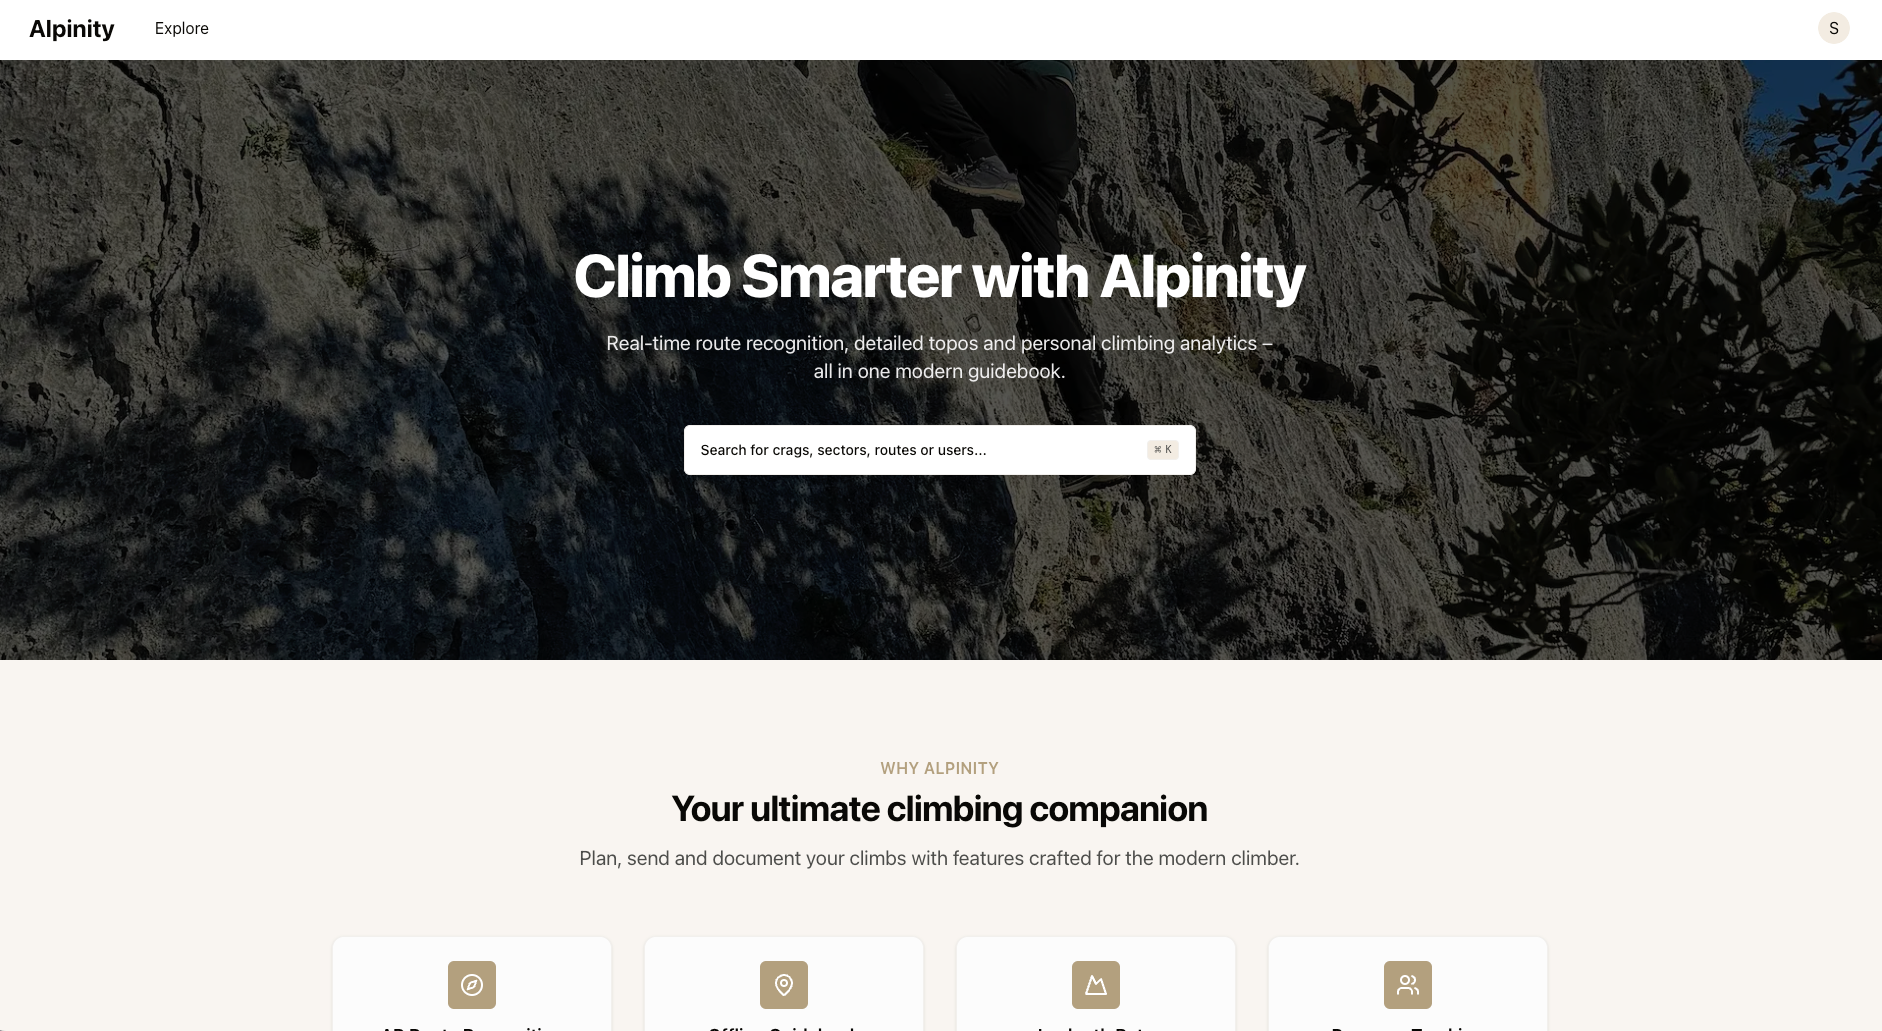
\includegraphics[width=0.9\textwidth]{images/implementacija/web/pocetni_zaslon.png}
  \caption{Početni zaslon web aplikacije "Alpinity"}
  \label{fig:prvi_zaslon_web}
\end{figure}

Na web aplikaciji, korisniku se prikazuje početni zaslon koji sadrži opis funkcionalnosti aplikacije (slika~\ref{fig:prvi_zaslon_web}). U gornjem desnom kutu nalazi se gumb za prijavu koji vodi na stranicu za prijavu iz koje se može odabrati opcija za registraciju.

\subsection{Registracija korisnika}

\begin{figure}[H]
  \centering
  \begin{subfigure}{.5\textwidth}
    \centering
    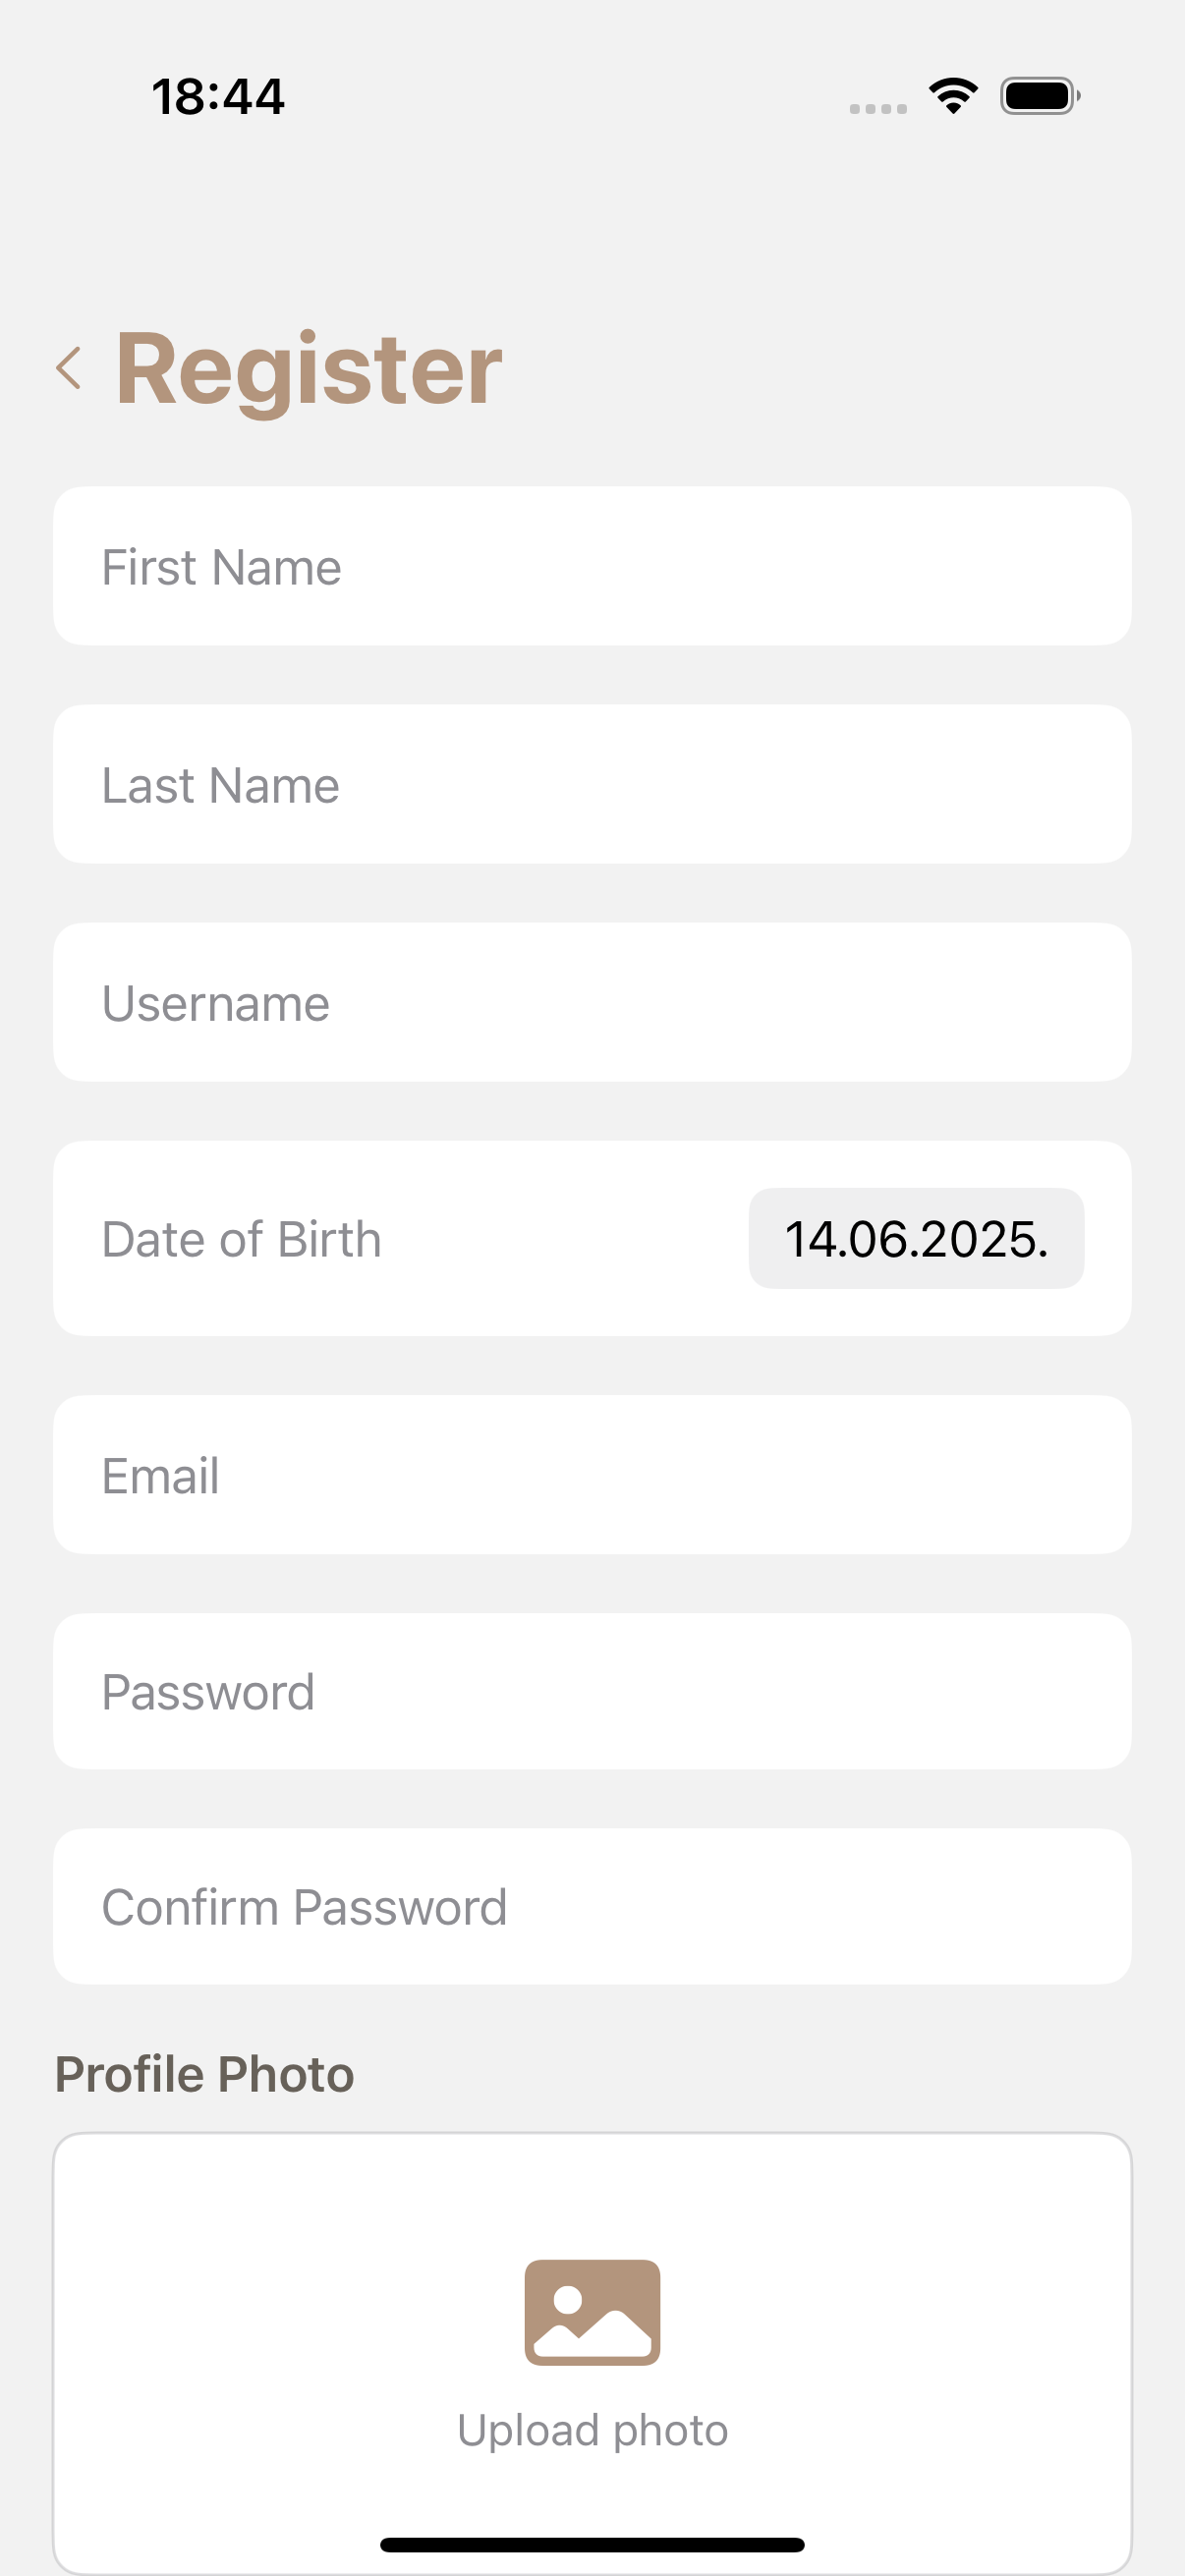
\includegraphics[width=0.7\linewidth]{images/implementacija/register.png}
    \caption{Mobilna aplikacija}
    \label{fig:registracija1}
  \end{subfigure}%
  \begin{subfigure}{.5\textwidth}
    \centering
    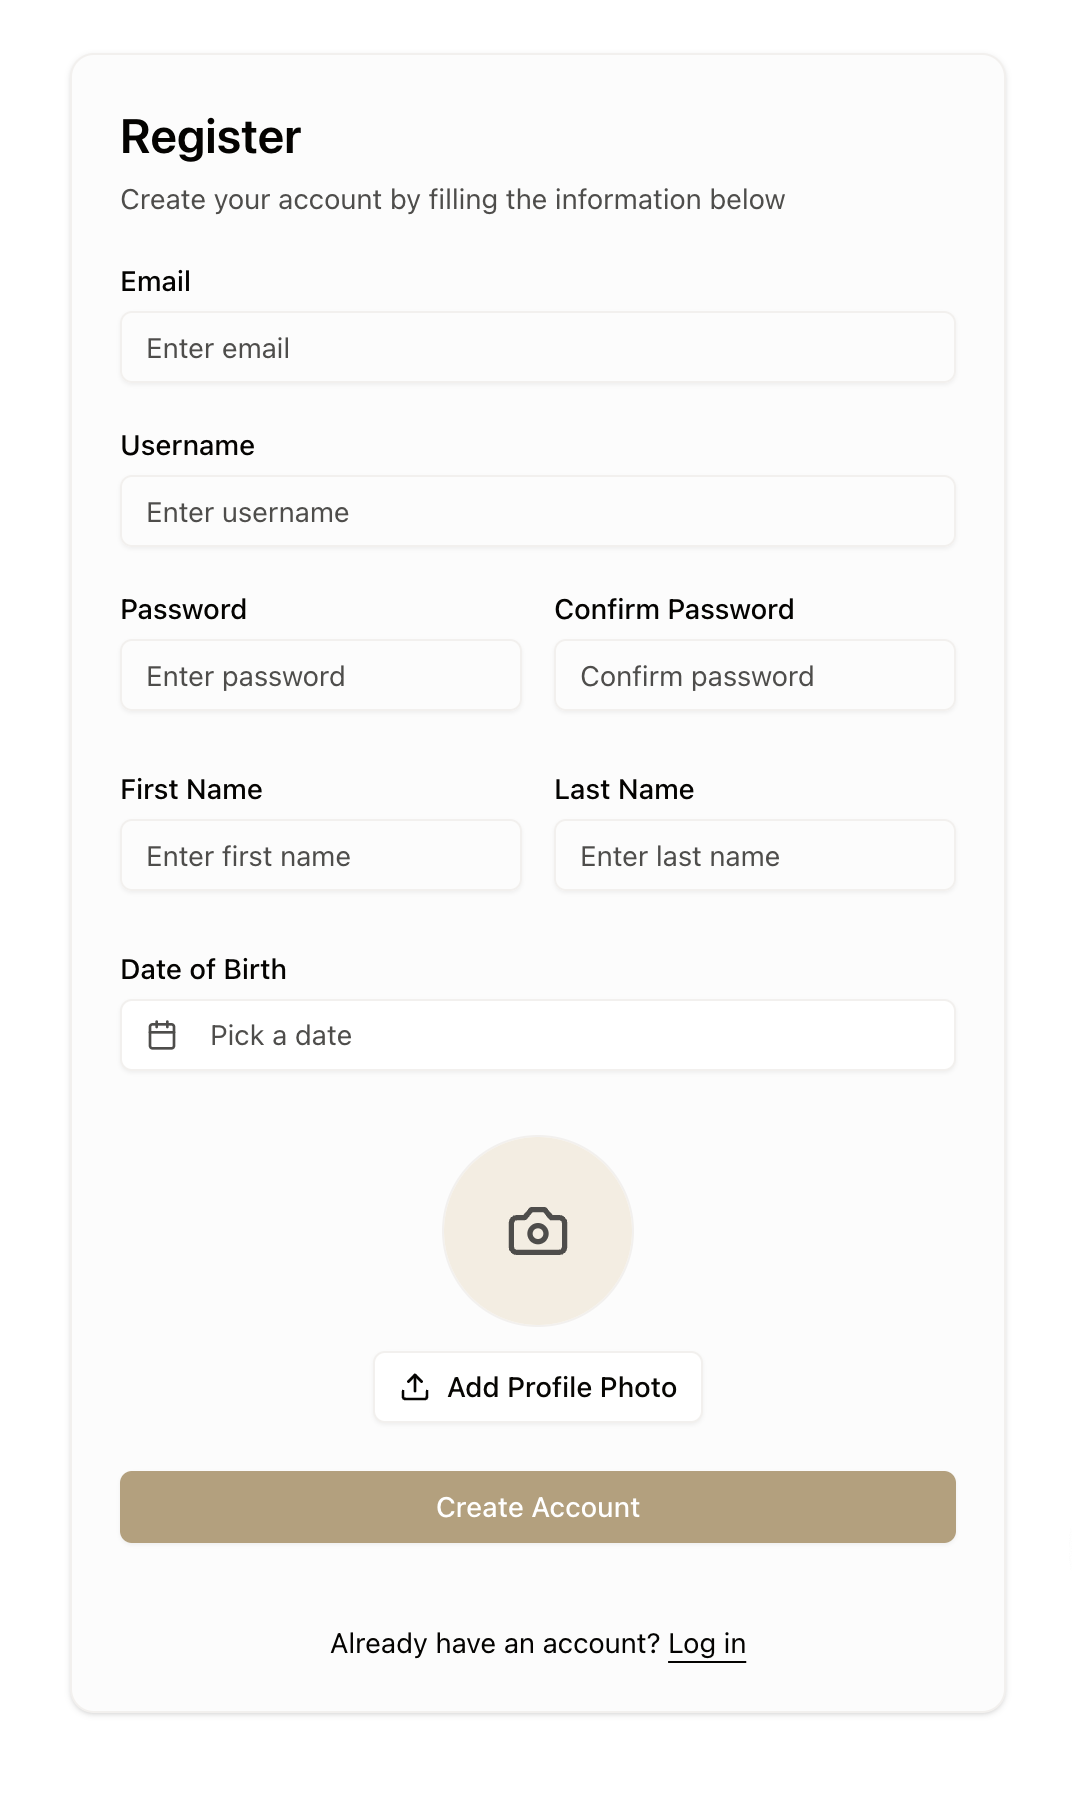
\includegraphics[width=1\linewidth]{images/implementacija/web/register.png}
    \caption{Web aplikacija}
    \label{fig:registracija2}
  \end{subfigure}
  \caption{Prikaz ekrana za registraciju korisnika u aplikaciji "Alpinity"}
  \label{fig:registracija_usporedba}
  \end{figure}


Registracija korisnika je proces kojim se stvaraju novi korisnički računi (slika~\ref{fig:registracija_usporedba}). Od korisnika se traži unos osnovnih podataka, kao što su ime, prezime, jedinstveno korisničko ime, adresa e-pošte i lozinka. Sustav također omogućuje dodavanje profilne fotografije i datuma rođenja. Proces registracije omogućuje kasnije povezivanje unesenih podataka, poput unosa u dnevnik uspona.

\subsection{Prijava korisnika}

\begin{figure}[H]
  \centering
  \begin{subfigure}{.35\textwidth}
    \centering
    
\includegraphics[width=0.9\linewidth]{images/implementacija/login.png}
    \caption{Mobilna aplikacija}
    \label{fig:prijava1}
  \end{subfigure}%
  \begin{subfigure}{.6\textwidth}
    \centering
    
\includegraphics[width=1\linewidth]{images/implementacija/web/login.png}
    \caption{Web aplikacija}
    \label{fig:prijava2}
  \end{subfigure}
  \caption{Prikaz ekrana za prijavu korisnika u aplikaciji "Alpinity"}
  \label{fig:prijava_usporedba}
  \end{figure}

Prijava korisnika omogućuje korisniku prijavu u sustav koristeći korisničko ime ili e-mail adresu te lozinku (slika~\ref{fig:prijava_usporedba}). Nakon uspješne prijave, aplikacija pohranjuje korisničku sesiju na uređaj, čime se eliminira potreba za ponovnim unosom podataka pri sljedećem pokretanju aplikacije, te korisnik je automatski preusmjeren na početni zaslon.

Nakon prijave na web aplikaciji, korisnik se vraća na početni zaslon web aplikacije gdje sada korisnik može vidjeti mogućnosti koje su dostupne samo nakon prijave poput pretraživanja te "Istraži" (eng. \textit{Explore}) stranice.


\subsection{Odjava korisnika}

Odjava korisnika je proces kojim se korisnik odjavi iz sustava. Korisnik se može odjaviti na preko vlastitog profila, gdje se nalazi gumb "Odjava" (eng. \textit{Logout}) u izborniku. Nakon odjave, korisnik se vraća na početni zaslon za prijavu i prekida se korisnička sesija.

\subsection{Navigacija do izvanmrežnog načina rada}


Posebno važna funkcionalnost, istaknuta već na početnom zaslonu mobilne aplikacije, je izvanmrežni način rada. Ova opcija omogućuje korisnicima pristup prethodno preuzetim podacima o penjalištima i penjačkim smjerovima na udaljenim lokacijama s ograničenim ili nepostojećim internetskim signalom poput penjališta u prirodi. Time se osigurava da aplikacija bude koristna i u tim uvjetima.


\section{Početni zaslon i glavna navigacija}

Nakon uspješne prijave na mobilnoj aplikaciji, korisnik pristupa početnom zaslonu koji je dizajniran kao personalizirana kontrolna ploča. (slika~\ref{fig:početni_zaslon})

\begin{figure}[H]
    \centering
    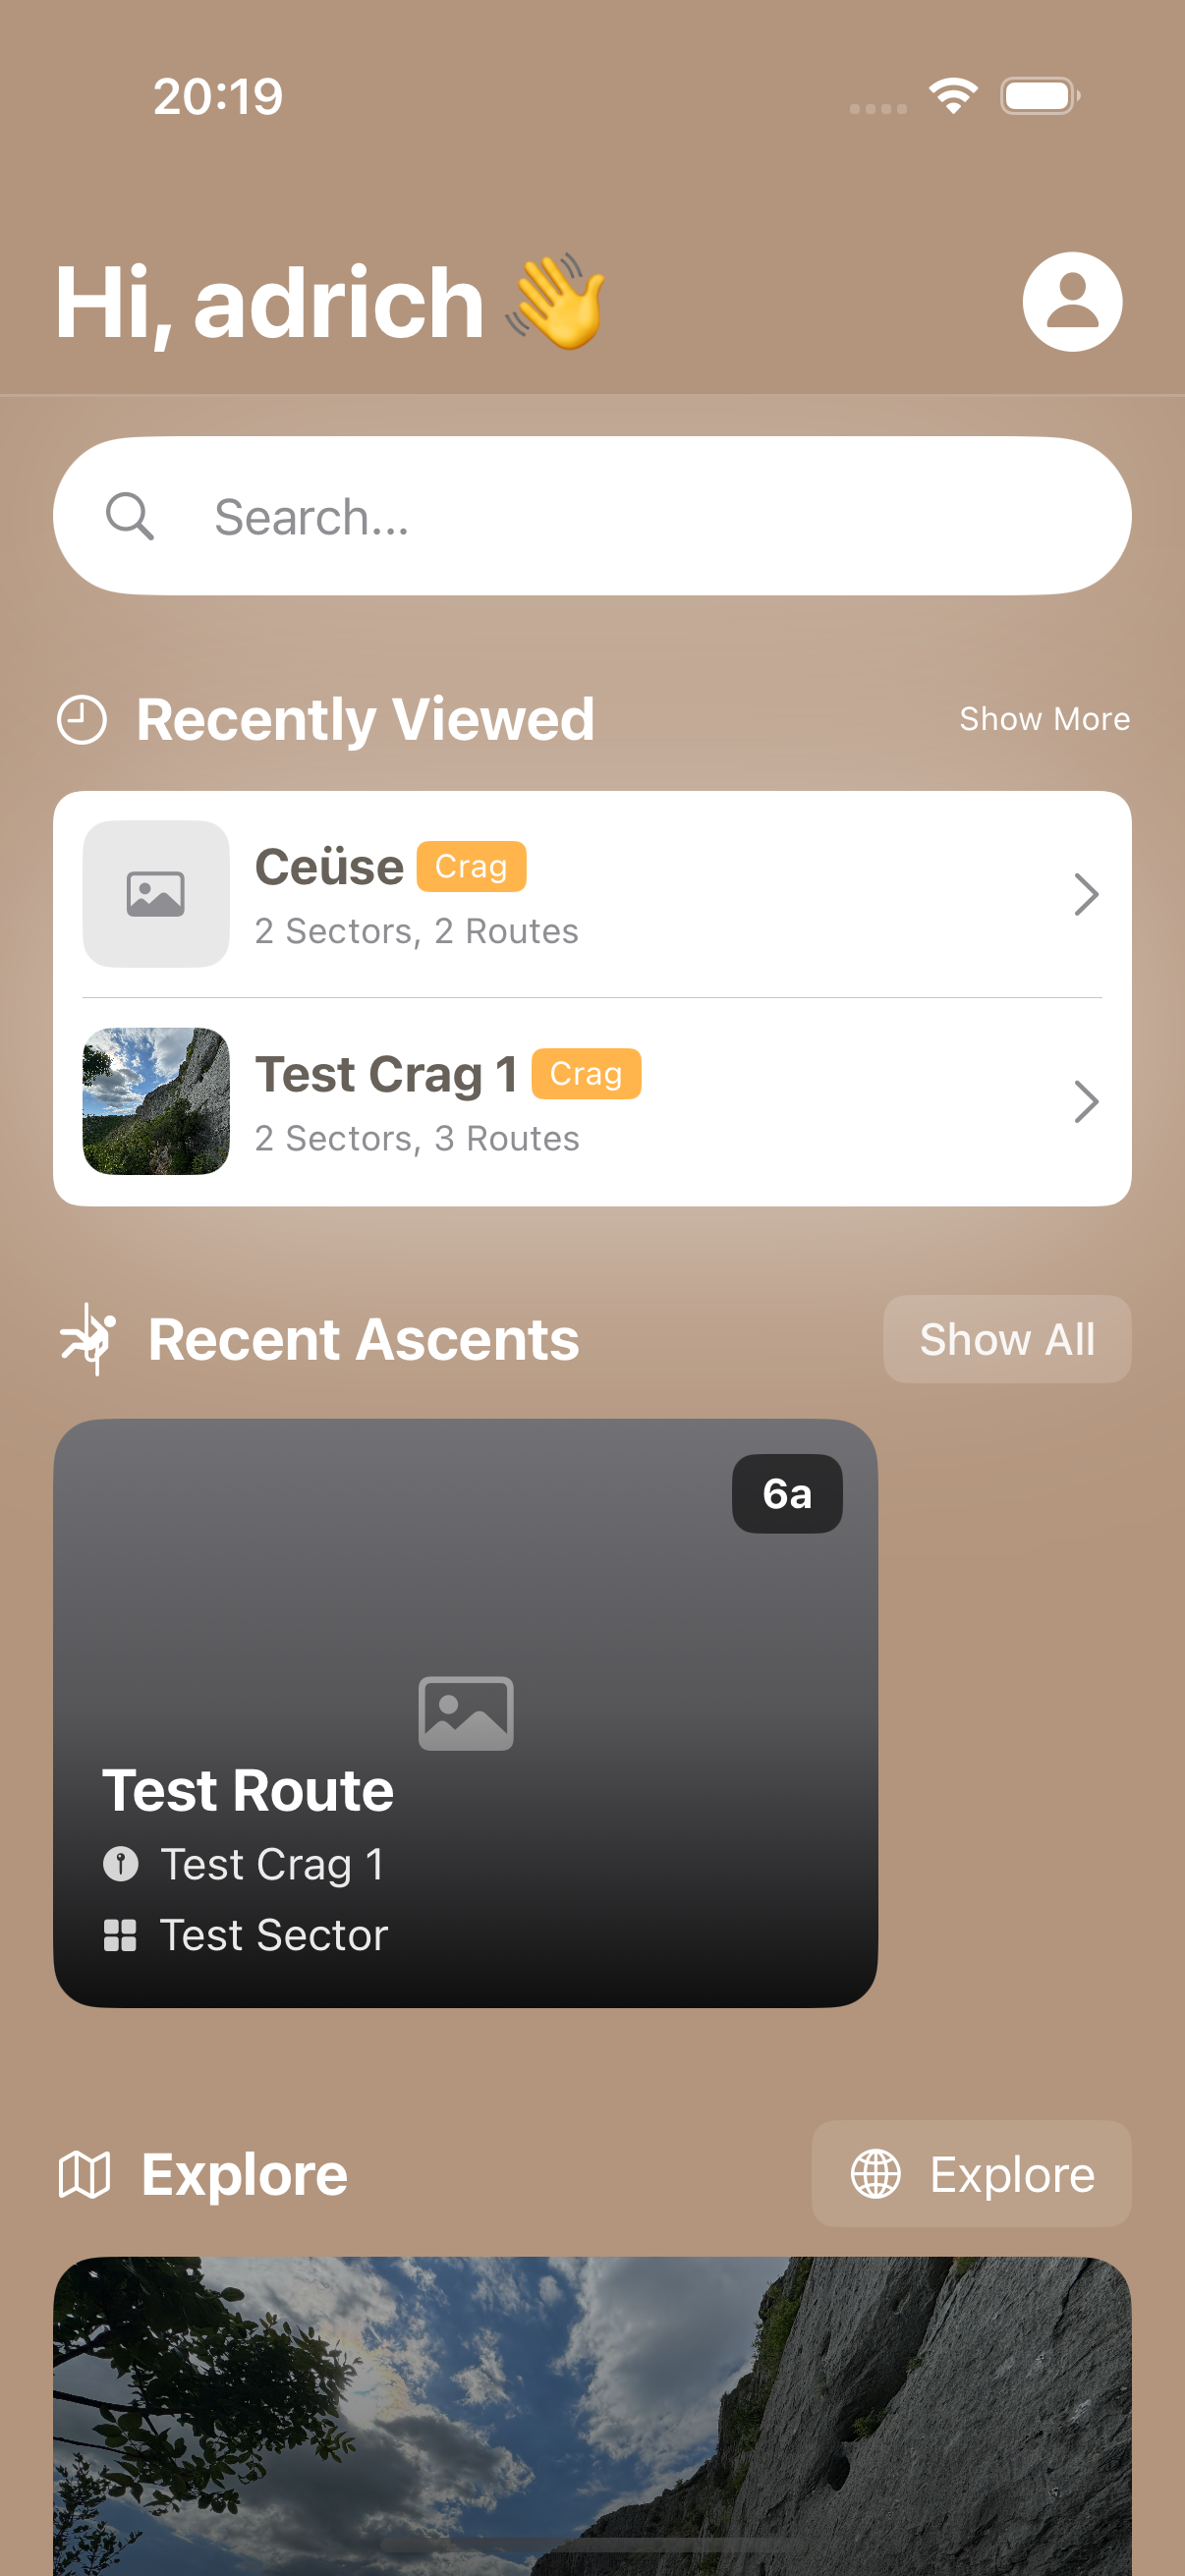
\includegraphics[width=0.35\textwidth]{images/implementacija/main_nav_1.png}
    \caption{Navigacijski zaslon aplikacije "Alpinity"}
    \label{fig:početni_zaslon}
\end{figure}

Ovaj zaslon omogućuje brzi pristup najvažnijim informacijama i funkcionalnostima. Zaslon je organiziran u nekoliko cjelina. Na vrhu zaslona nalazi se personalizirana dobrodošlica, gumb koji vodi korisnika na detalje korisničkog profila te istaknuto polje za pretraživanje koje omogućuje brzu i direktnu pretragu svih penjačkih lokacija, sektora, penjačkih smjerova i korisnika.

Sekcija "Nedavno pregledano" (eng. \textit{Recently viewed}) nudi brze poveznice na detalje penjačke lokacije, sektore, penjačke smjerove i drugih korisnika koje je korisnik nedavno pregledavao. Korisnik ima opciju "Vidi više" (eng. \textit{View more}) koja nudi korisniku prikaz više poveznica koje je posjetio.

Odmah ispod, u sekciji "Nedavni usponi" (eng. \textit{Recent ascents}) nalazi se lista najnovijih uspona korisnika zabilježenih u dnevniku uspona. Pritiskom na određeni element liste otvara se pregled detalja tog penjačkog smjera. Klikom na "Pokaži sve" (eng. \textit{Show all}) otvara se pregled vlastitog profila gdje su zapisani svi korisnikovi usponi. 

Na dnu zaslona nalazi se sekcija "Istraži" (eng. \textit{Explore}) namijenjena otkrivanju novih penjačkih lokacija pomoću prijedloga popularnih lokacija. Preporuke su određene u odnosu na prijašnje korisnikove uspone, specifično preporuke su penjačke lokacije koje se nalaze u blizini lokacija koje je korisnik nedavno posjetio. Klikom na određenu penjačku lokaciju u listi odlazi se na pregled detalja te lokacije. Pritiskom na gumb "Istraži" (eng. \textit{Explore}) otvara se pregled sa geografskom kartom sa svim penjačkim lokacijama.

Na web aplikaciji ne postoji ekvivalent za početni zaslon mobilne aplikacije, već poveznice na nedavno pregledane entitete nalaze se u sklopu pretraživanja. Nedavni usponi su dostupni u sklopu stranice korisničkog profila, a "Istraži" sekcija je pretvorena u zasebnu stranicu koja sadrži geografsku kartu sa penjačkim lokacijama i prijedlozima popularnih lokacija (slika~\ref{fig:istrazivanje_web}).

\begin{figure}[H]
    \centering
    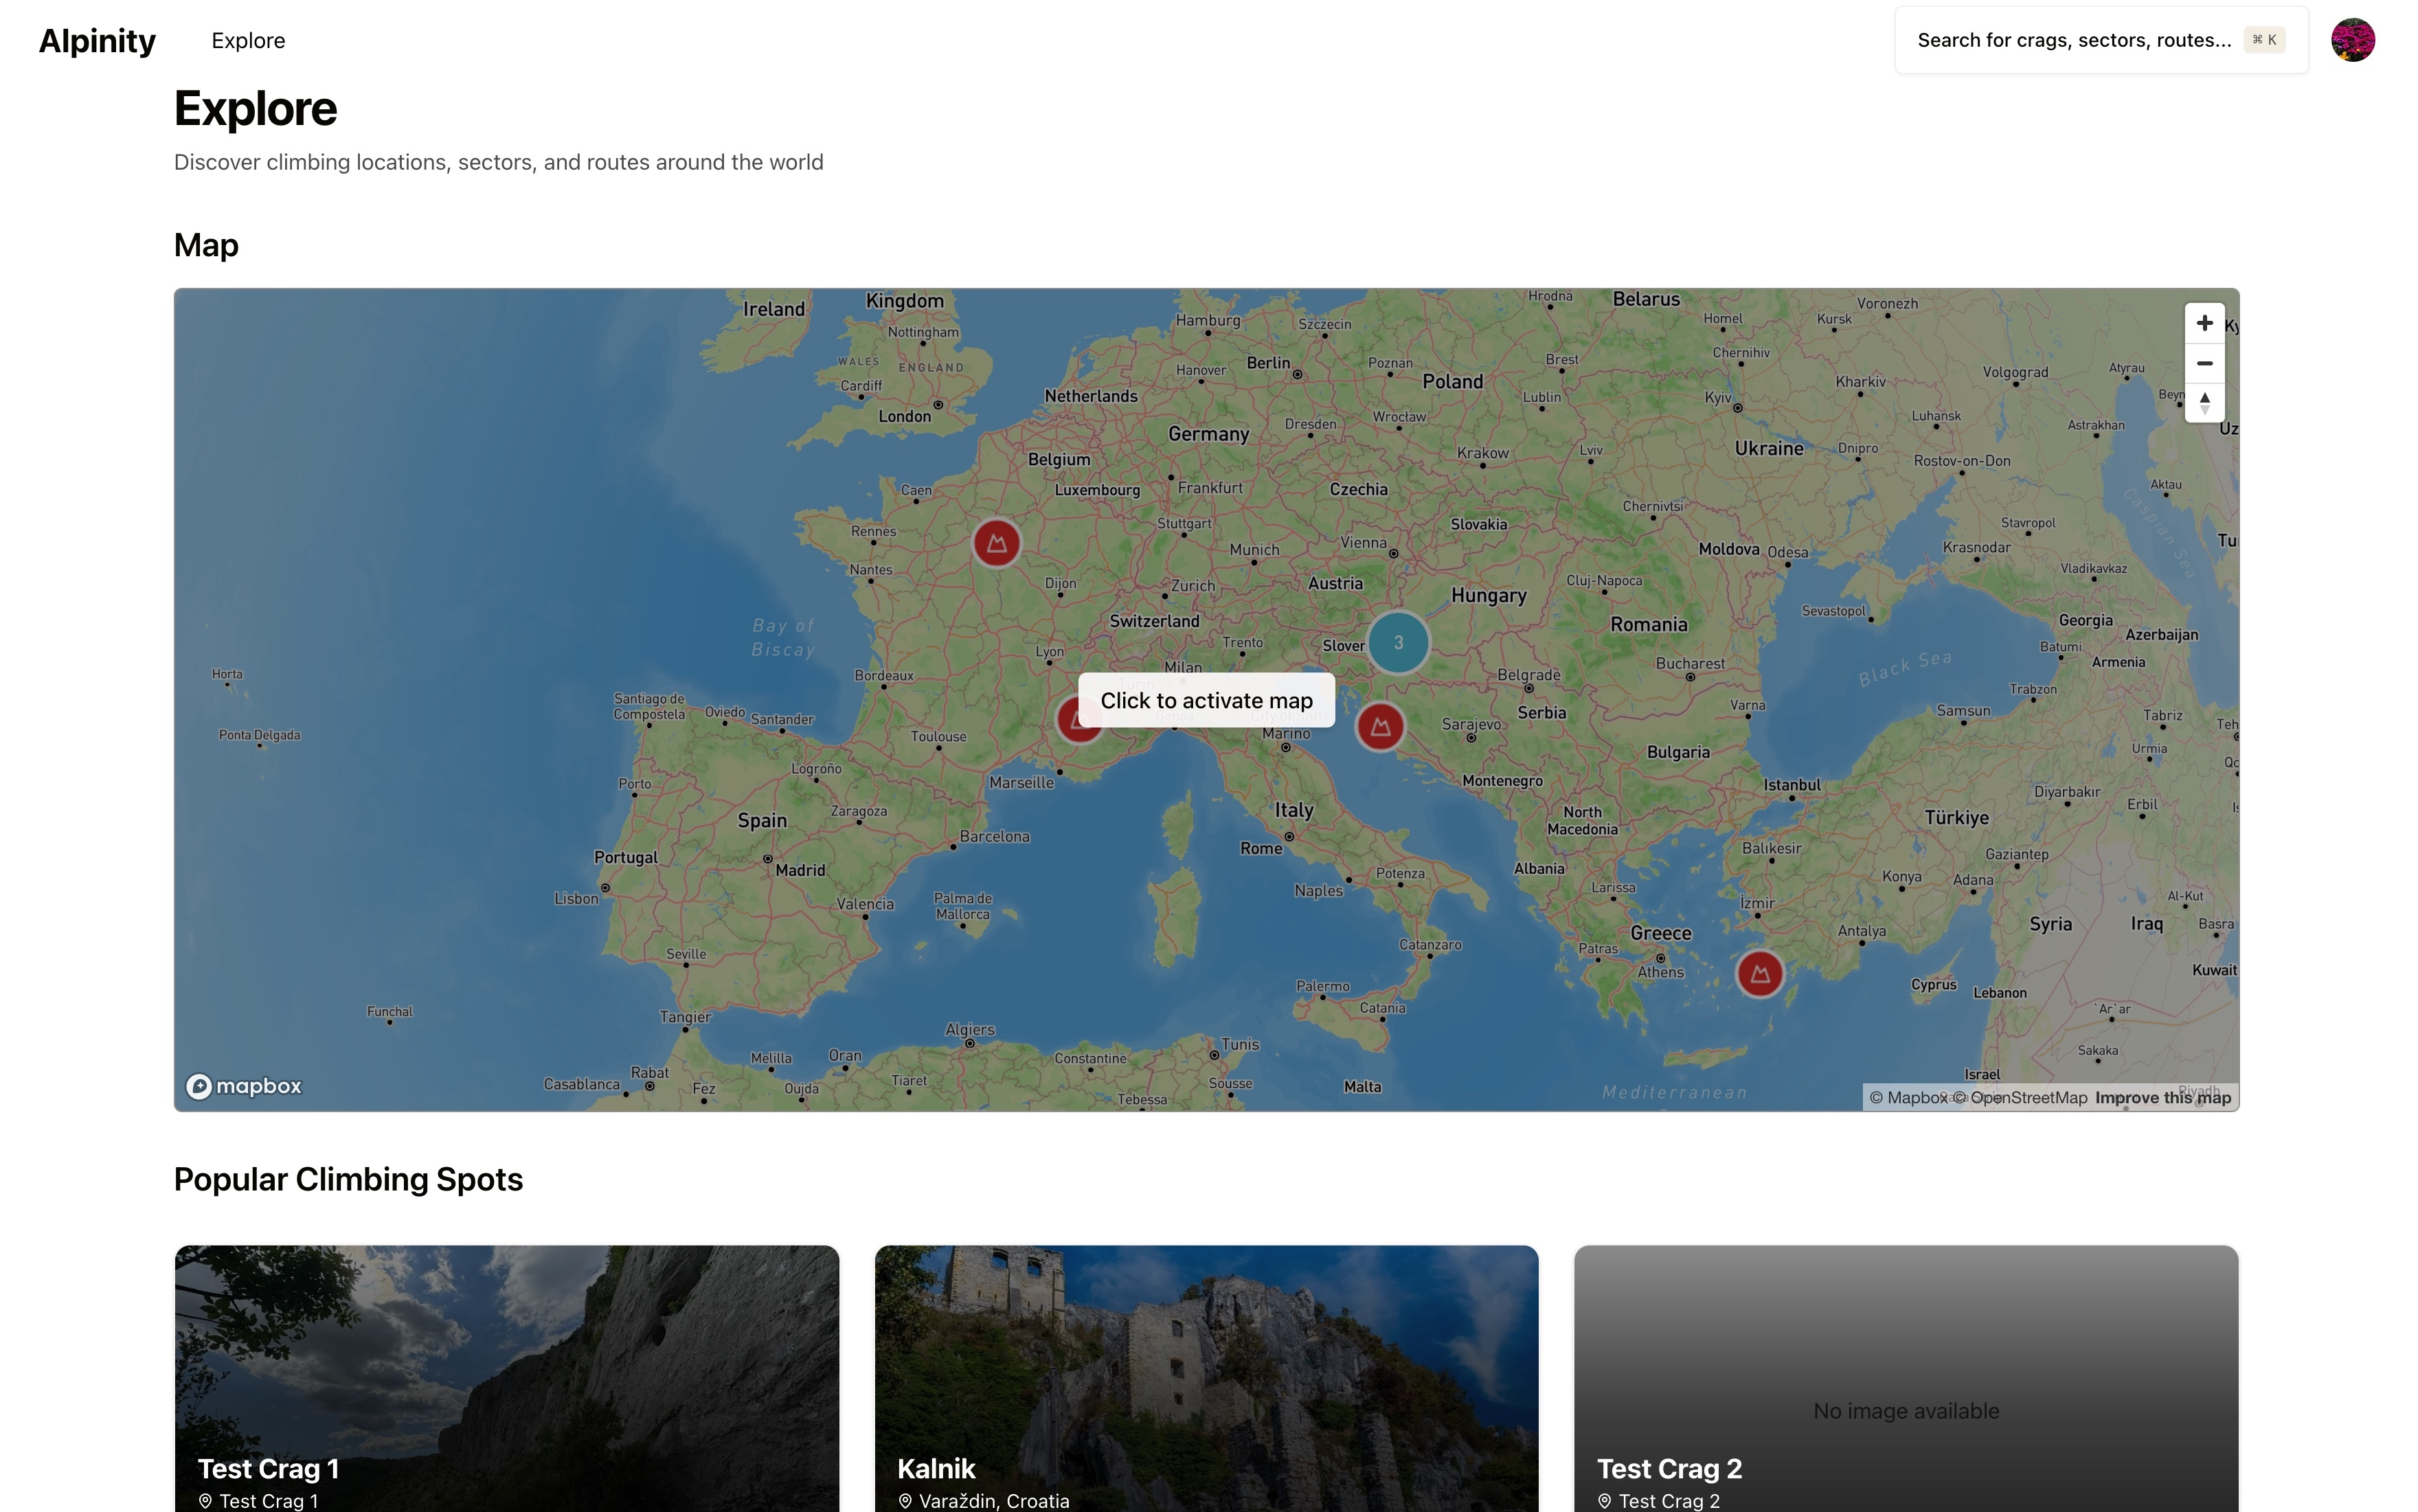
\includegraphics[width=0.9\textwidth]{images/implementacija/web/explore.jpeg}
    \caption{"Istraži" stranica web aplikacije "Alpinity"}
    \label{fig:istrazivanje_web}
\end{figure}
\section{Geografska karta penjačkih lokacija}

Kako bi se korisnicima olakšala prostorna orijentacija, aplikacije integriraju interaktivnu geografsku kartu. Ova funkcionalnost omogućuje vizualno istraživanje penjačkih lokacija na globalnoj razini kao i detaljnu navigaciju unutar pojedinog penjališta.

\begin{figure}[H]
    \centering
    \begin{subfigure}[b]{\textwidth}
        \centering
        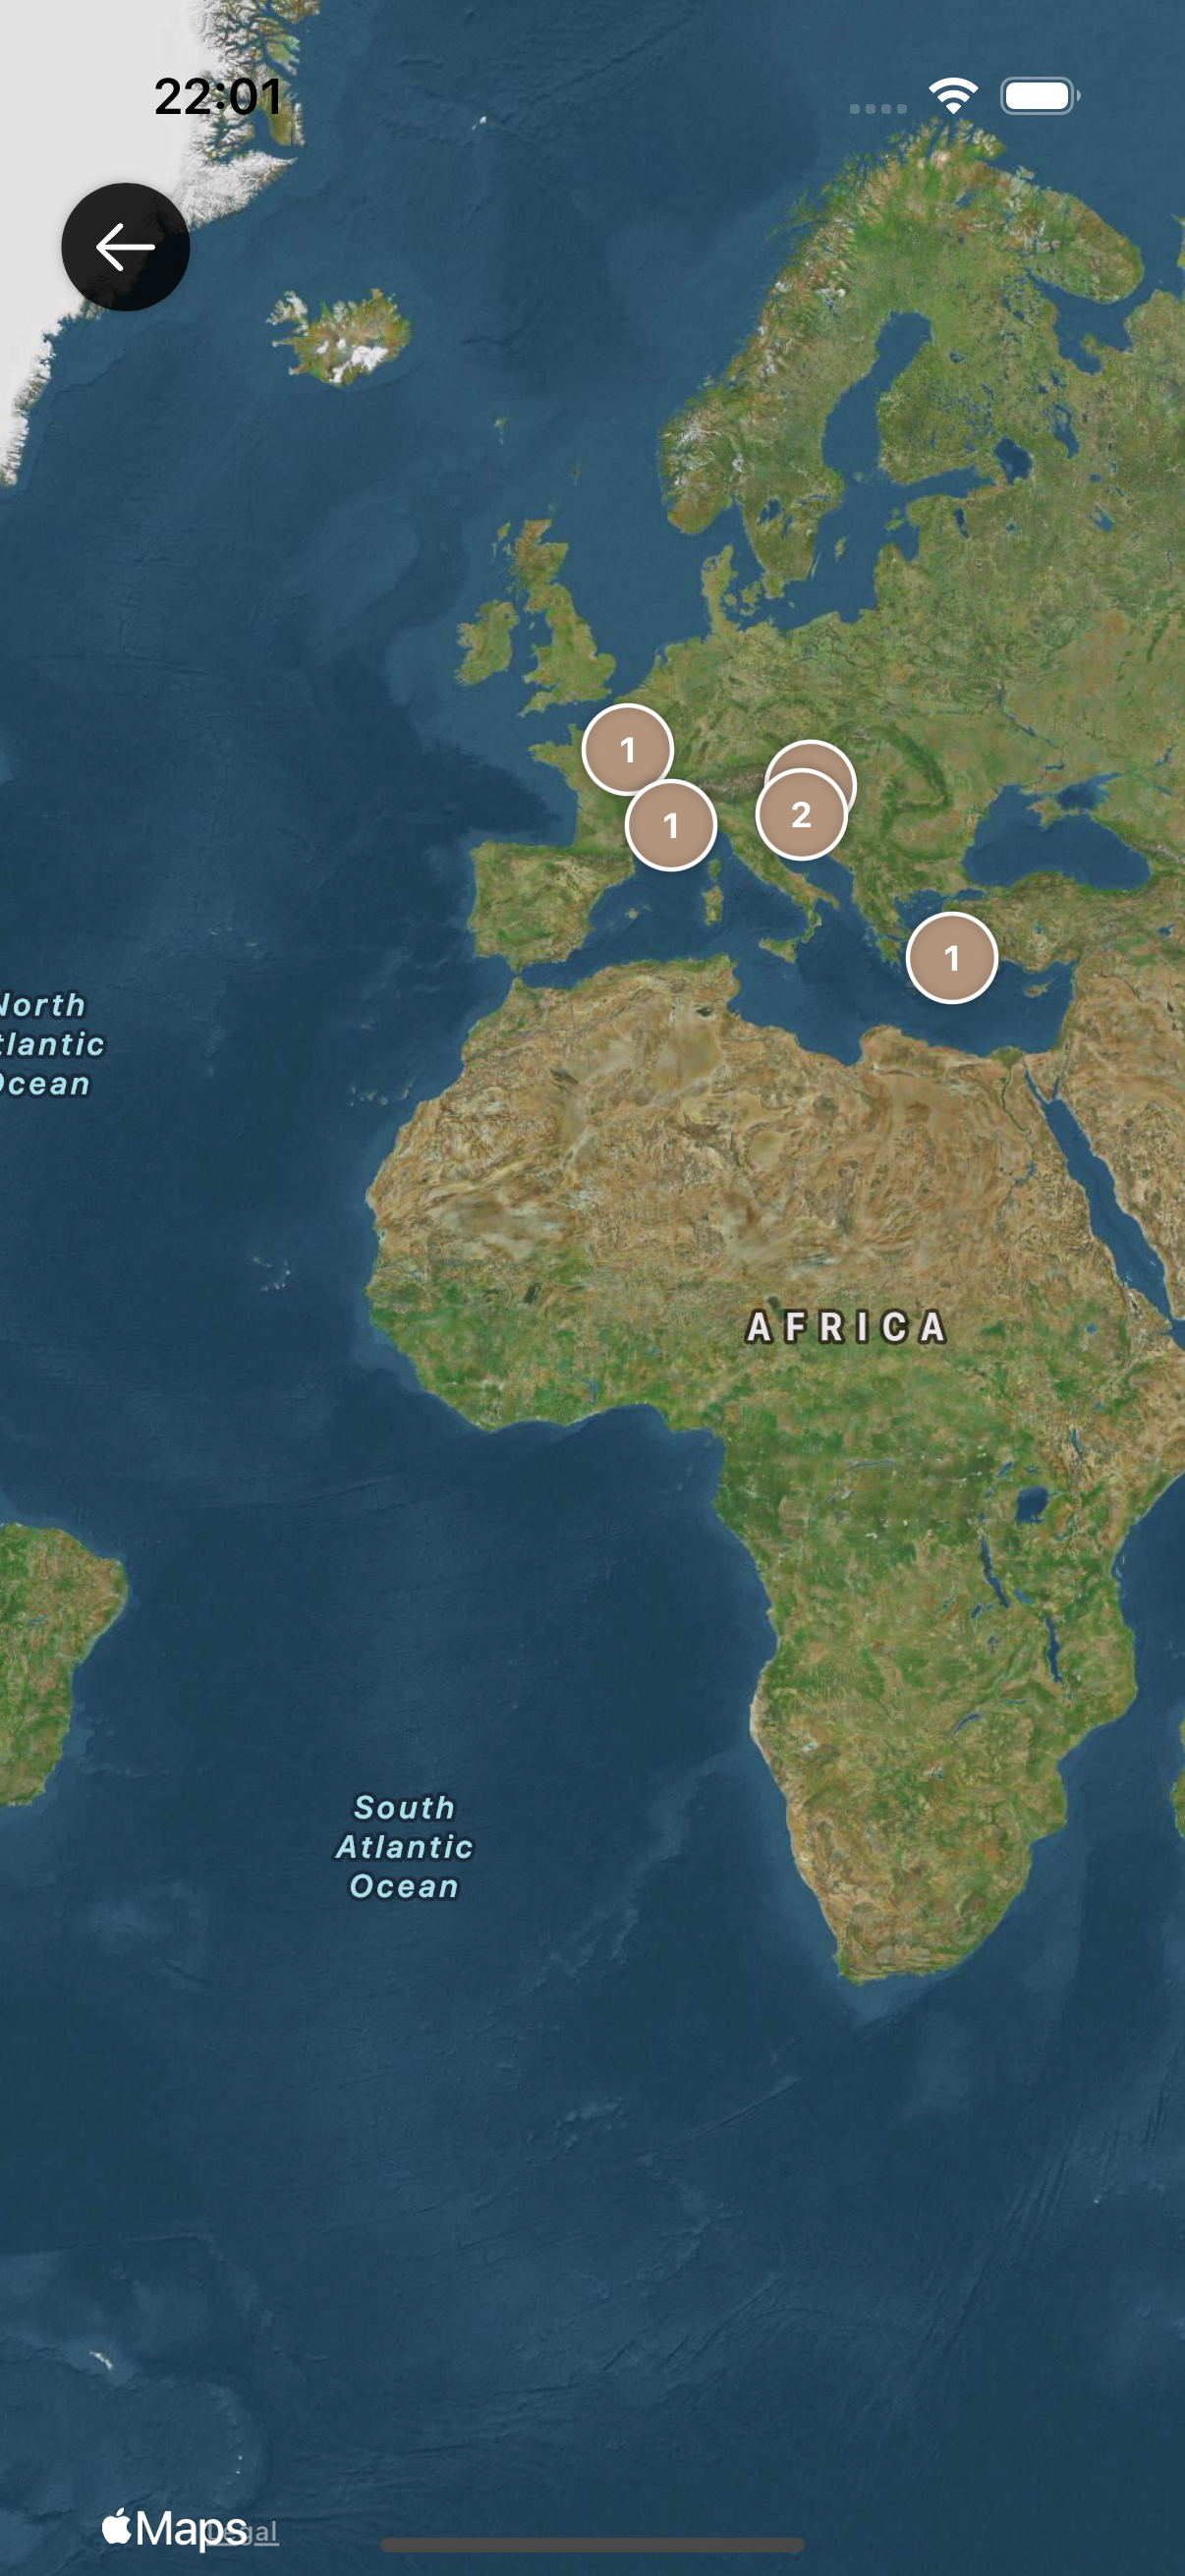
\includegraphics[width=0.3\textwidth]{images/implementacija/geo_karta.png}
        \caption{Mobilna aplikacija}
        \label{fig:geografska_karta_mob}
    \end{subfigure}
    \hfill
    \begin{subfigure}[b]{\textwidth}
        \centering
        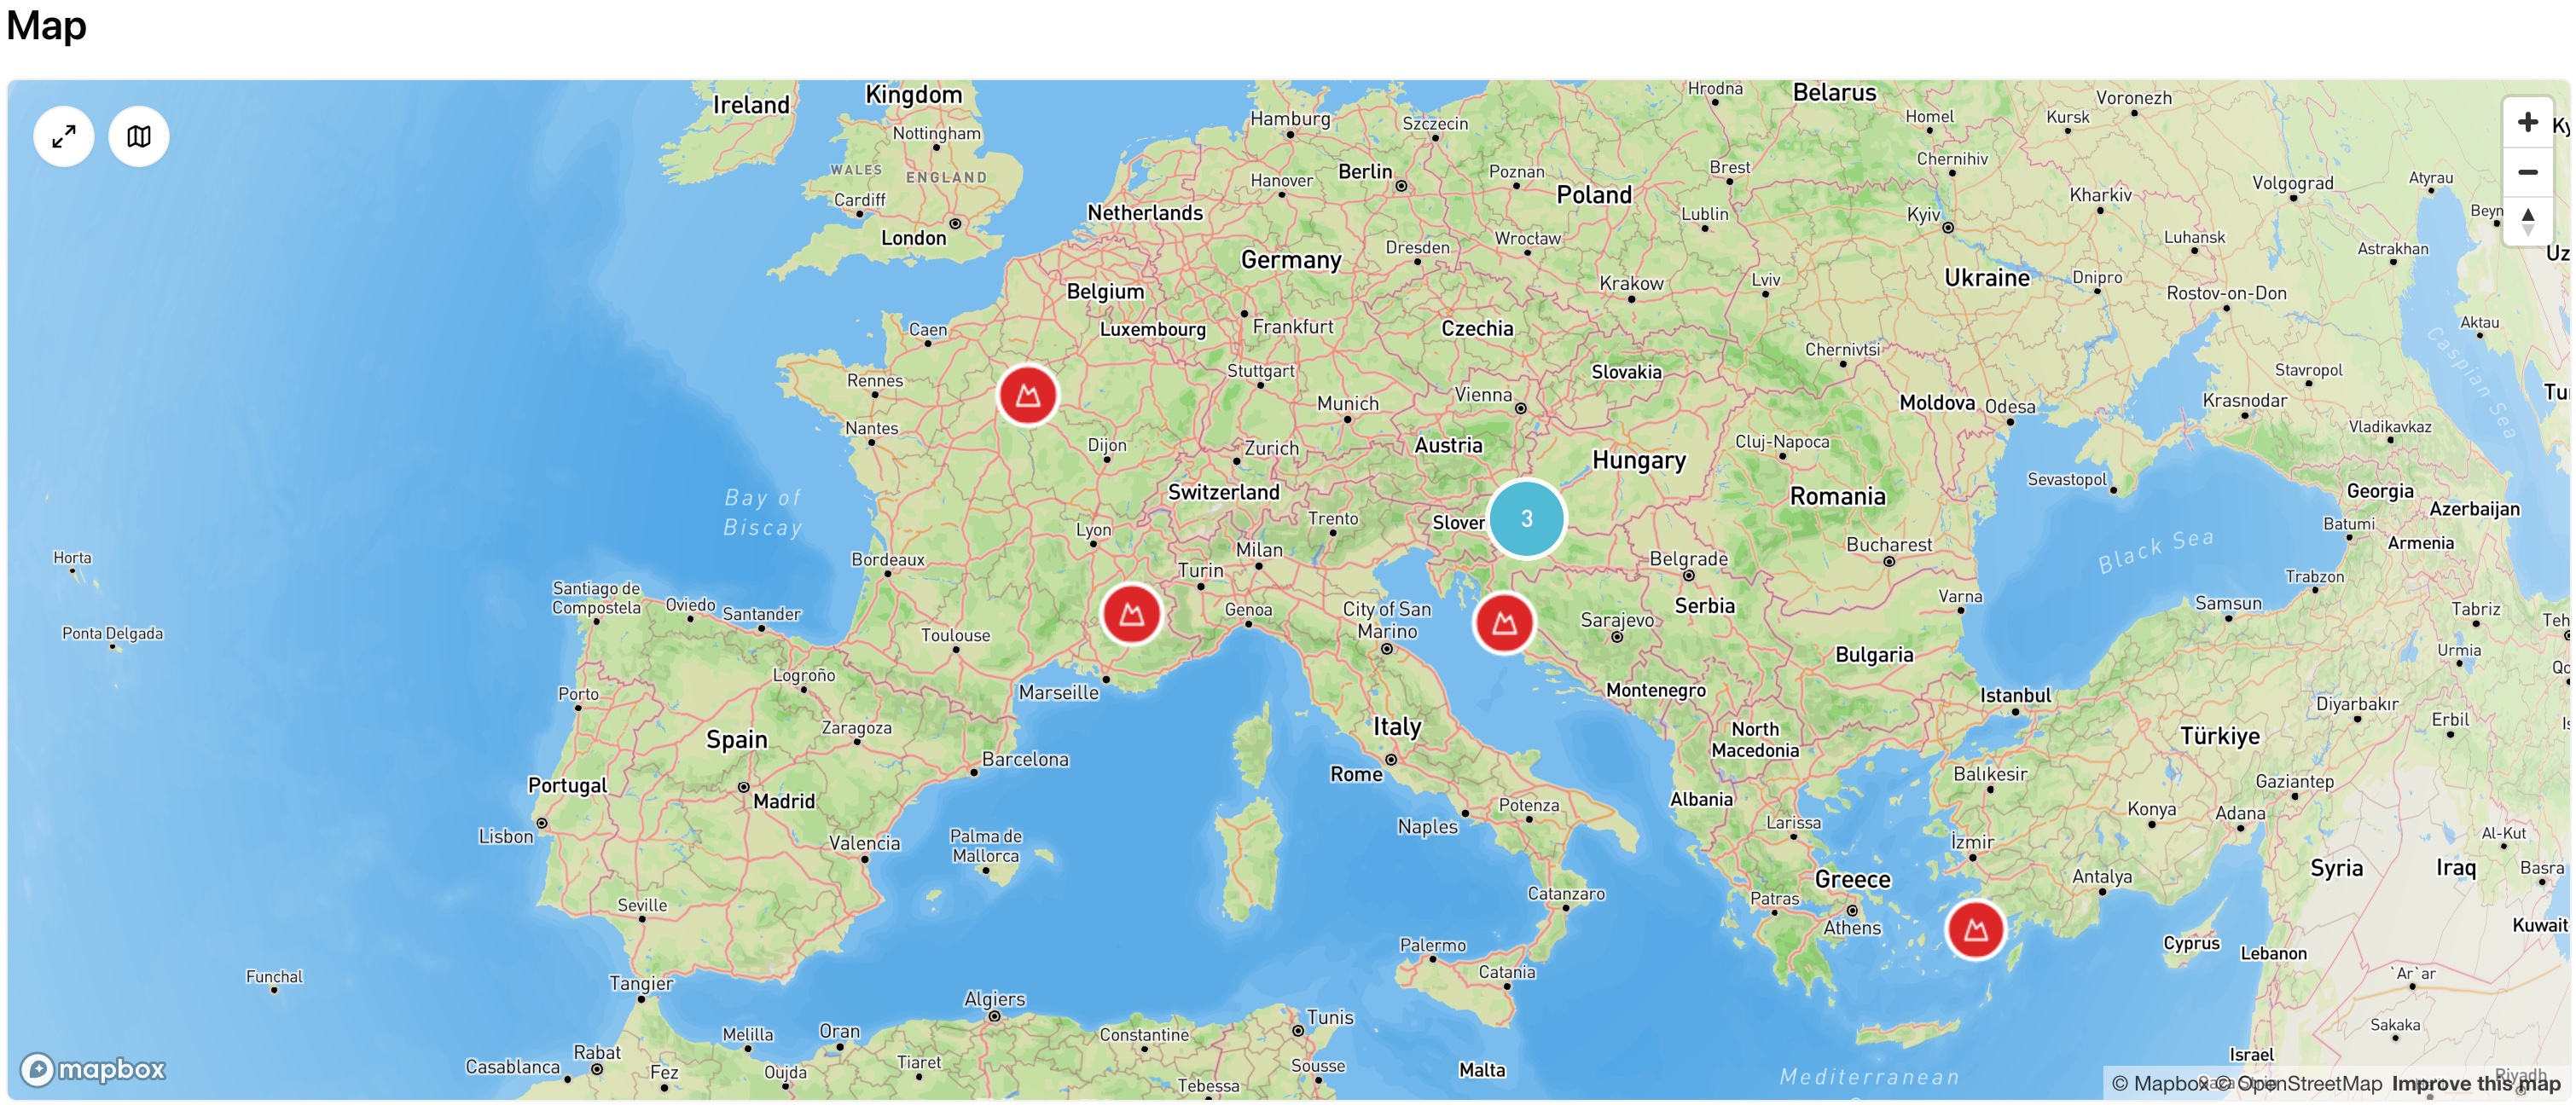
\includegraphics[width=0.9\textwidth]{images/implementacija/web/map_clusters.jpeg}
        \caption{Web aplikacija}
        \label{fig:geografska_karta_web}
    \end{subfigure}
    \caption{Geografska karta penjačkih lokacija s prikazom grupiranih oznaka}
    \label{fig:geografska_karta_sidebyside}
\end{figure}

Pristupom karti korisniku se prikazuje karta svijeta s grupiranim oznakama (eng. \textit{clusters}) koje indiciraju broj dostupnih penjališta na određenom području. Grupirane oznake omogućuju pregled prikaza na visokoj razini, ali bez pretrpanosti informacijama. Približavanjem karte, grupirane oznake se razdvajaju, otkrivajući pojedinačne lokacije penjališta.

\begin{figure}[H]
    \centering
    \begin{subfigure}[b]{\textwidth}
        \centering
        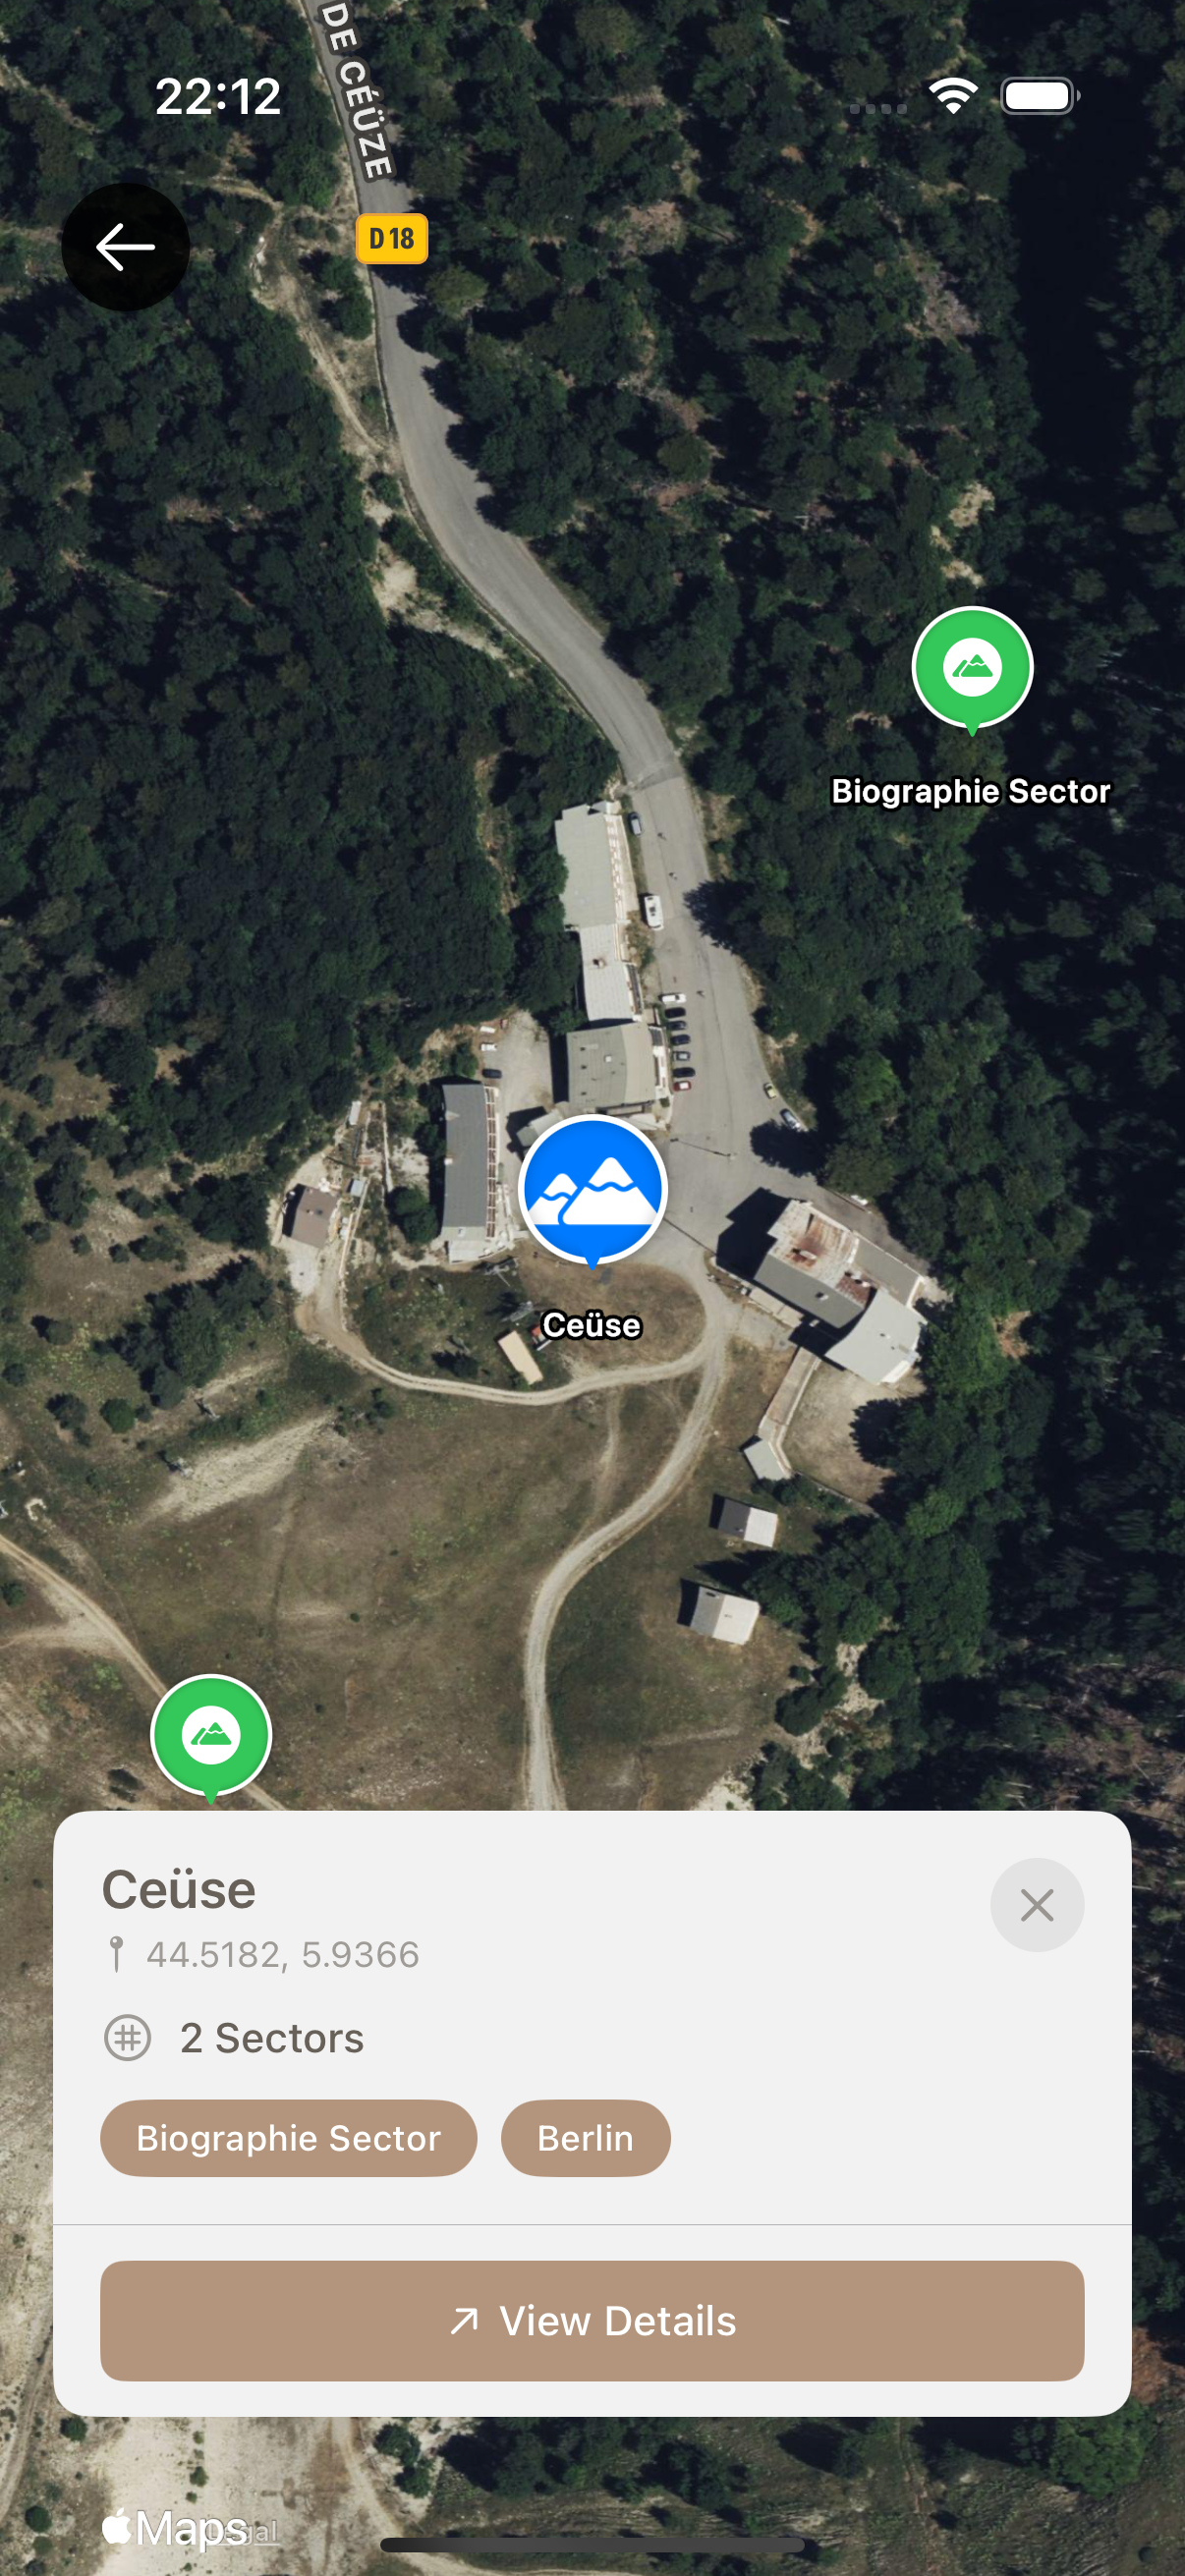
\includegraphics[width=0.3\textwidth]{images/implementacija/geo_karta_ceuse.png}
        \caption{Mobilna aplikacija}
        \label{fig:geografska_karta_ceuse_mob}
    \end{subfigure}
    \hfill
    \begin{subfigure}[b]{\textwidth}
        \centering
        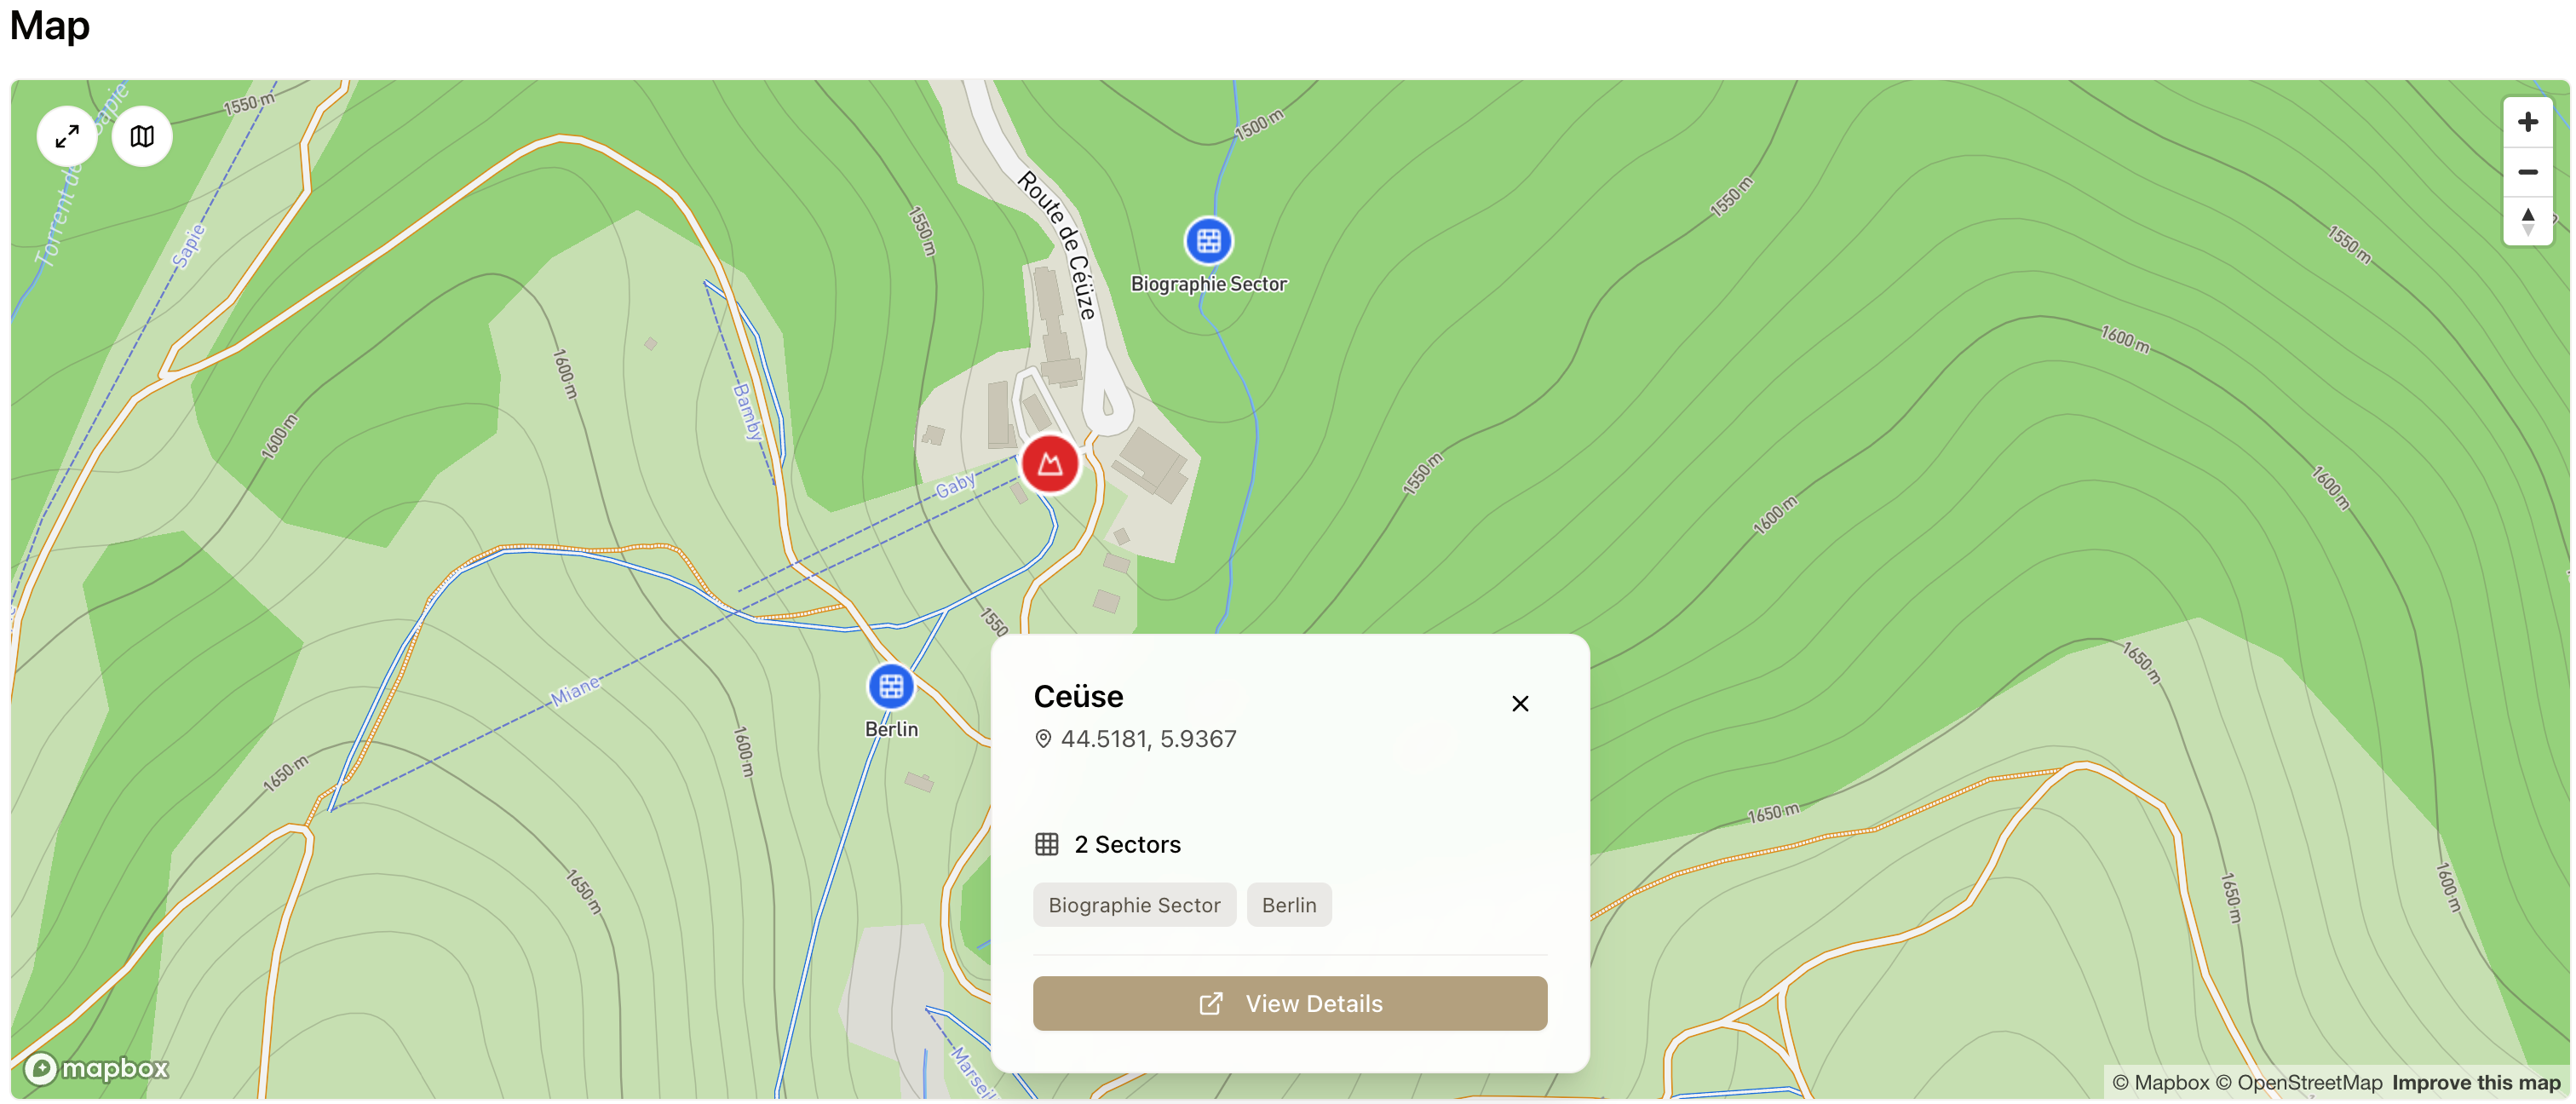
\includegraphics[width=0.9\textwidth]{images/implementacija/web/map_selected.png}
        \caption{Web aplikacija}
        \label{fig:geografska_karta_ceuse_web}
    \end{subfigure}
    \caption{Detaljan prikaz penjačke lokacije Ceuse}
    \label{fig:geografska_karta_ceuse_sidebyside}
\end{figure}

Odabirom oznake za pojedino penjalište, karta se automatski centrira i približava na tu lokaciju, prikazujući satelitski snimak područja. Na ovom detaljnom prikazu prikazana je oznaka za penjačku lokaciju, a i oznake za sve sektore. Ovakav prikaz je koristan za razumijevanje rasporeda sektora i planiranje kretanja na terenu. Na dnu prikaza nalazi se informativna kartica s osnovnim podacima o odabranoj lokaciji poput naziva, GPS koordinata i popisa dostupnih sektora. Korisniku se tada nude opcije za pregled detaljnih informacija o toj penjačkoj lokaciji ili sektorima. 

\section{Pretraživanje penjačkih lokacija, sektora, penjačkih lokacija i korisnika}

Kako bi korisnici mogli brzo pronaći informacije, aplikacija omogućuje pretraživanje penjačkih lokacija, sektora, penjačkih smjerova i korisnika. Pristupom zaslonu za pretraživanje ili na web aplikaciji klikom na traku za pretraživanje u navigacijskoj traci, korisniku se prikazuje traka za unos teksta te, inicijalno, popis nedavno pregledanih stavki, što omogućuje brz povratak na prethodno pregledane elemente (slika~\ref{fig:pretrazivanje_sidebyside}).

\begin{figure}[H]
    \centering
    \begin{subfigure}[b]{0.35\textwidth}
        \centering
        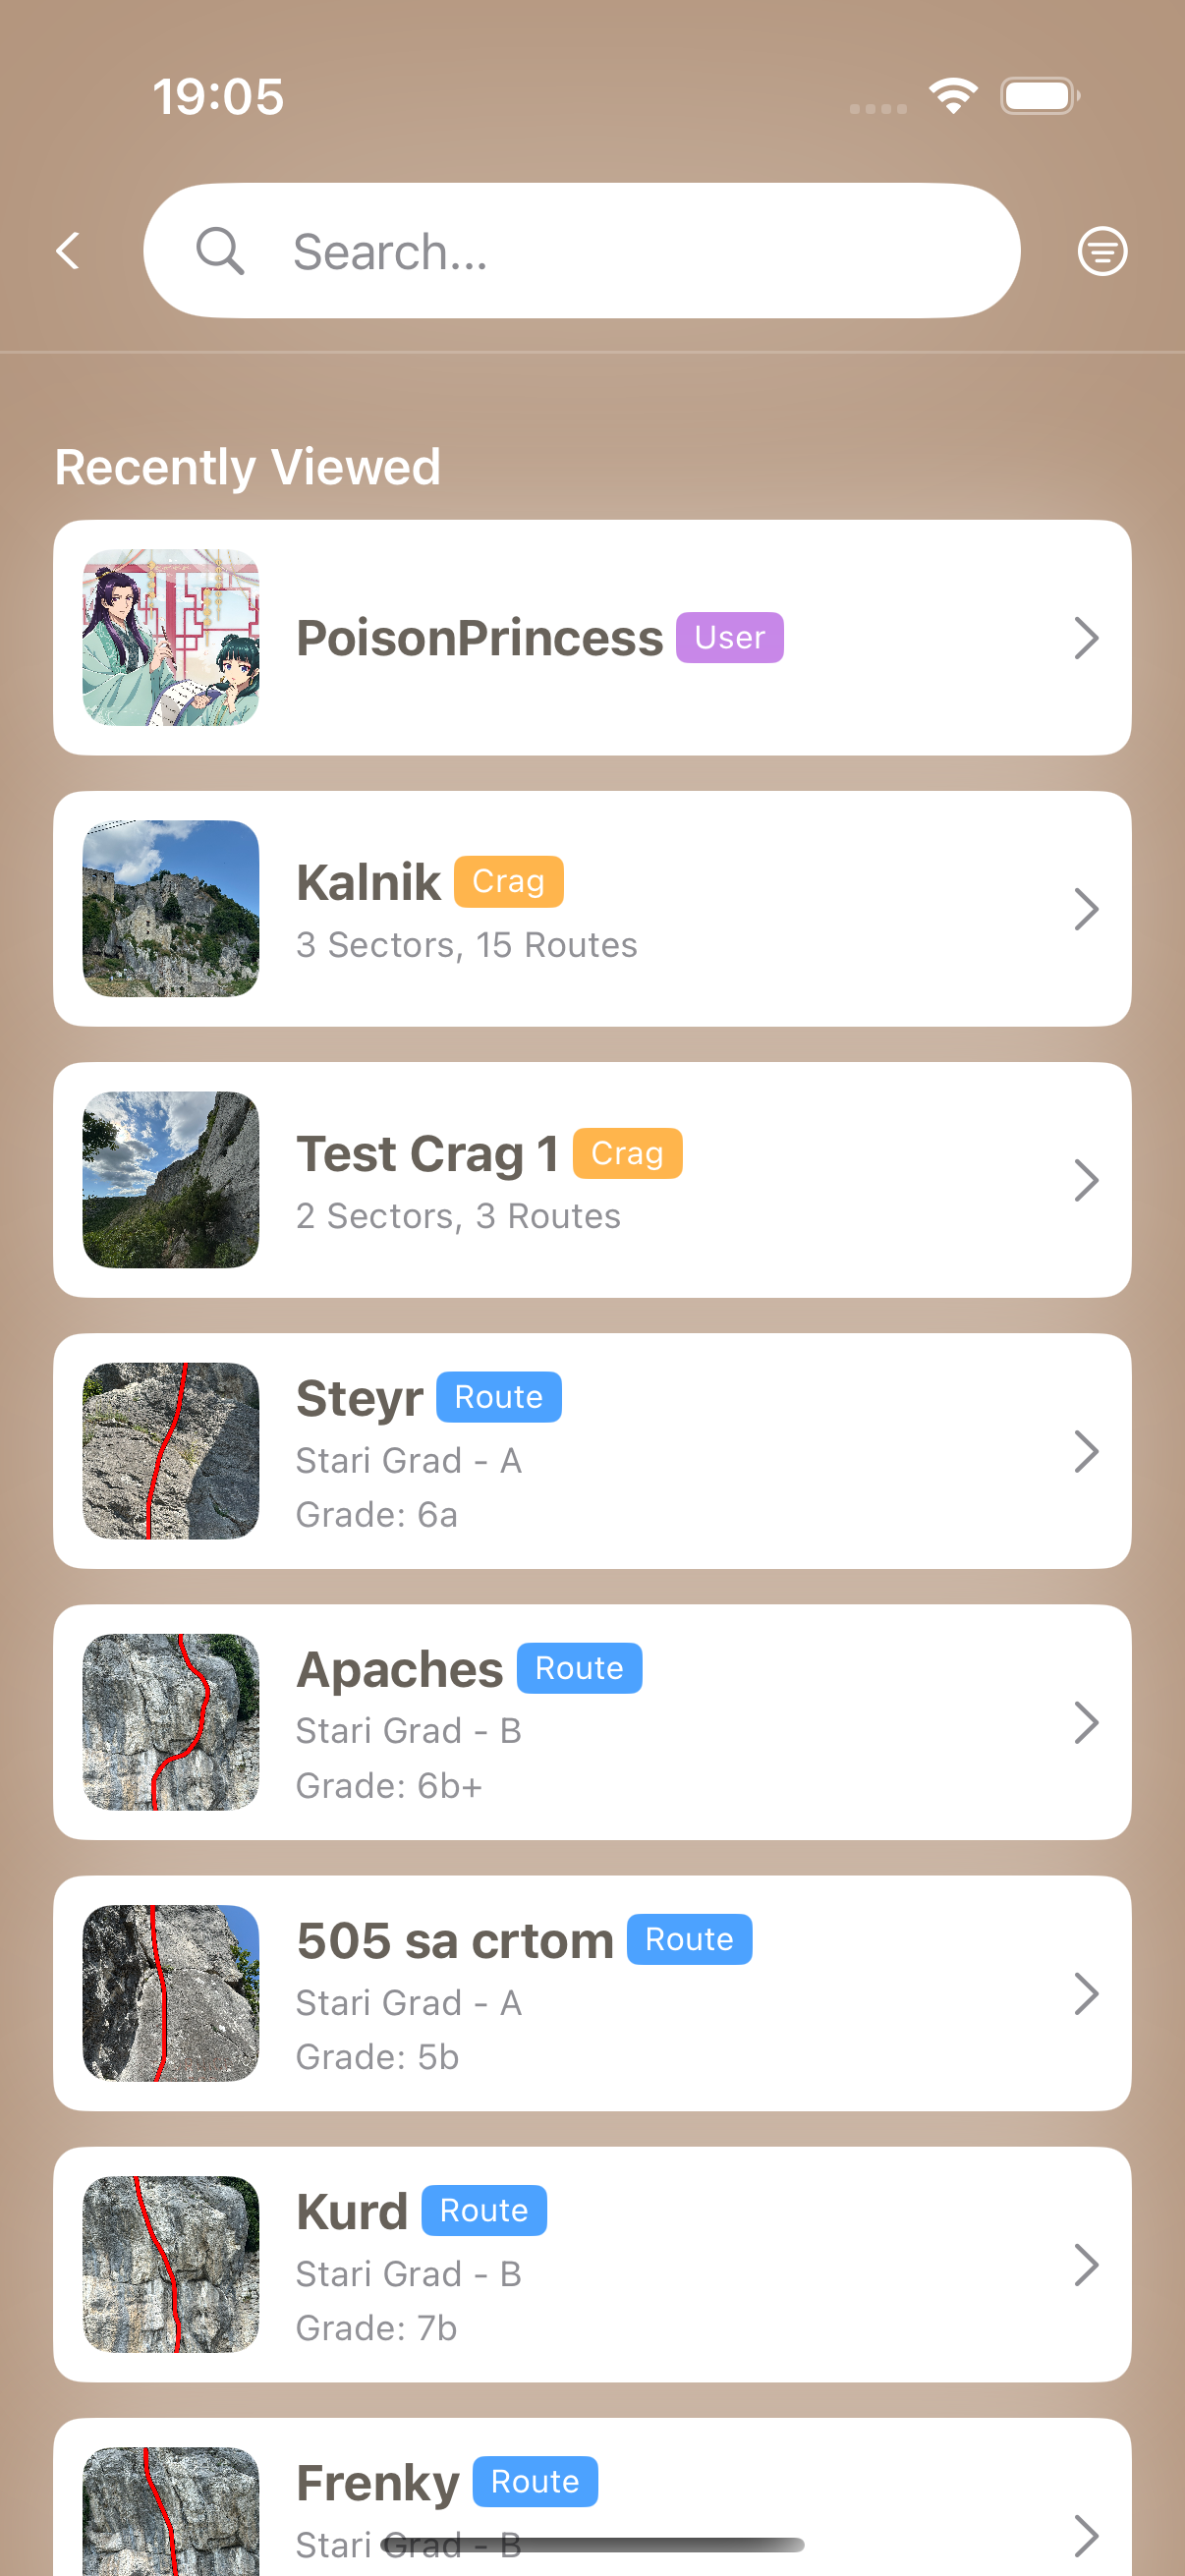
\includegraphics[width=\textwidth]{images/implementacija/search_default.png}
        \caption{Mobilna aplikacija}
        \label{fig:pretrazivanje_default}
    \end{subfigure}
    \hfill
    \begin{subfigure}[b]{0.6\textwidth}
        \centering
        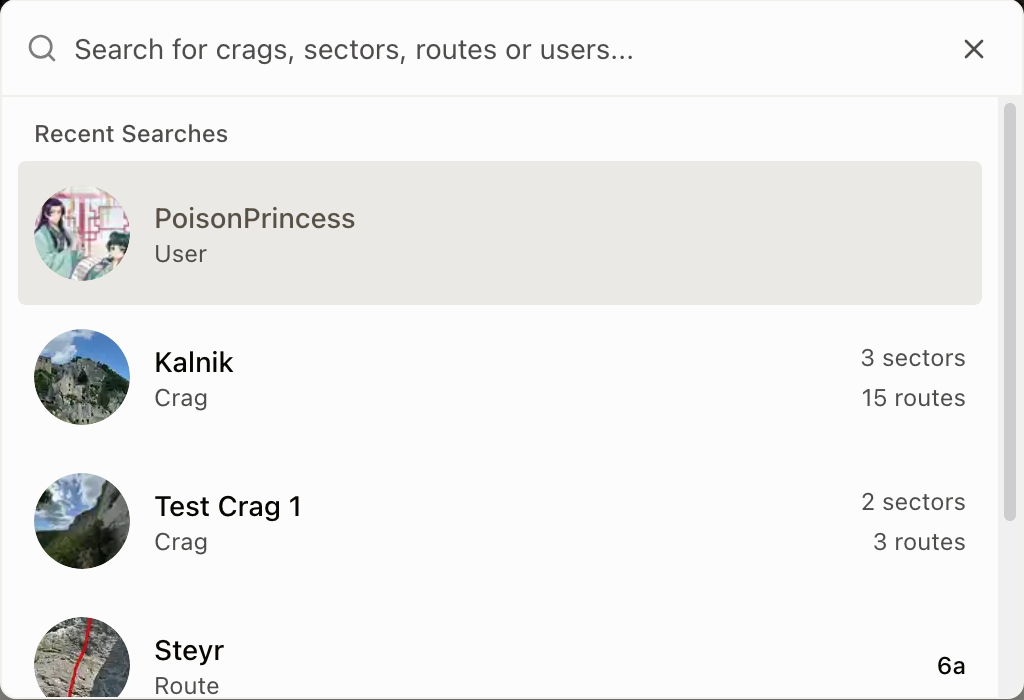
\includegraphics[width=\textwidth]{images/implementacija/web/search_default.png}
        \caption{Web aplikacija}
        \label{fig:pretrazivanje_searching}
    \end{subfigure}
    \caption{Inicijalno stanje pretraživanja - prikaz nedavno pregledanih stavki}
    \label{fig:pretrazivanje_sidebyside}
\end{figure}

Sustav pretraživanja je dinamičan i reagira na korisnikov unos. Upisivanjem pojma u traku za pretraživanje, aplikacija filtrira popis dostupnih penjačkih lokacija, sektora, penjačkih smjerova i korisnika te prikazuje relevantne rezultate iz više kategorija istovremeno (slika~\ref{fig:pretrazivanje_side_by_side}). 

\begin{figure}[H]
    \centering
    \begin{subfigure}[b]{0.35\textwidth}
        \centering
        
\includegraphics[width=\textwidth]{images/implementacija/search_searching.png}
        \caption{Mobilna aplikacija}
        \label{fig:pretrazivanje_web_1}
    \end{subfigure}
    \hfill
    \begin{subfigure}[b]{0.6\textwidth}
        \centering
        
\includegraphics[width=\textwidth]{images/implementacija/web/search_searching.png}
        \caption{Web aplikacija}
        \label{fig:pretrazivanje_web_2}
    \end{subfigure}
    \caption{Funkcionalnost pretraživanja}
    \label{fig:pretrazivanje_side_by_side}
\end{figure}

Svaki rezultat pretrage prikazan je u obliku pregleda kartica koje sadrže informacije poput naziva i tipa sadržaja, te dodatne podatke ovisno o tipu sadržaja. Penjačke lokacije sadrže broj sektora i penjačkih smjerova, sektori broj penjačkih smjerova, a korisnici broj penjačkih smjerova koje su popeli. Odabirom bilo kojeg rezultata, korisnik se preusmjerava na odgovarajući detaljni prikaz. 


\section{Detalji penjališta}

\begin{figure}[H]
    \centering
    \begin{subfigure}[b]{\textwidth}
        \centering
        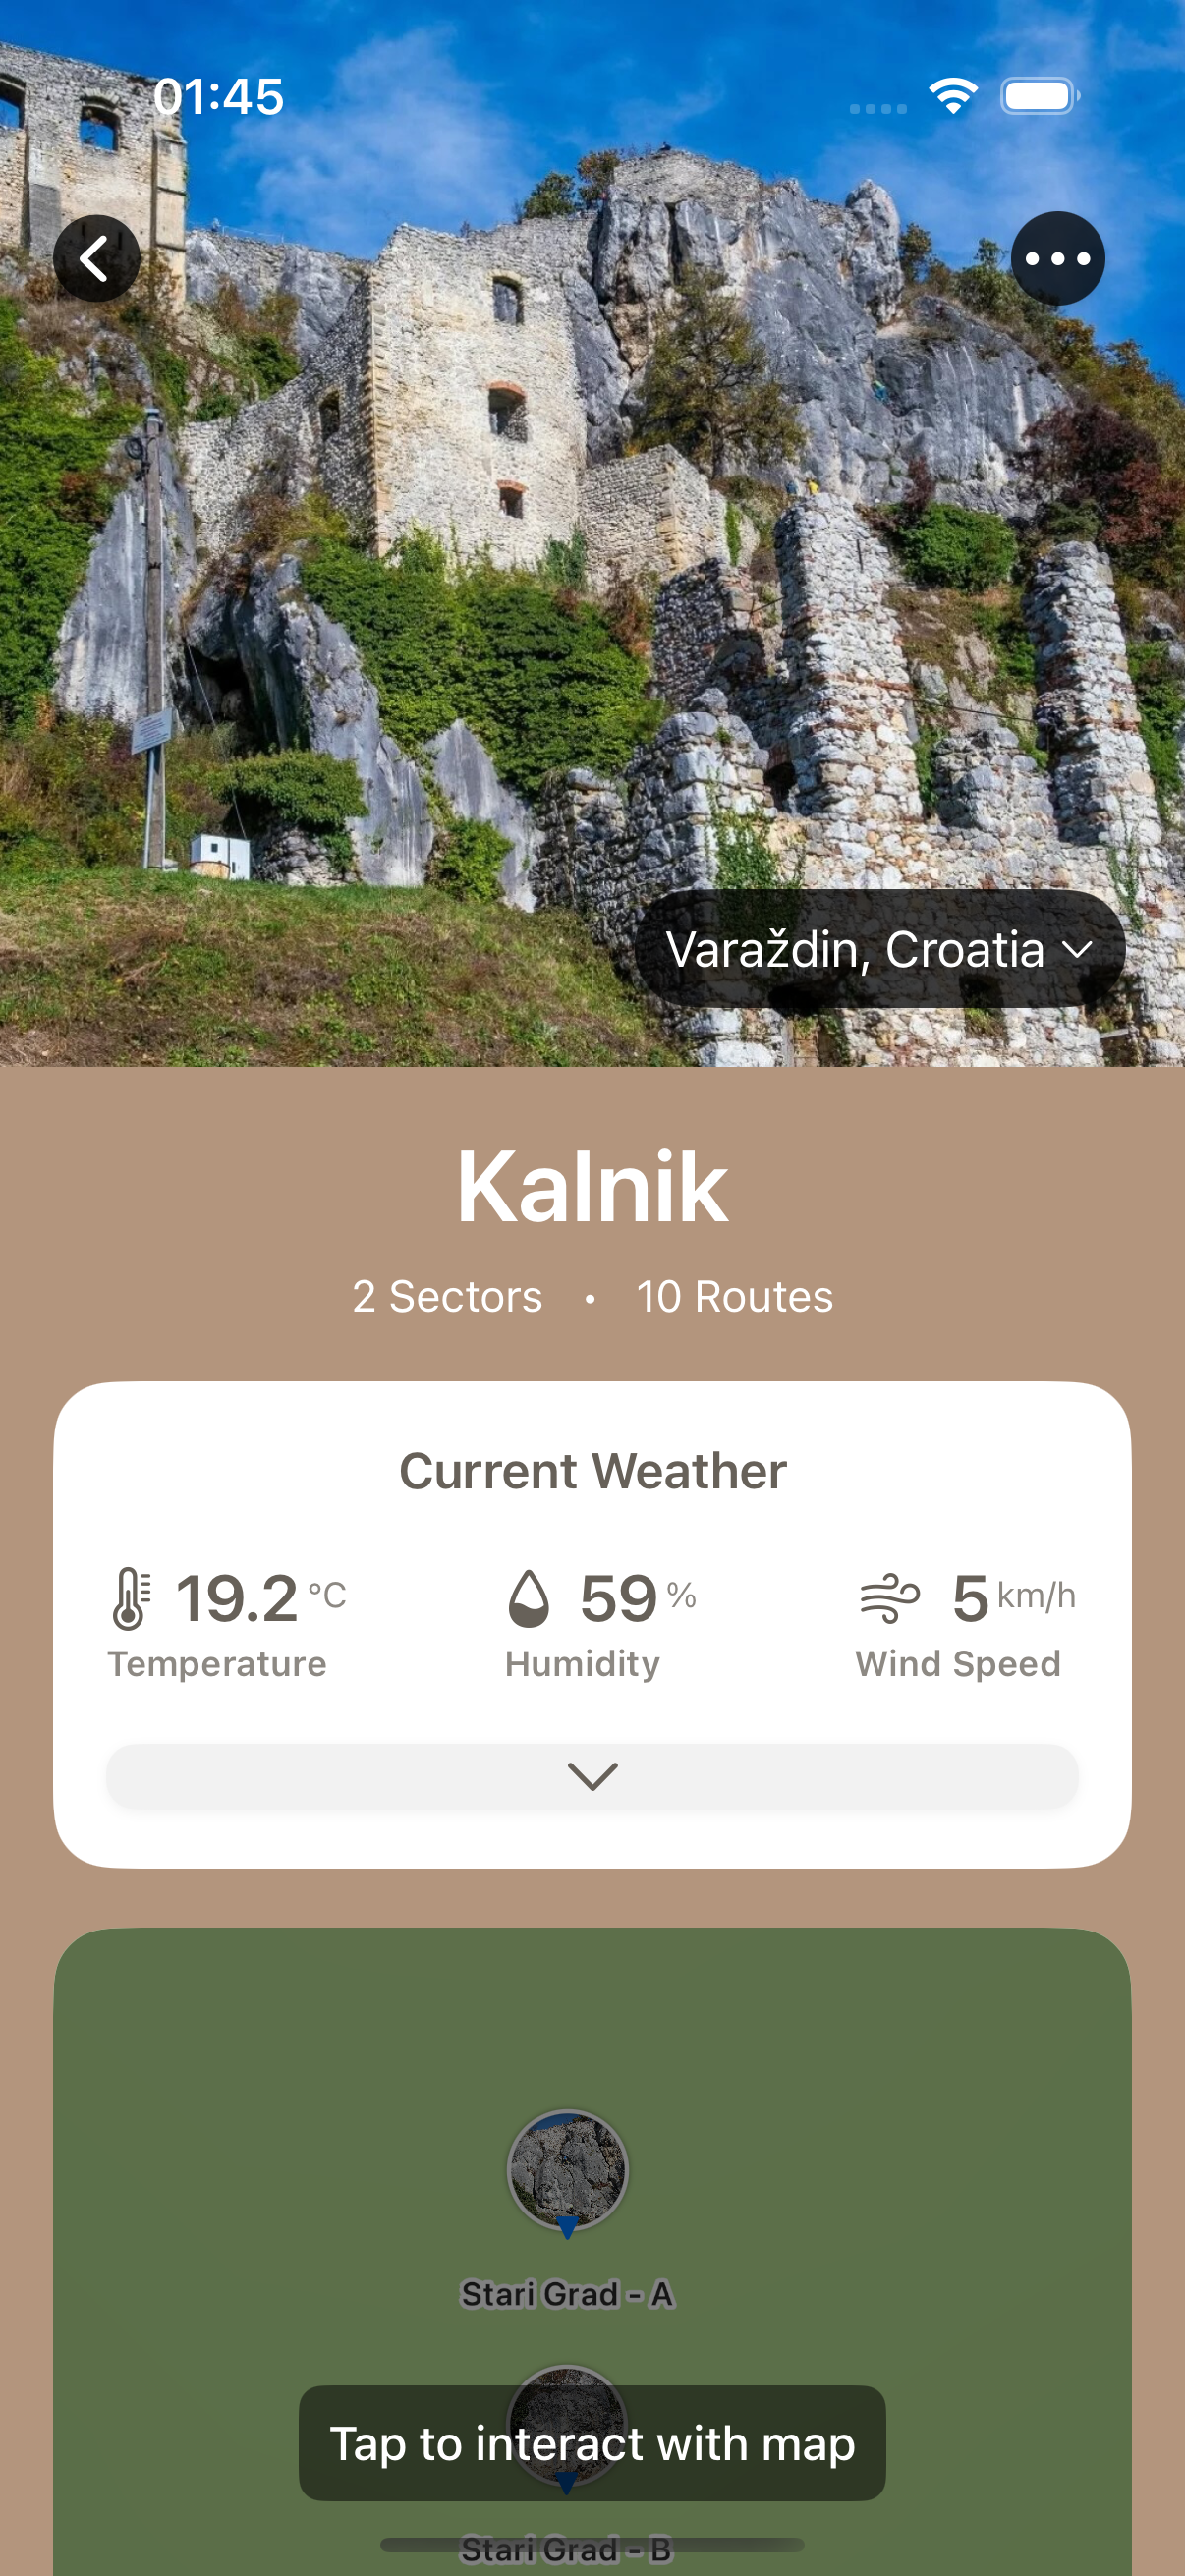
\includegraphics[width=0.3\textwidth]{images/implementacija/crag-details/crag-details-top.png}
        \caption{Mobilna aplikacija}
        \label{fig:detalji_penjališta_mob}
    \end{subfigure}
    \hfill
    \begin{subfigure}[b]{\textwidth}
        \centering
        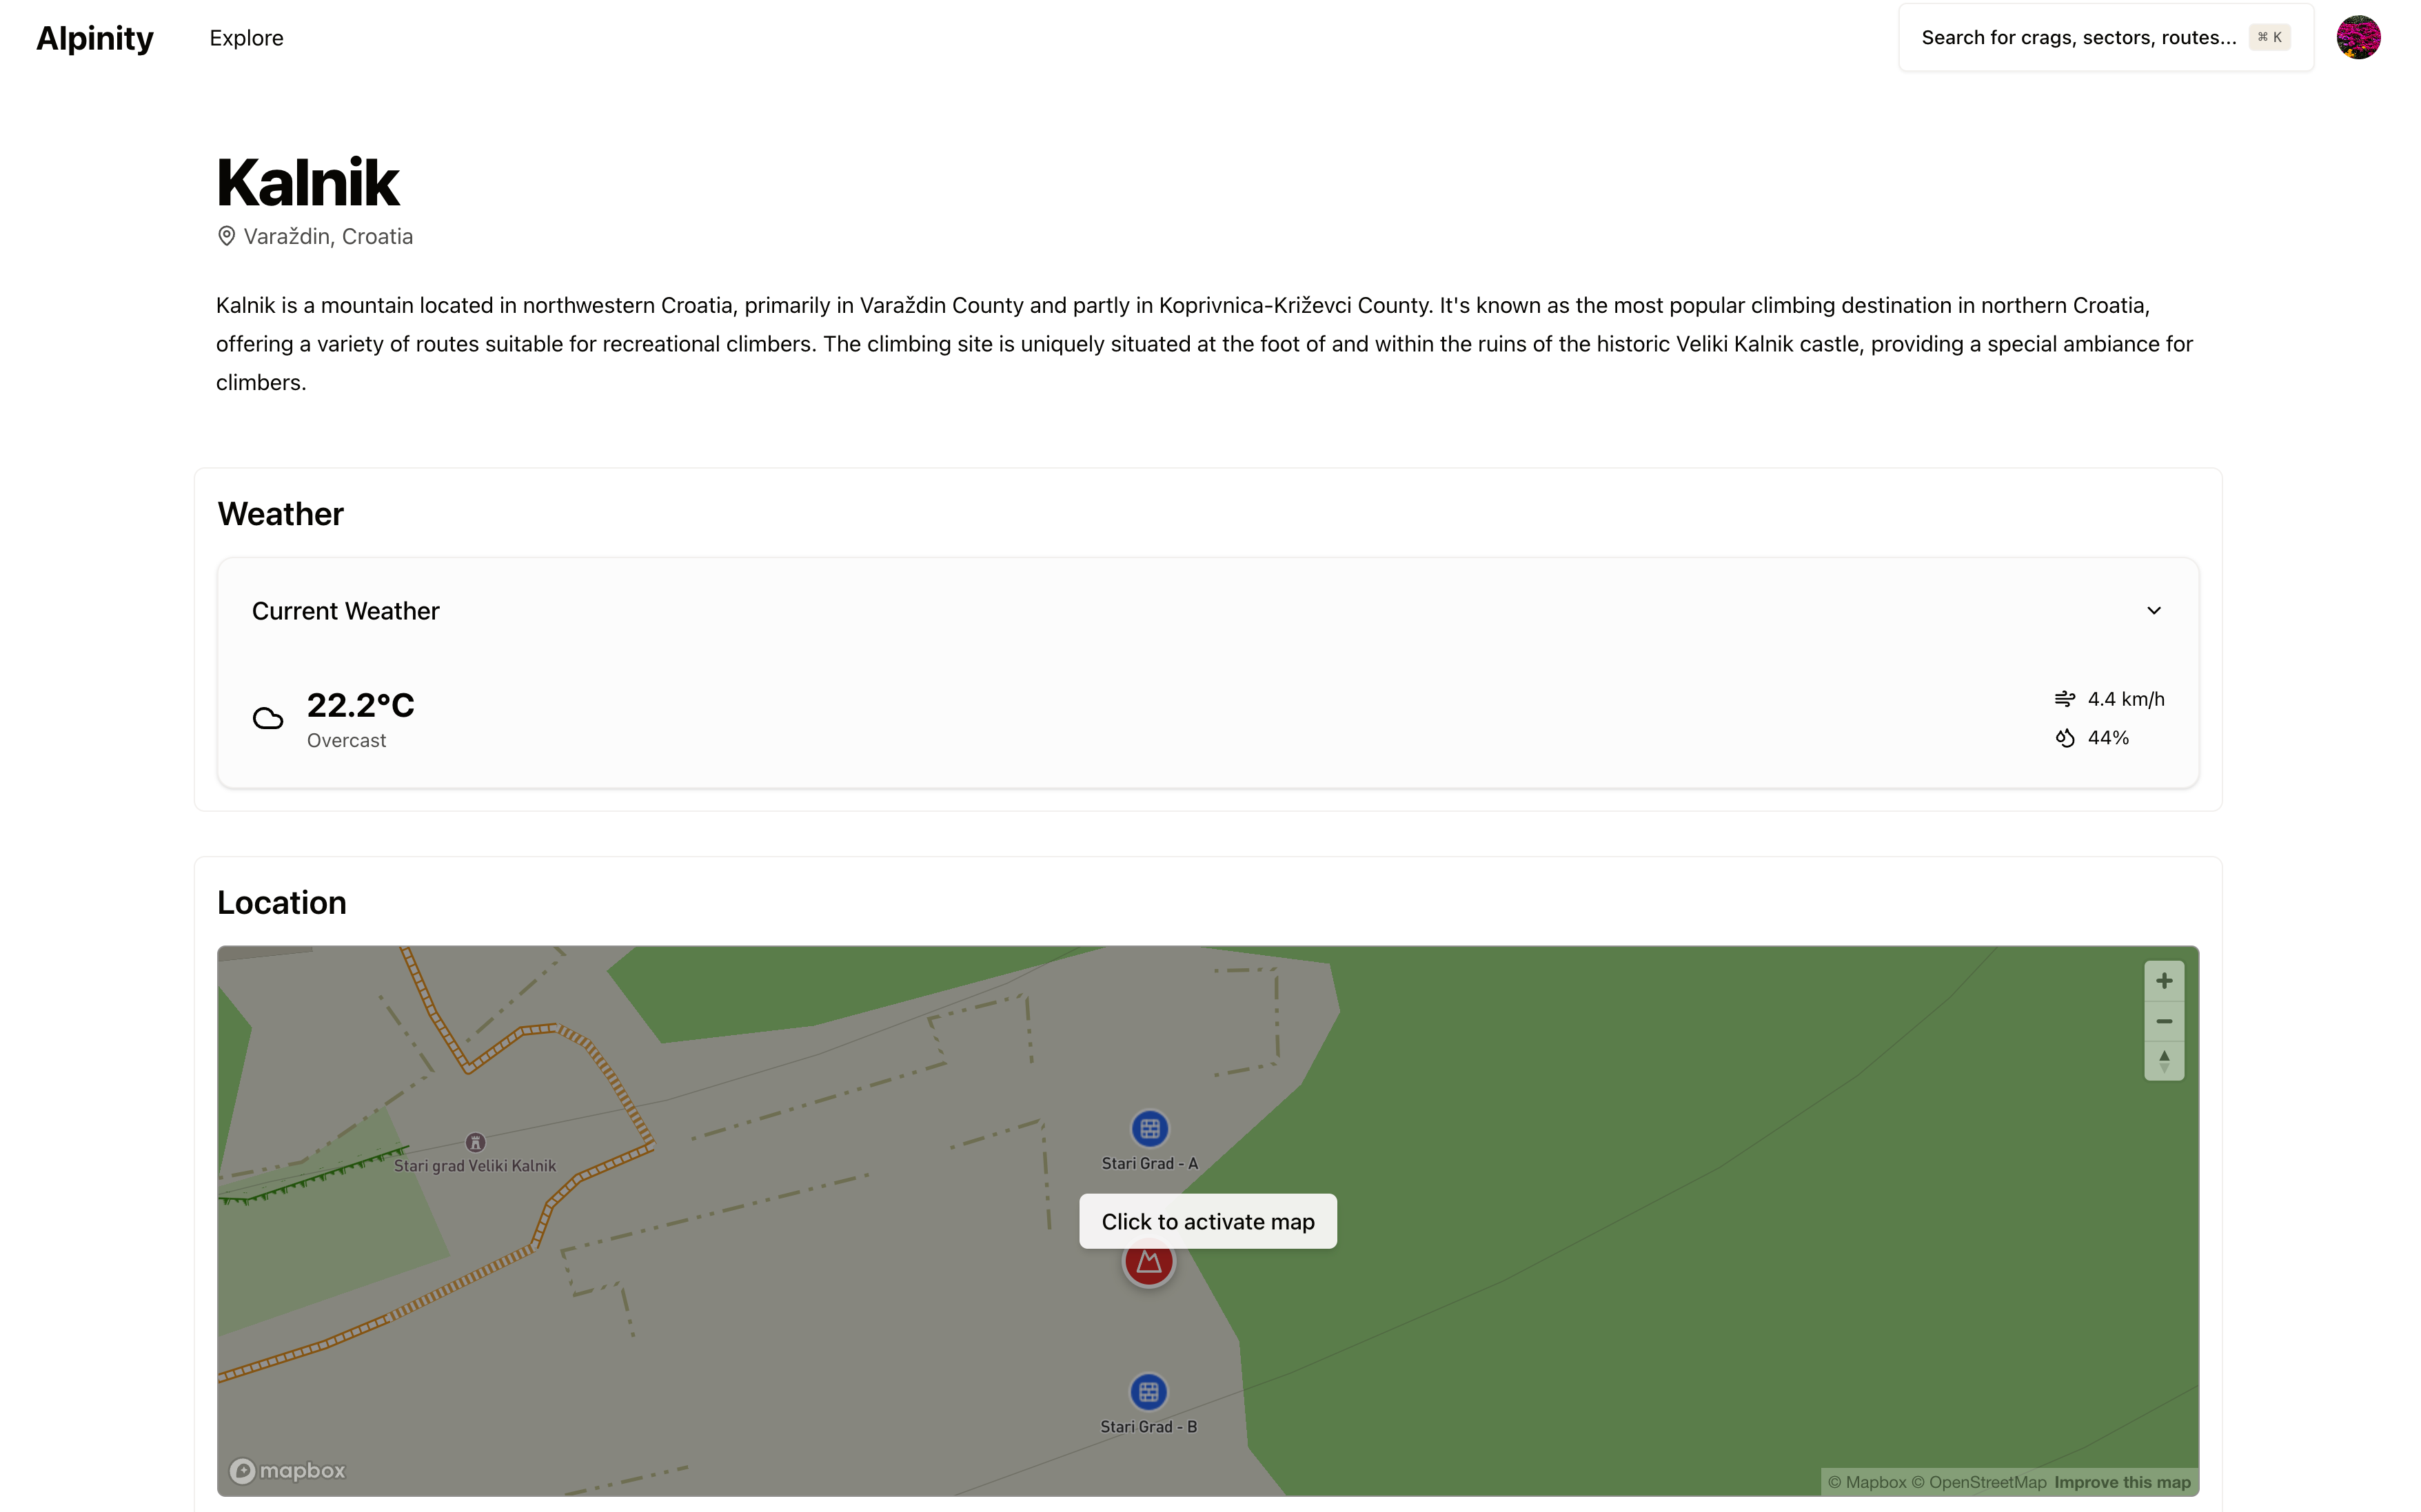
\includegraphics[width=0.9\textwidth]{images/implementacija/web/crag-details/crag-details-top.png}
        \caption{Web aplikacija}
        \label{fig:detalji_penjališta_web}
    \end{subfigure}
    \caption{Detalji penjališta na mobilnoj i web aplikaciji}
    \label{fig:detalji_penjališta_1}
\end{figure}

Odabirom penjališta iz pretrage, s geografske karte ili drugih pregleda, korisnik pristupa zaslonu s detaljnim informacijama o penjalištu (slika~\ref{fig:detalji_penjališta_1}). Zaslon je podijeljen na nekoliko cjelina. Na vrhu se nalazi istaknuta fotografija penjališta, zajedno s nazivom i osnovnim podacima o broju sektora i penjačkih smjerova. 
Na web aplikaciji nalazi se isti prikaz, ali s manjim promjenama. Slika penjališta nalazi se ispod geografske karte, a broj sektora i penjačkih smjerova nalazi se u prikazu sektora i penjačkih smjerova.

\begin{figure}[H]
    \centering
    \begin{subfigure}[b]{\textwidth}
        \centering
        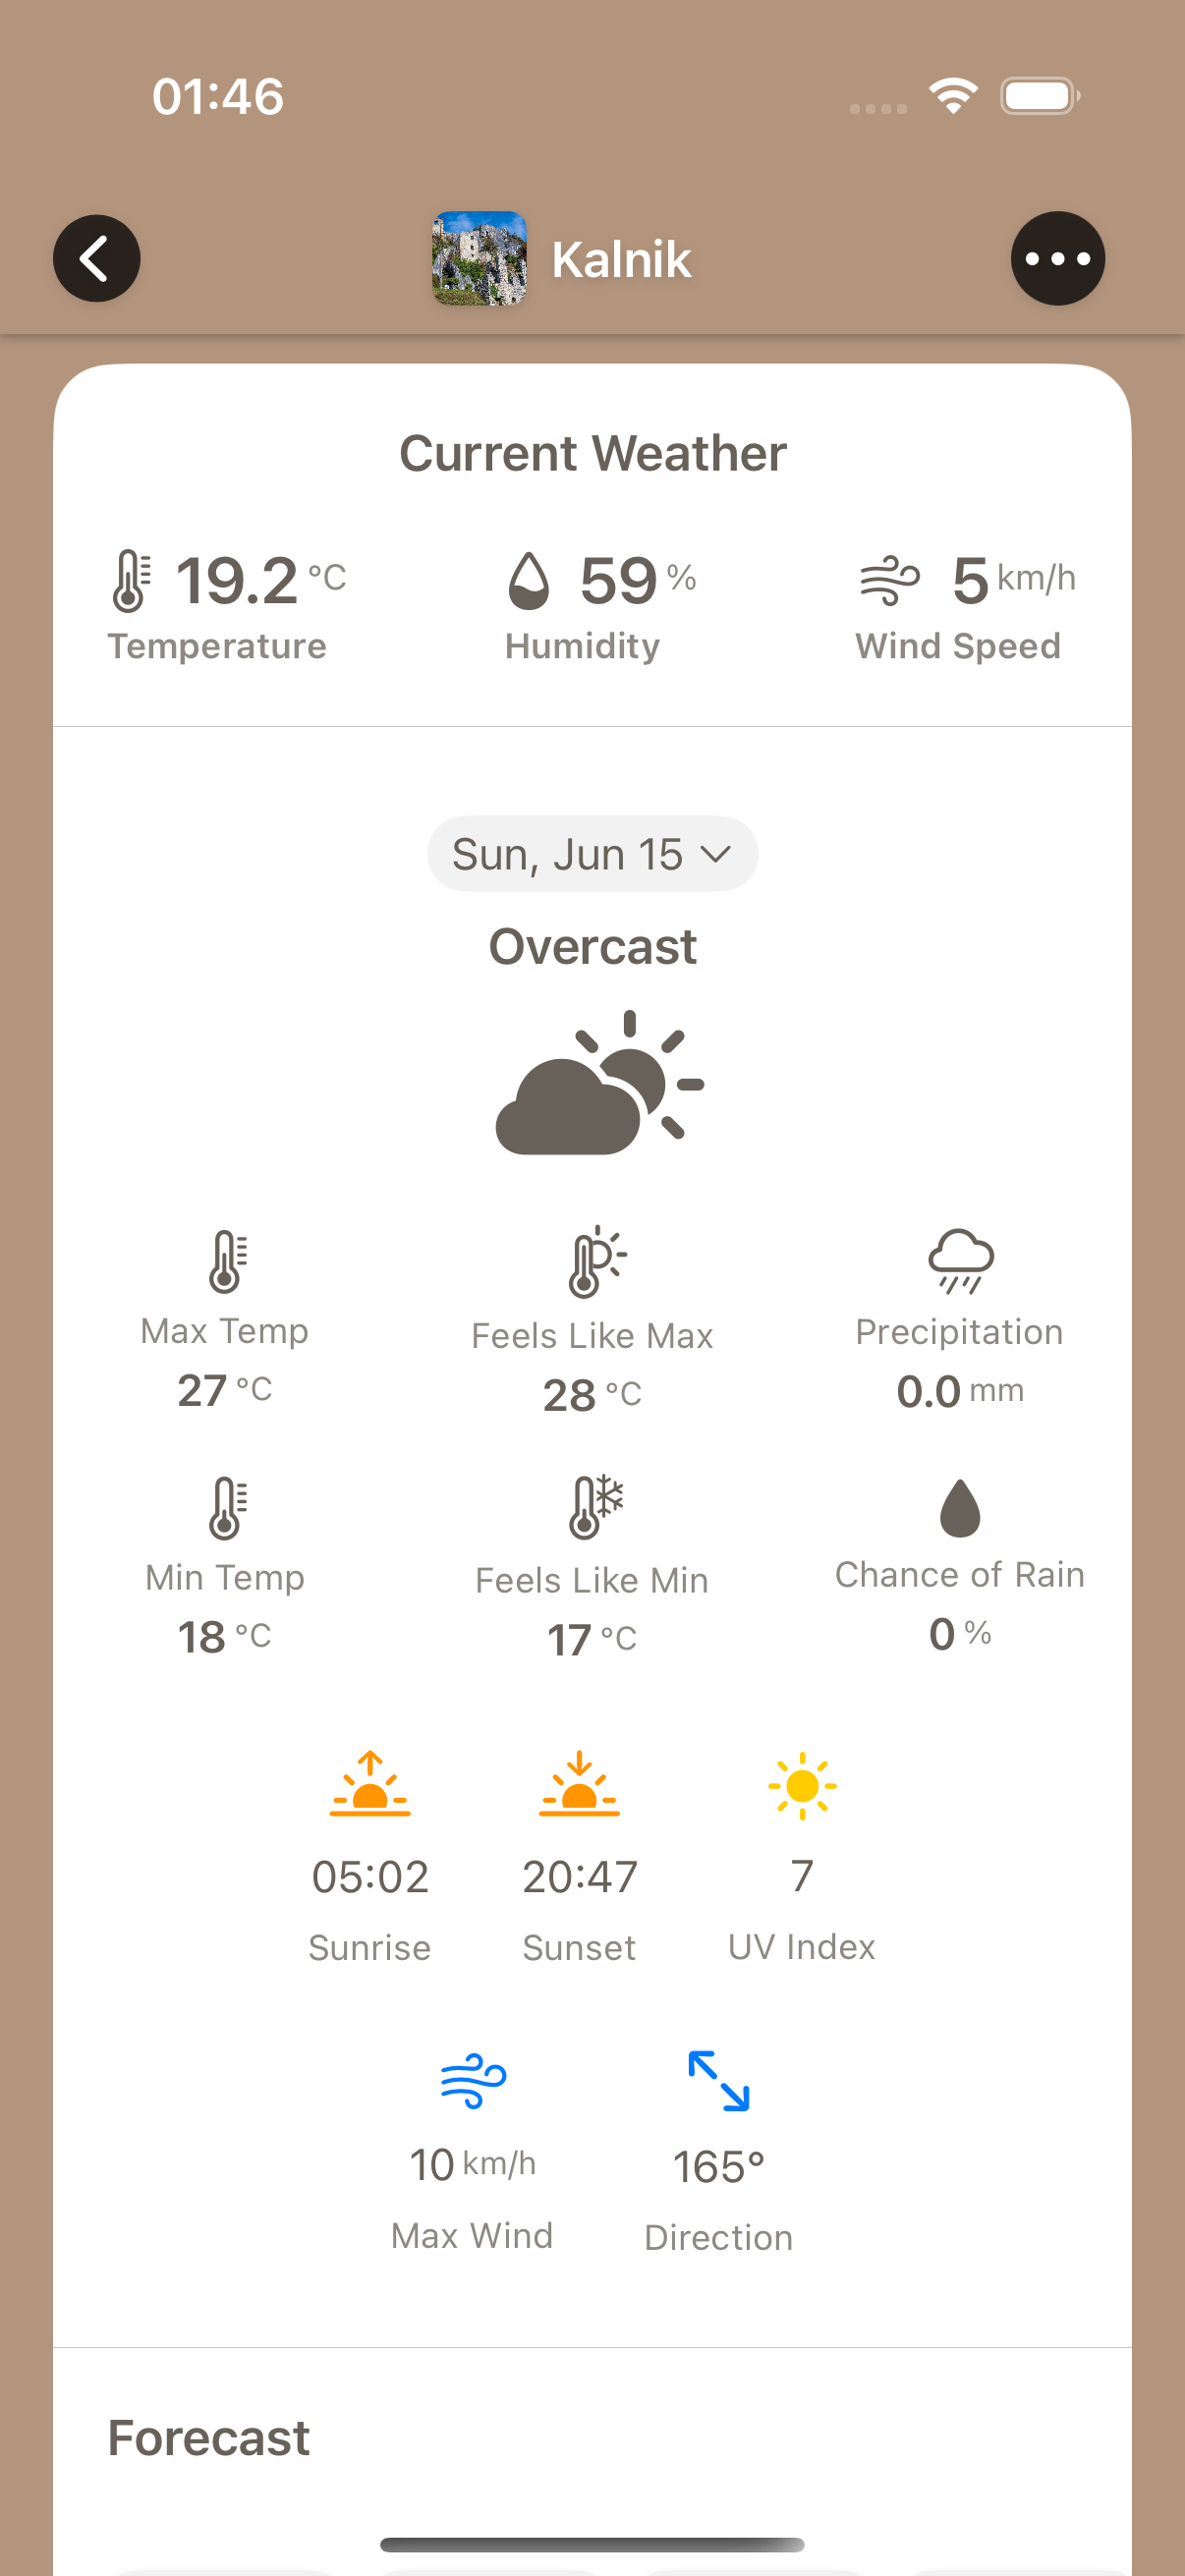
\includegraphics[width=0.35\textwidth]{images/implementacija/crag-details/crag-weather-1.png}
        \caption{Mobilna aplikacija}
        \label{fig:vremenska_prognoza_mob}
    \end{subfigure}
    \hfill
    \begin{subfigure}[b]{\textwidth}
        \centering
        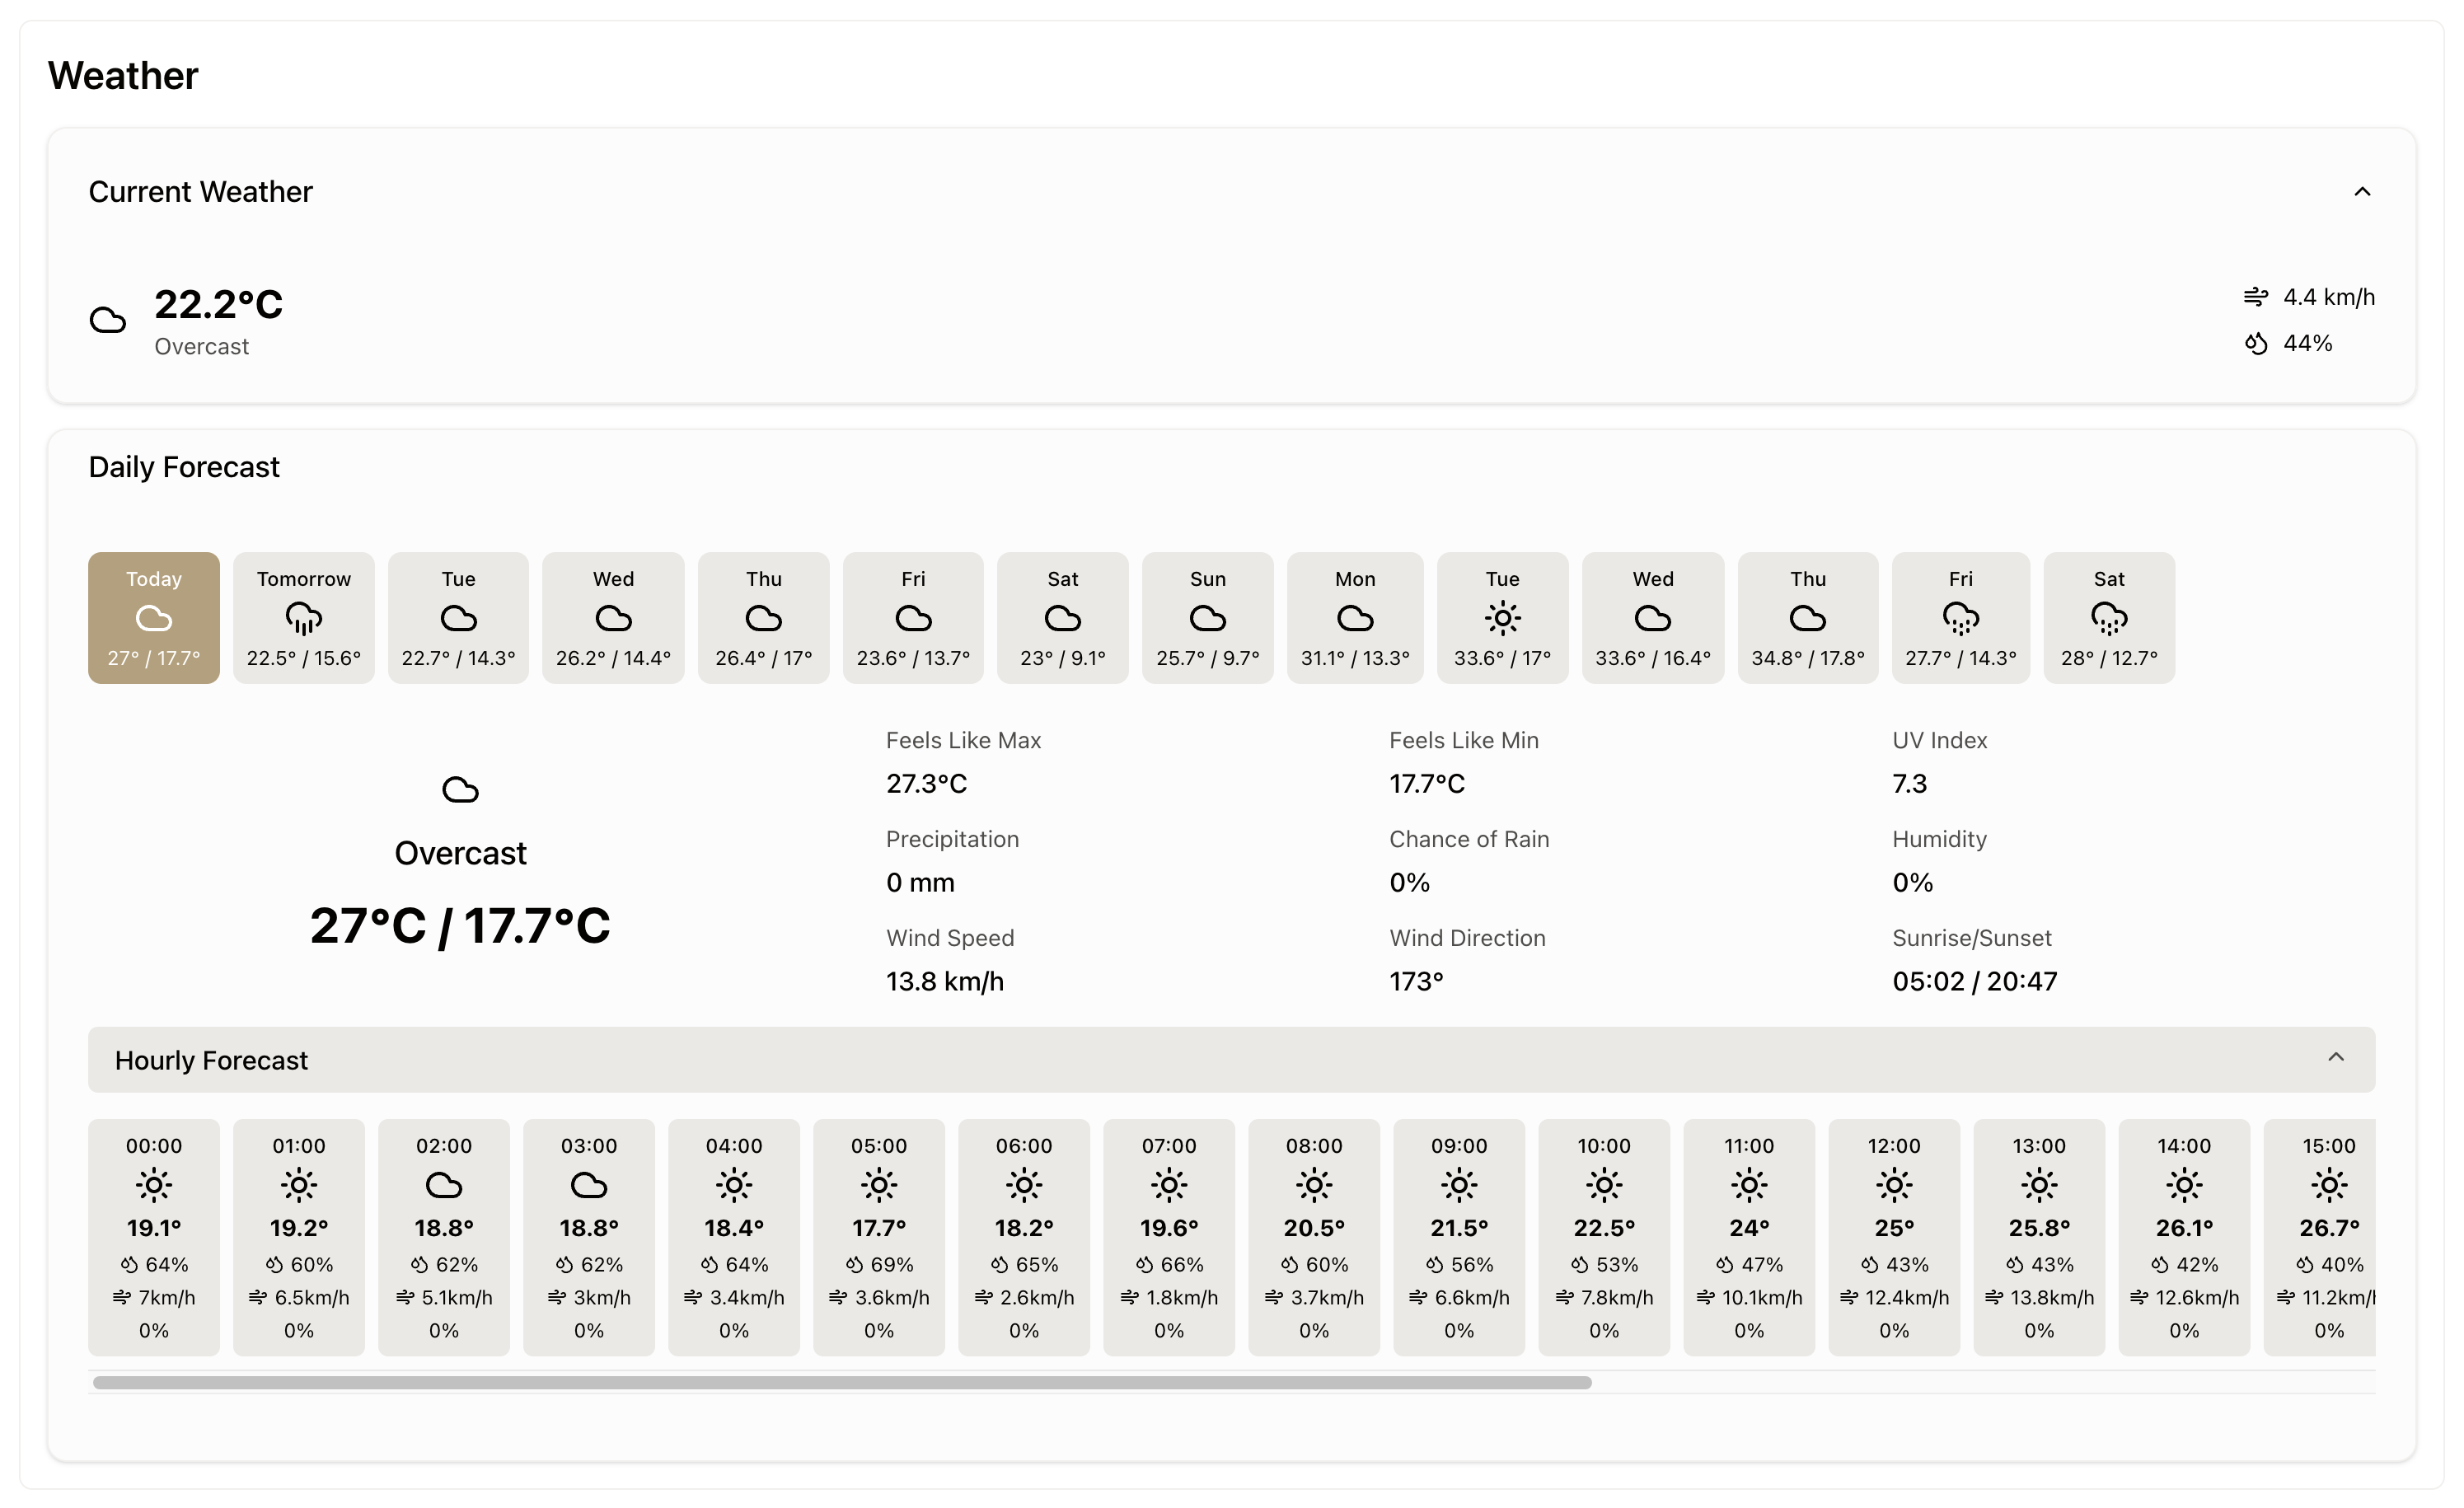
\includegraphics[width=0.9\textwidth]{images/implementacija/web/crag-details/crag-weather.png}
        \caption{Web aplikacija}
        \label{fig:vremenska_prognoza_web}
    \end{subfigure}
    \caption{Vremenska prognoza na mobilnoj i web aplikaciji}
    \label{fig:vremenska_prognoza}
\end{figure}

Odmah ispod, nalazi se komponenta s vremenskom prognozom (slika~\ref{fig:vremenska_prognoza}). Ona prikazuje trenutne vremenske uvjete, kao i detaljnu prognozu po satima za sljedećih 14 dana. Detaljna prognoza uključuje temperaturu, vjerojatnost i količina padalina, brzinu vjetra, UV indeks i ostale relevantne podatke. Ova funkcionalnost je važna za planiranje penjačkih izleta.


Nakon komponente vremenske prognoze sljedi interaktivna karta penjališta koja prikazuje precizne lokacije svih sektora, omogućujući korisniku lako snalaženje i planiranje kretanja između njih (slika~\ref{fig:interaktivna_karta}). 

\begin{figure}[H]
    \centering
    \begin{subfigure}[b]{\textwidth}
        \centering
        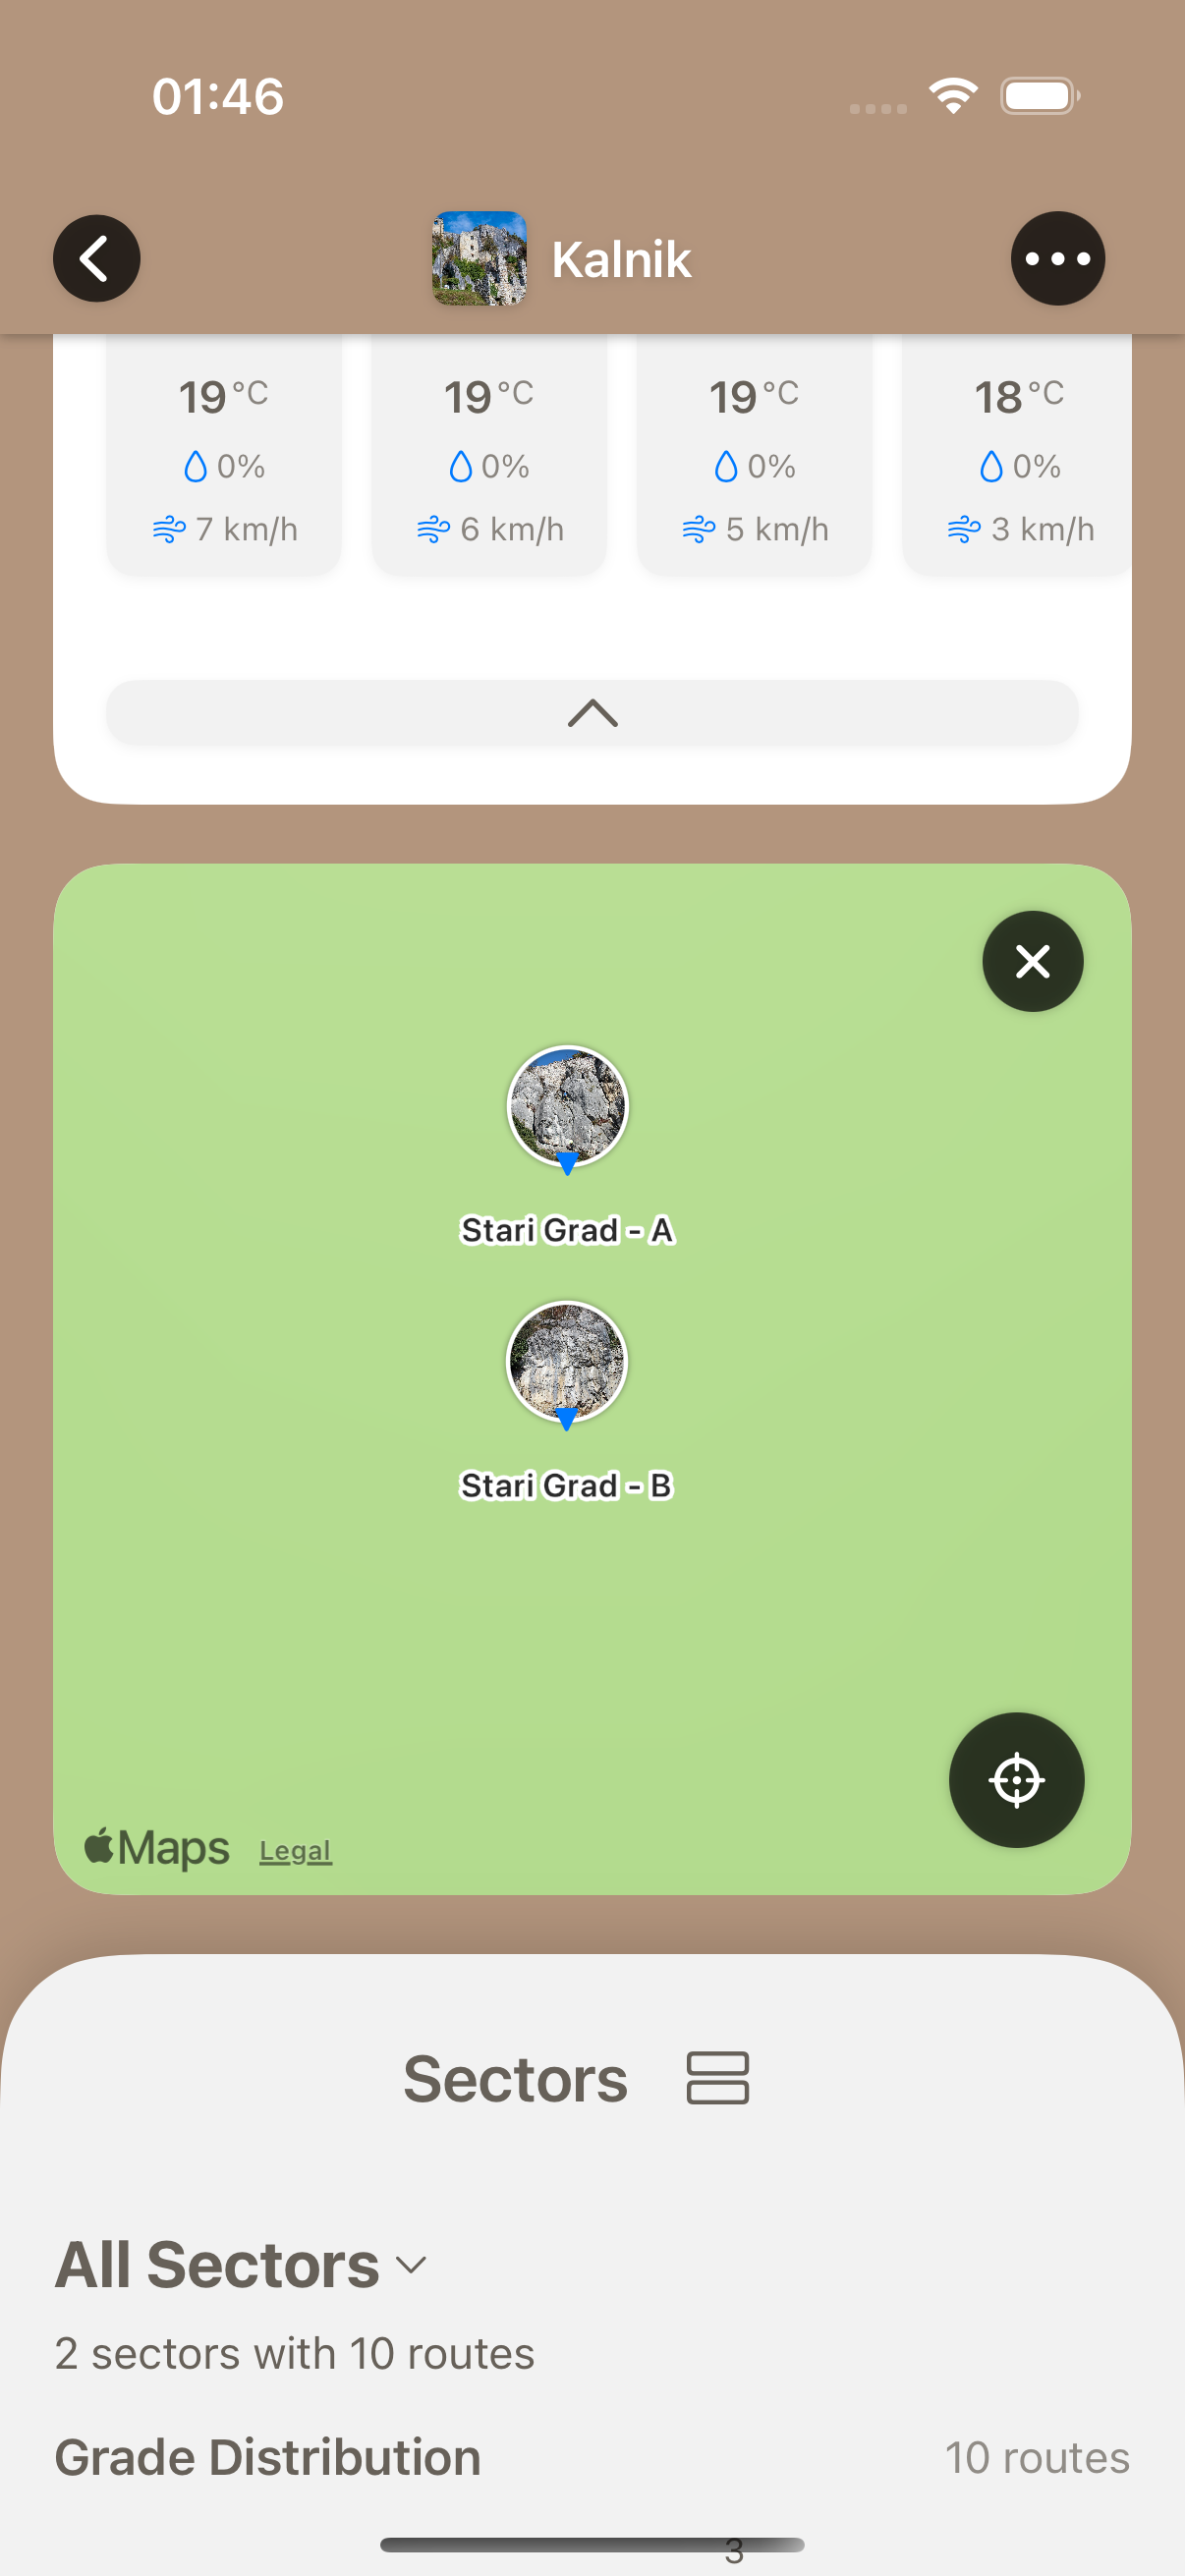
\includegraphics[width=0.35\textwidth]{images/implementacija/crag-details/crag-map.png}
        \caption{Mobilna aplikacija}
        \label{fig:interaktivna_karta_mob}
    \end{subfigure}
    \hfill
    \begin{subfigure}[b]{\textwidth}
        \centering
        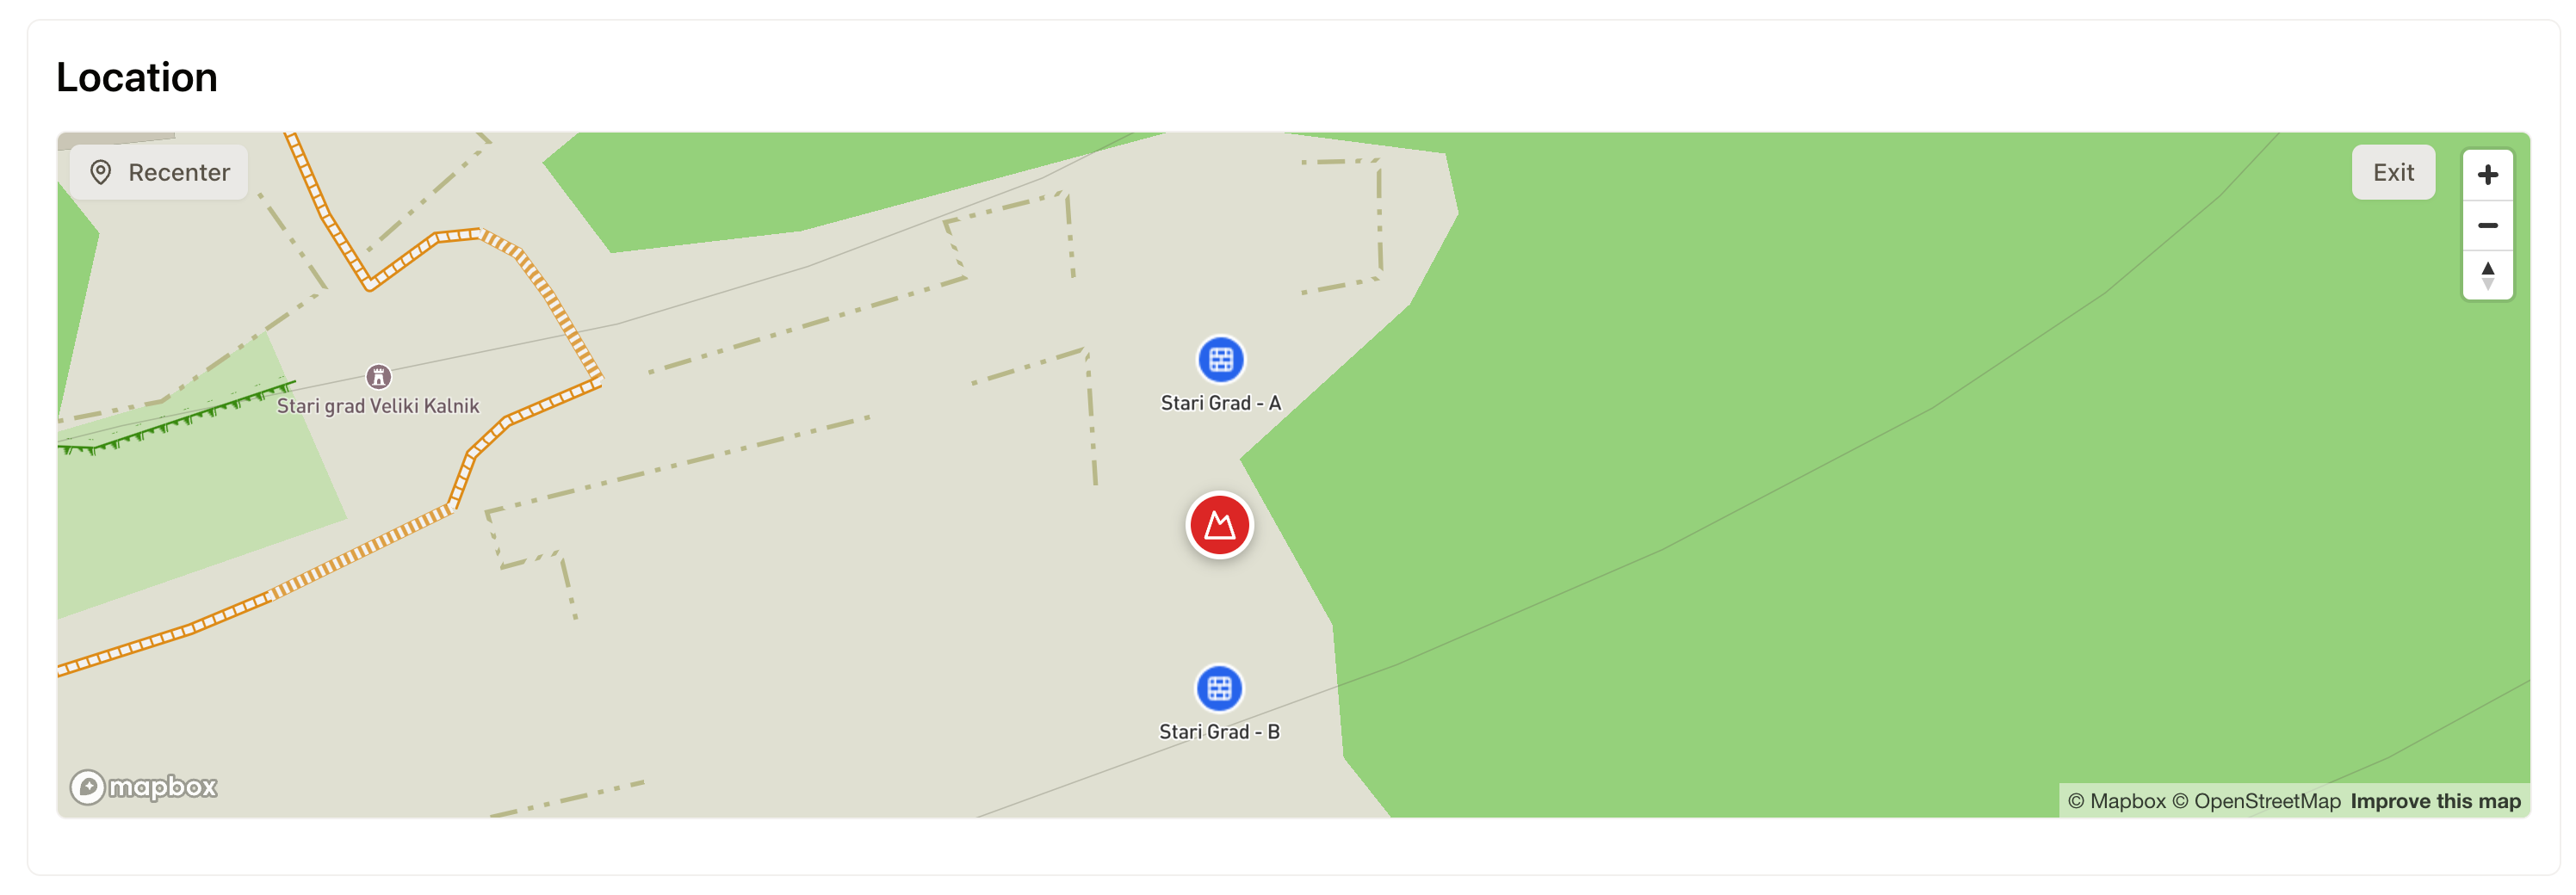
\includegraphics[width=0.9\textwidth]{images/implementacija/web/crag-details/crag-map.png}
        \caption{Web aplikacija}
        \label{fig:interaktivna_karta_web}
    \end{subfigure}
    \caption{Interaktivna karta penjališta}
    \label{fig:interaktivna_karta}
\end{figure}

Ispod karte nalazi se prikaz detalja za sektore. Prije ikakvih odabira, korisniku se prikazuje popis svih penjačkih smjerova grupiranih po sektorima te distribucija težina na penjalištu (slika~\ref{fig:prikaz_detalja_za_sektore}). 

\begin{figure}[H]
    \centering
    \begin{subfigure}[b]{0.4\textwidth}
        \centering
        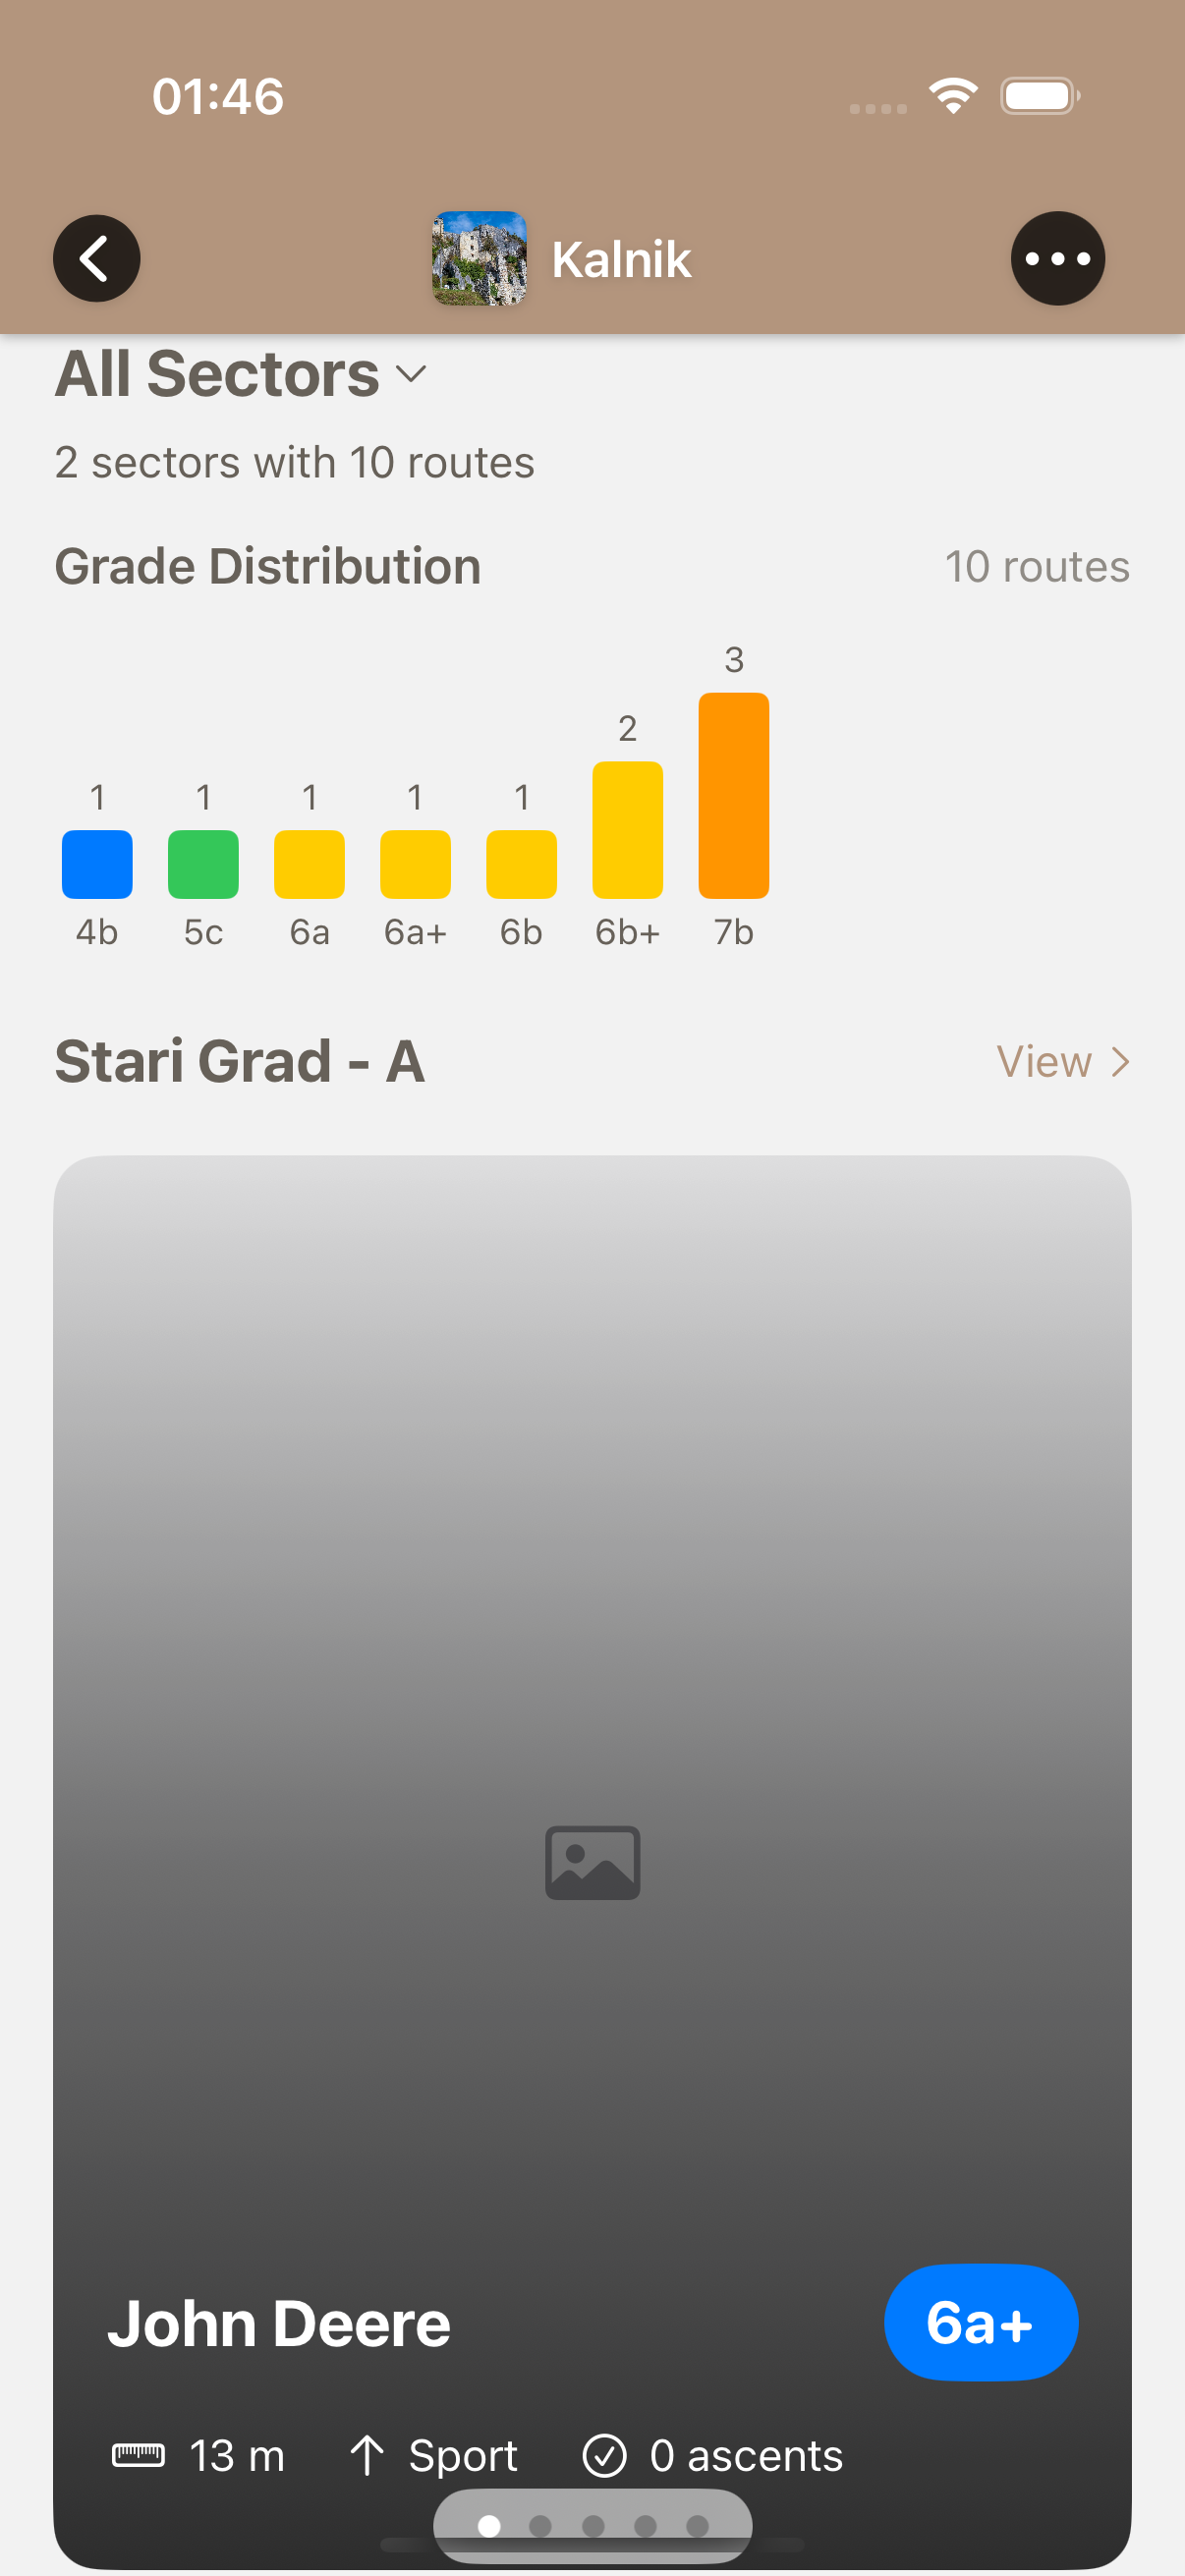
\includegraphics[width=0.7\textwidth]{images/implementacija/crag-details/crag-all-sectors-tabs.png}
        \caption{Mobilna aplikacija}
        \label{fig:prikaz_detalja_za_sektore_mob}
    \end{subfigure}
    \hfill
    \begin{subfigure}[b]{0.55\textwidth}
        \centering
        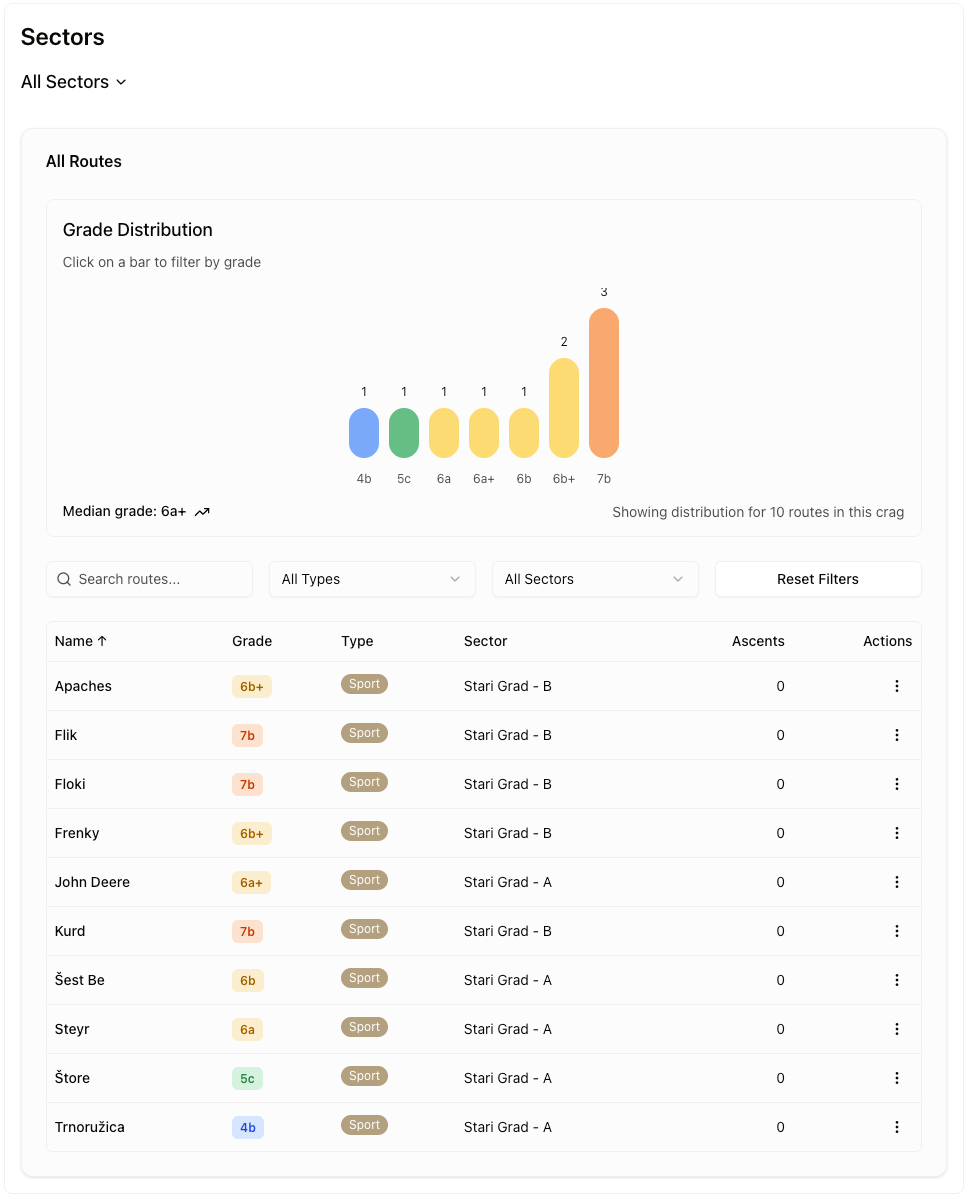
\includegraphics[width=1\textwidth]{images/implementacija/web/crag-details/crag-all-sectors.png}
        \caption{Web aplikacija}
        \label{fig:prikaz_detalja_za_sektore_web}
    \end{subfigure}
    \caption{Prikaz detalja za sektore}
    \label{fig:prikaz_detalja_za_sektore}
\end{figure}

Klikom na određenu težinu u grafu filtriraju se svi penjački smjerovi koji pripadaju odabranoj težini. Lista penjačkih smjerova na mobilnoj aplikaciji je horizontalna lista koja prikazuje penjački smjer u većem formatu kako bi se mogla bolje vidjeti slika penjačkog smjera. Preko slike nalaze se detalji o penjačkom smjeru poput naziva, težine, dužine, tipa i broja uspona.

\begin{figure}[H]
    \centering
    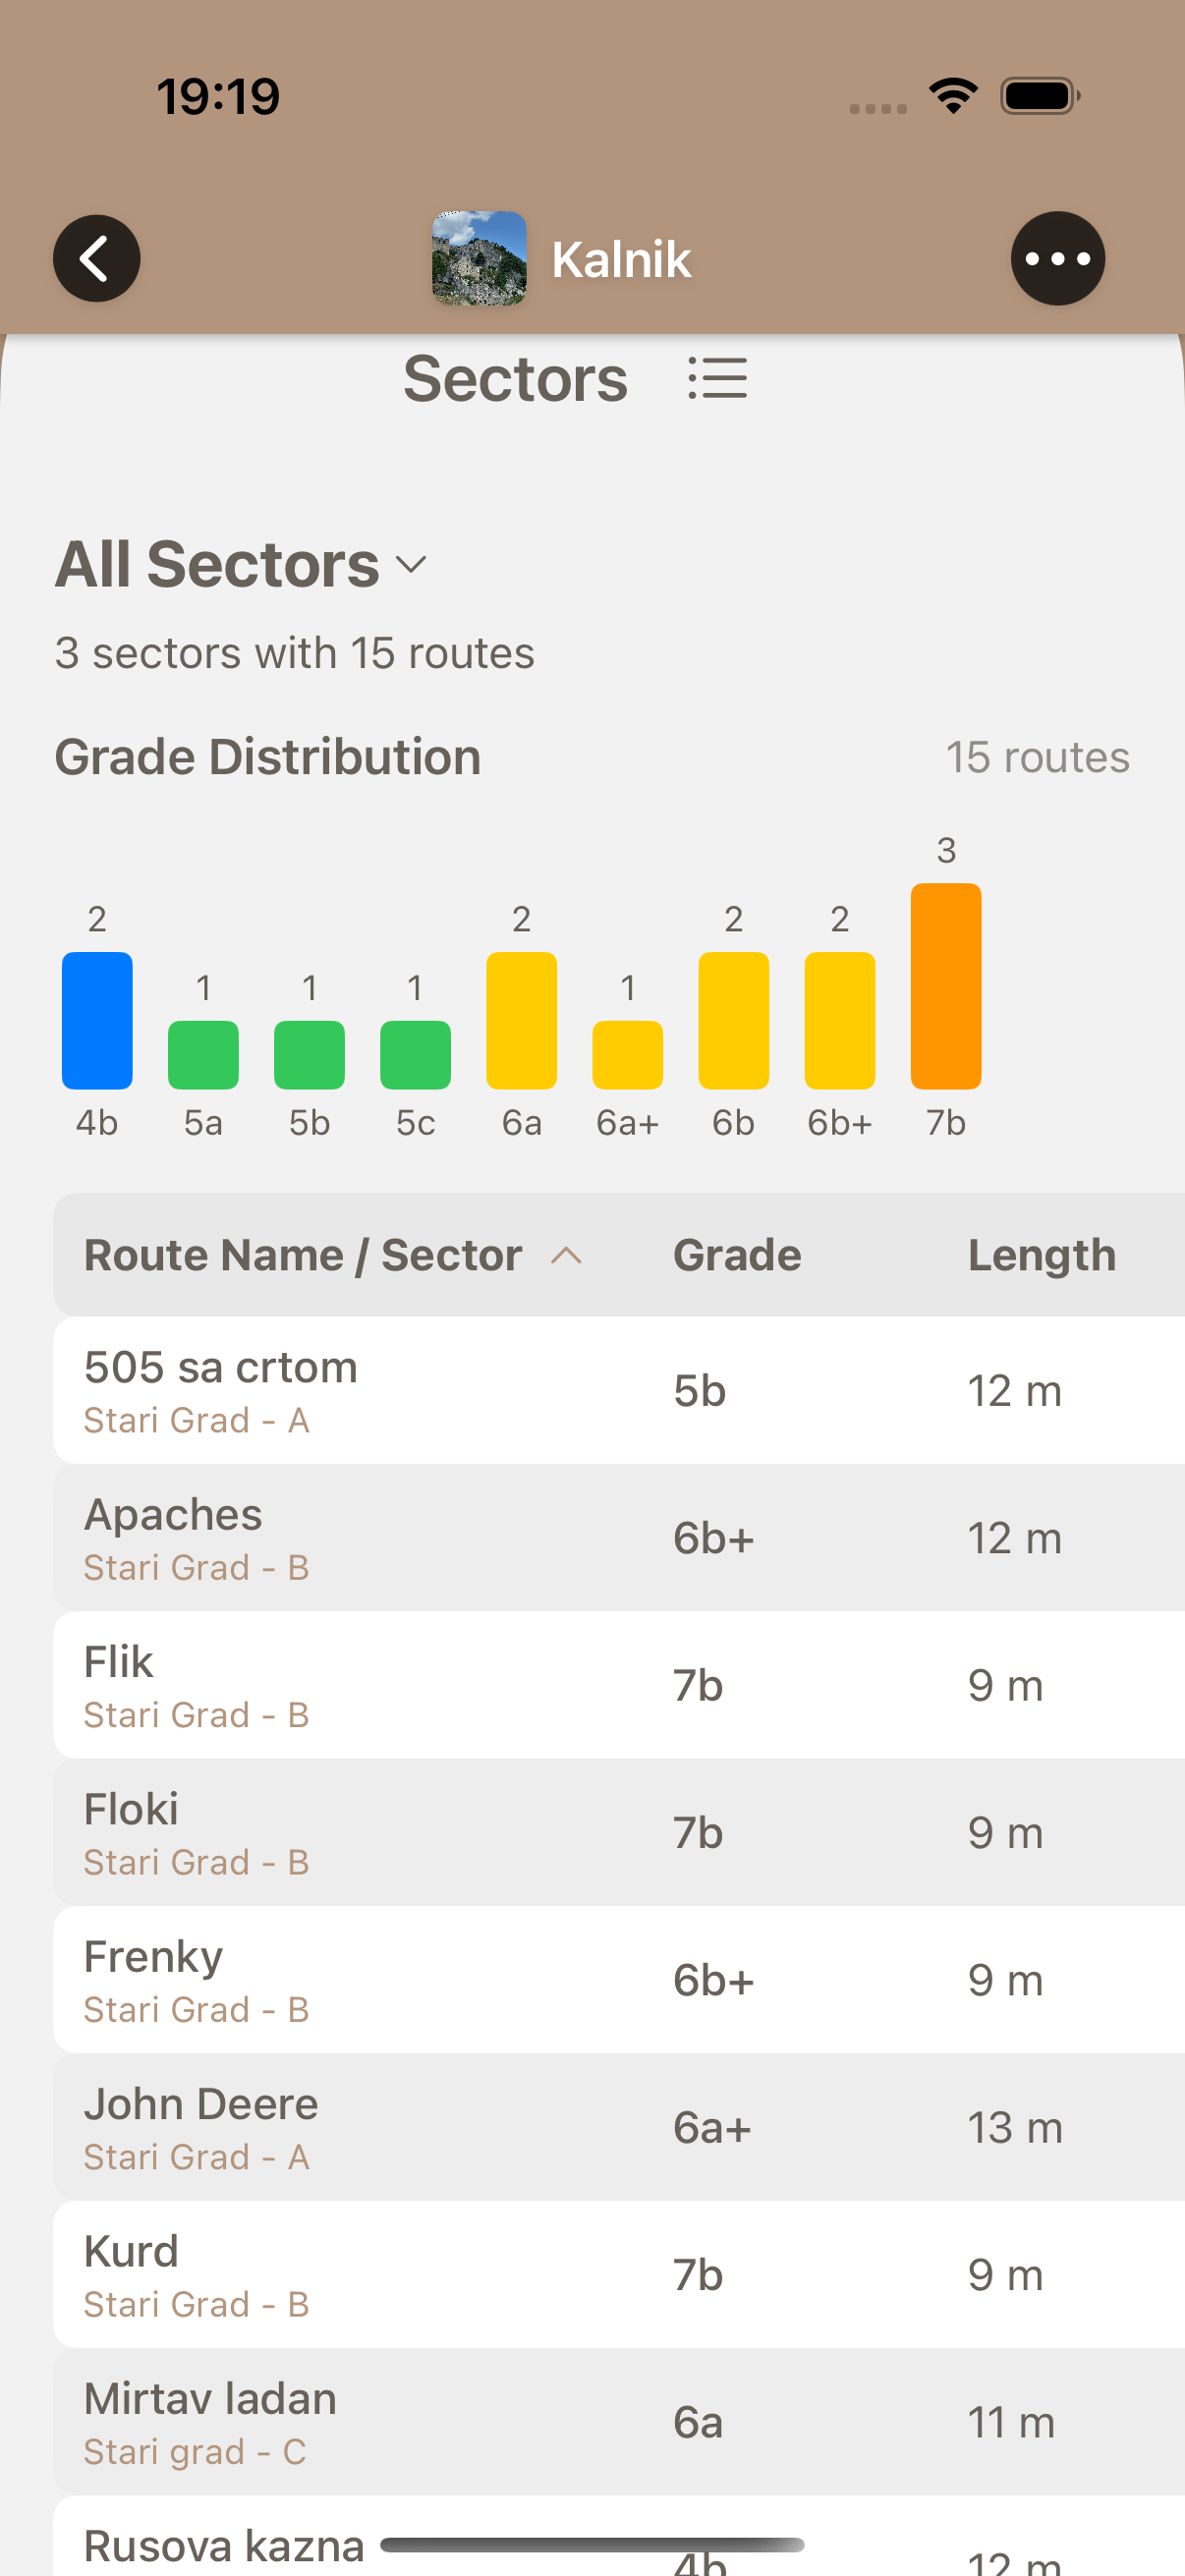
\includegraphics[width=0.35\textwidth]{images/implementacija/crag-details/crag-all-sectors-table.png}
    \caption{Tablični prikaz sektora na mobilnoj aplikaciji}
    \label{fig:tablični_prikaz_sektora}
\end{figure}

Ako korisnik preferira tablični prikaz na mobilnoj aplikaciji, može to promijeniti klikom na gumb pored naslova "Sektori" (eng. \textit{Sectors}) (slika~\ref{fig:tablični_prikaz_sektora}). Na web aplikaciji tablični prikaz je zadani prikaz. Tablični prikaz omogućuje pregled svih penjačkih smjerova te sortiranje po nazivu, težini, dužini, tipu te broju uspona. S obzirom da na web aplikaciji nije grupiran prikaz po sektorima, postoje filteri koji korisnik može koristiti za filtriranje penjačkih smjerova po imenu, tipu i sektoru.

Klikom na izbornik "Svi sektori" (eng. \textit{All sectors}) korisniku prikazuje se popis svih sektora na penjalištu (slika~\ref{fig:prikaz_detalja_za_odabrani_sektor}). 

\begin{figure}[H]
    \centering
    \begin{subfigure}[b]{0.35\textwidth}
        \centering
        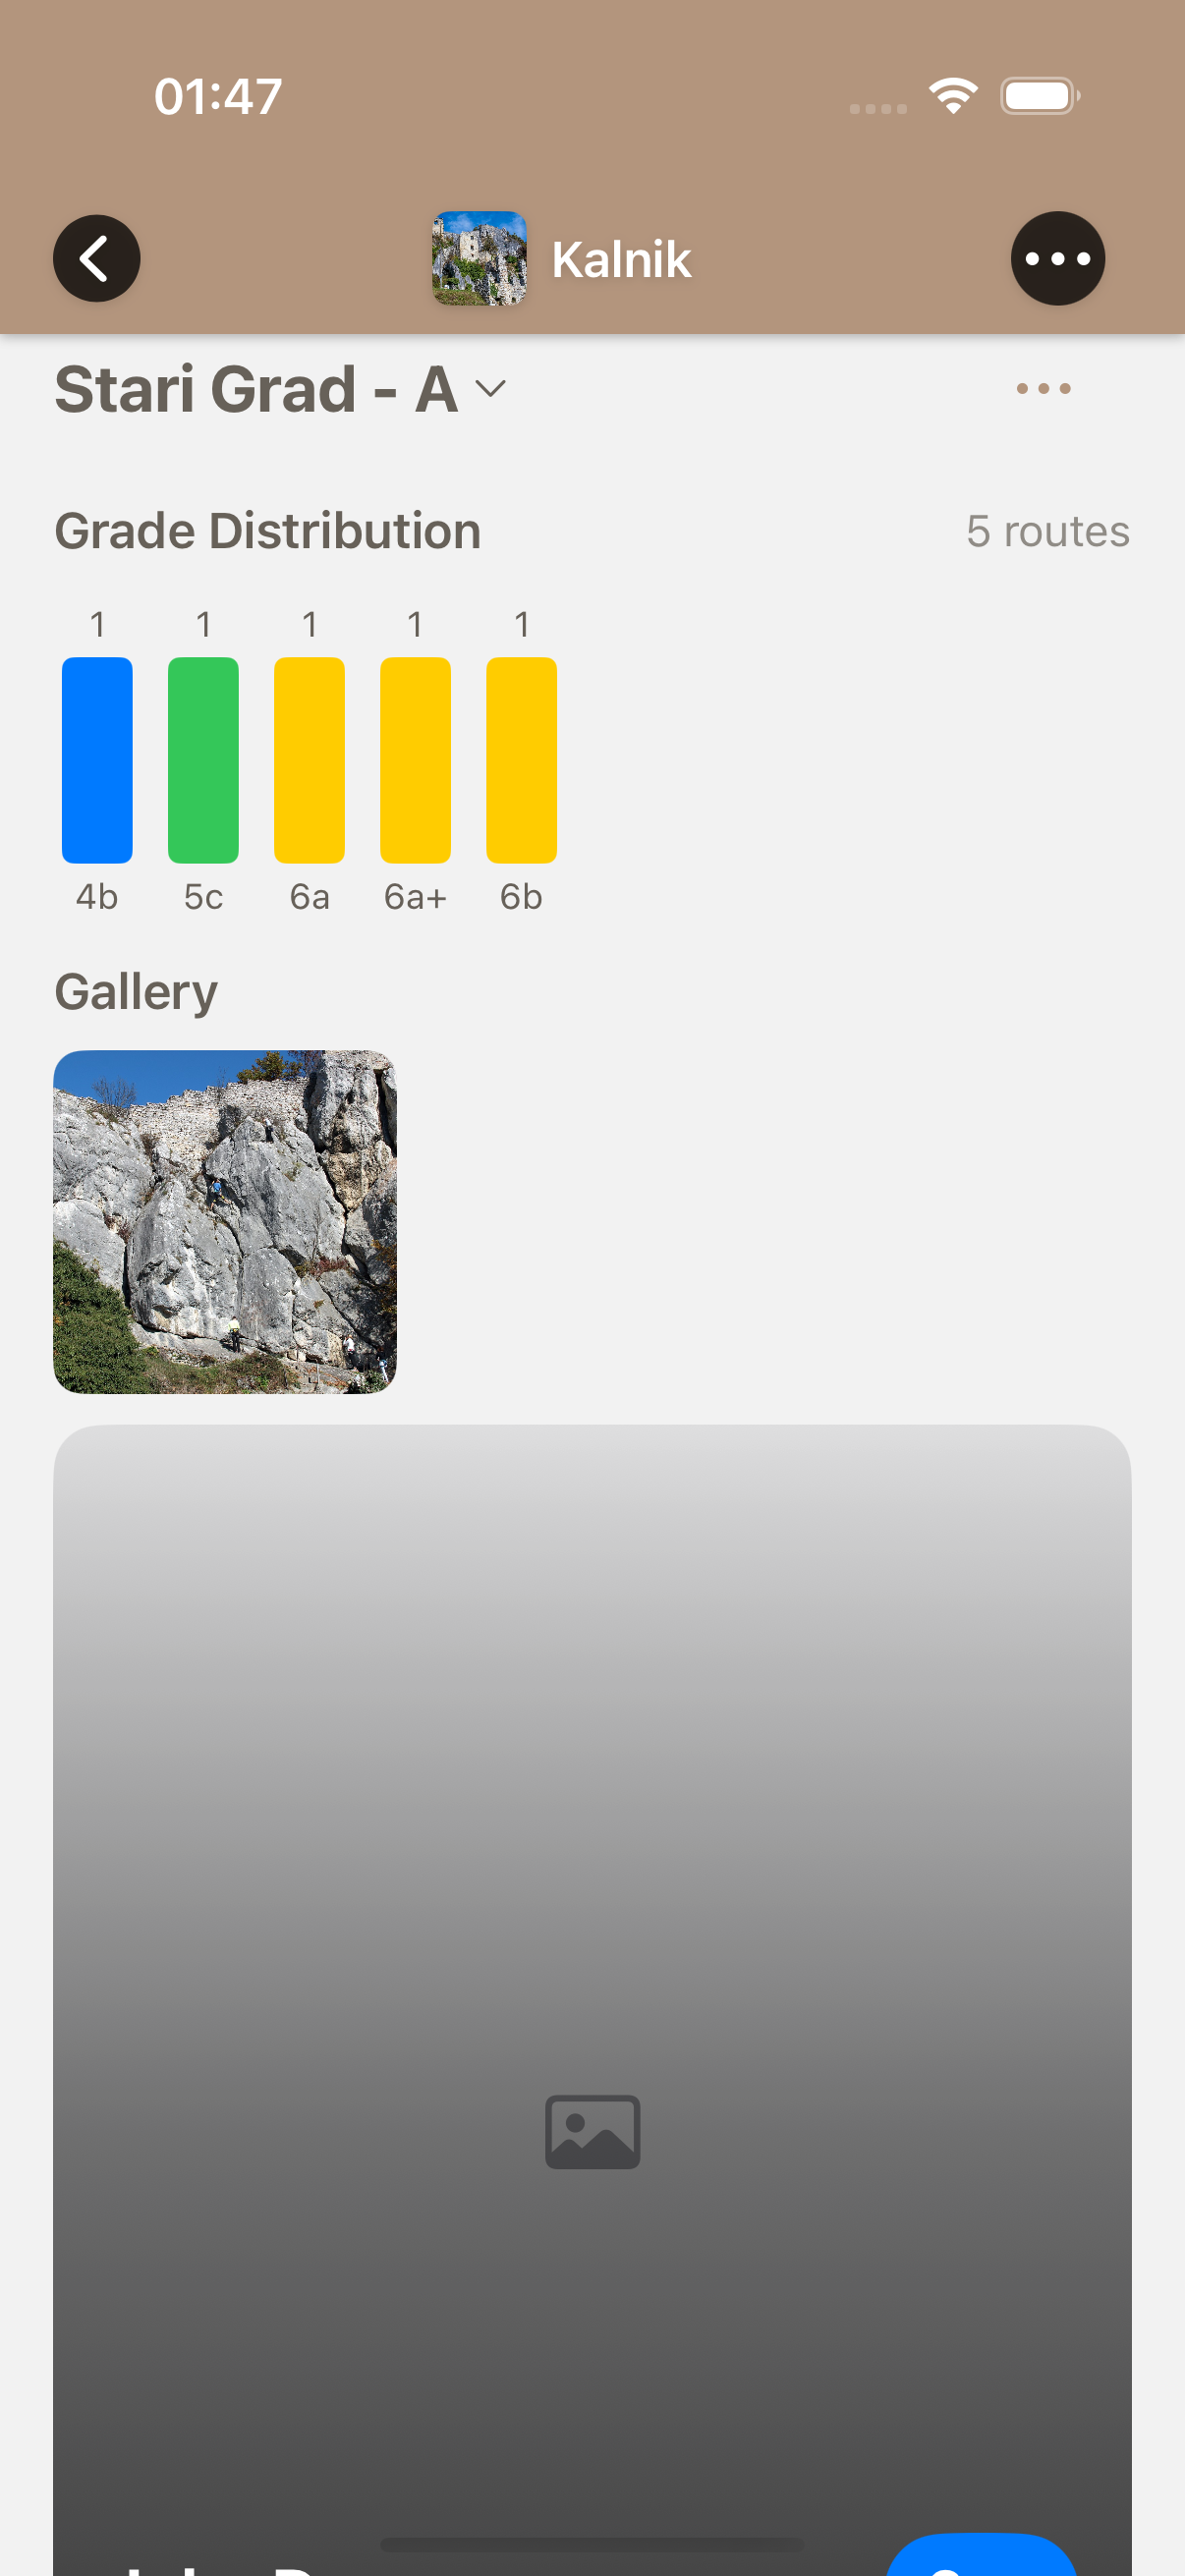
\includegraphics[width=\textwidth]{images/implementacija/crag-details/crag-selected-sector.png}
        \caption{Mobilna aplikacija}
        \label{fig:prikaz_detalja_za_odabrani_sektor_mob}
    \end{subfigure}
    \hfill
    \begin{subfigure}[b]{0.6\textwidth}
        \centering
        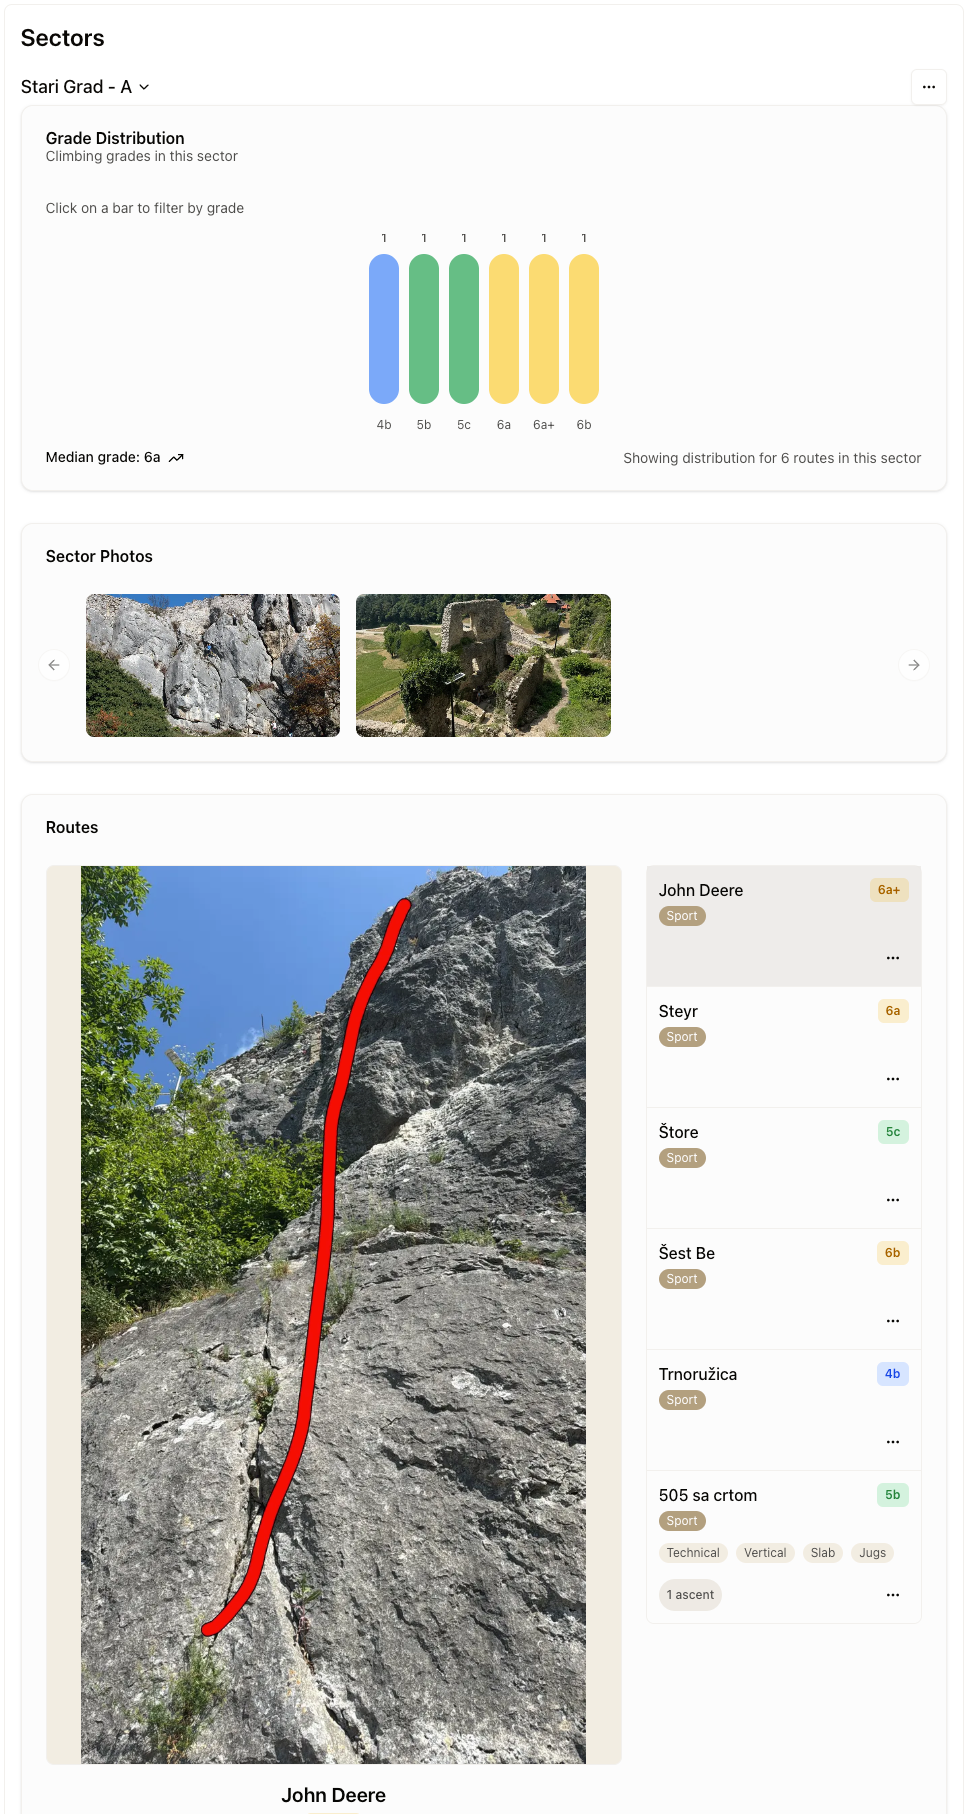
\includegraphics[width=1\textwidth]{images/implementacija/web/crag-details/crag-selected-sector.png}
        \caption{Web aplikacija}
        \label{fig:prikaz_detalja_za_odabrani_sektor_web}
    \end{subfigure}
    \caption{Prikaz detalja za odabrani sektor}
    \label{fig:prikaz_detalja_za_odabrani_sektor}
\end{figure}

Odabirom određenog sektora, korisniku se prikazuje graf težina filtriran po odabranom sektoru, slike sektora te popis svih penjačkih smjerova u tom sektoru. Klikom na određeni stupac na grafu težina, popis penjačkih smjerova se filtrira po označenoj težini. Tablični prikaz je isto dostupan klikom na gumb pored naslova "Sektori" (eng. \textit{Sectors}). Na web aplikaciji nalaze se ista funkcionalnost, ali s različitim prikazom.




\section{Detalji penjačkog smjera}
\section{Prepoznavanje penjačkih smjerova}

TODO: Nedostaju slike

Središnja funkcionalnost aplikacije i prednost u odnosu na postojeća rješenja jest funkcionalnost prepoznavanja i vizualizacije penjačkih smjerova u stvarnom vremenu. Ova mogućnost je dostupna samo u sklopu mobilne aplikacije i direkno rješava problem interpretacije 2D \textit{topo} slika. Pristup ovoj funkcionalnosti omogućen je sa zaslona s detaljnim pregledom penjačkog smjera. Odabirom opcije za prepozavanje, aplikacija aktivira kameru uređaja i pokreće proces temeljen na algoritmima rečunalnog vida. Korisnik usmjerava kameru prema stijeni, a aplikacija u pozadini kontinuirano analizira dobivene slike. Kada je prepoznat penjački smjer korisnik na svom ekranu vidi stvarni svijet s virtualnom linijom koja je nacrtana na stijeni označavajući točnu liniju penjačkog smjera.

Aplikacija nudi korisniku postavke za prilagodbu procesa prepozavanja. Korisnik može birati između dva glavna načina rada. U automatskom načinu rada (eng. \textit{Automatic mode}), aplikacija kontinuirano analizira slike dobivene s kamere i automatski pokušava prepoznati smjer što pruži iskustvo proširene stvarnosti. 

S obzirom na računalno intezivnu prirodu tog procesa, kao alternativu kako bi se smanjila potrošnja resursa, dostupan je i ručni način rada (eng. \textit{Manual mode}). U tom načinu rada, aplikacija ne analizira slike u realnom vremenu, već korisnik samostalno snima fotografiju stijene, a proces prepoznavanja se izvršava samo na toj jednoj, statičnoj slici. 

Dodatno, korisniku su na raspolaganju dostupne i tri razine jačine prepozavanja: \textit{Low}, \textit{Medium} i \textit{High}. Ove postavke u pozadini prilagođavaju parametre algoritama kako bi se postigao kompromis između brzine i kvalitete prepoznavanja. Viša razina jačine prepoznavanja rezultira u preciznijim prepoznavanjima, ali uz veće računsko opterećenje, dok niža nudi brži rad i manju potrošnju. Ove opcije omogućuju korisniku da prilagodi proces prepozavanja prema svojim potrebama i uvjetima.
\section{Korisnički profil}

Svaki registrirani korisnik unutar aplikacije ima pregled profila koji služi kao centralno mjesto za pregled svih njegovih penjačkih aktivnosti i analizu napretka. Pristupom profilu korisniku se prikazuje sažetak njegovih penjačkih aktivnosti poput ukupnog broja posjećenih penjališta, ukupan broj zabilježenih uspona te broj dodanih fotografija.

\begin{figure}[H]
    \centering
    \begin{subfigure}[b]{0.3\textwidth}
        \centering
        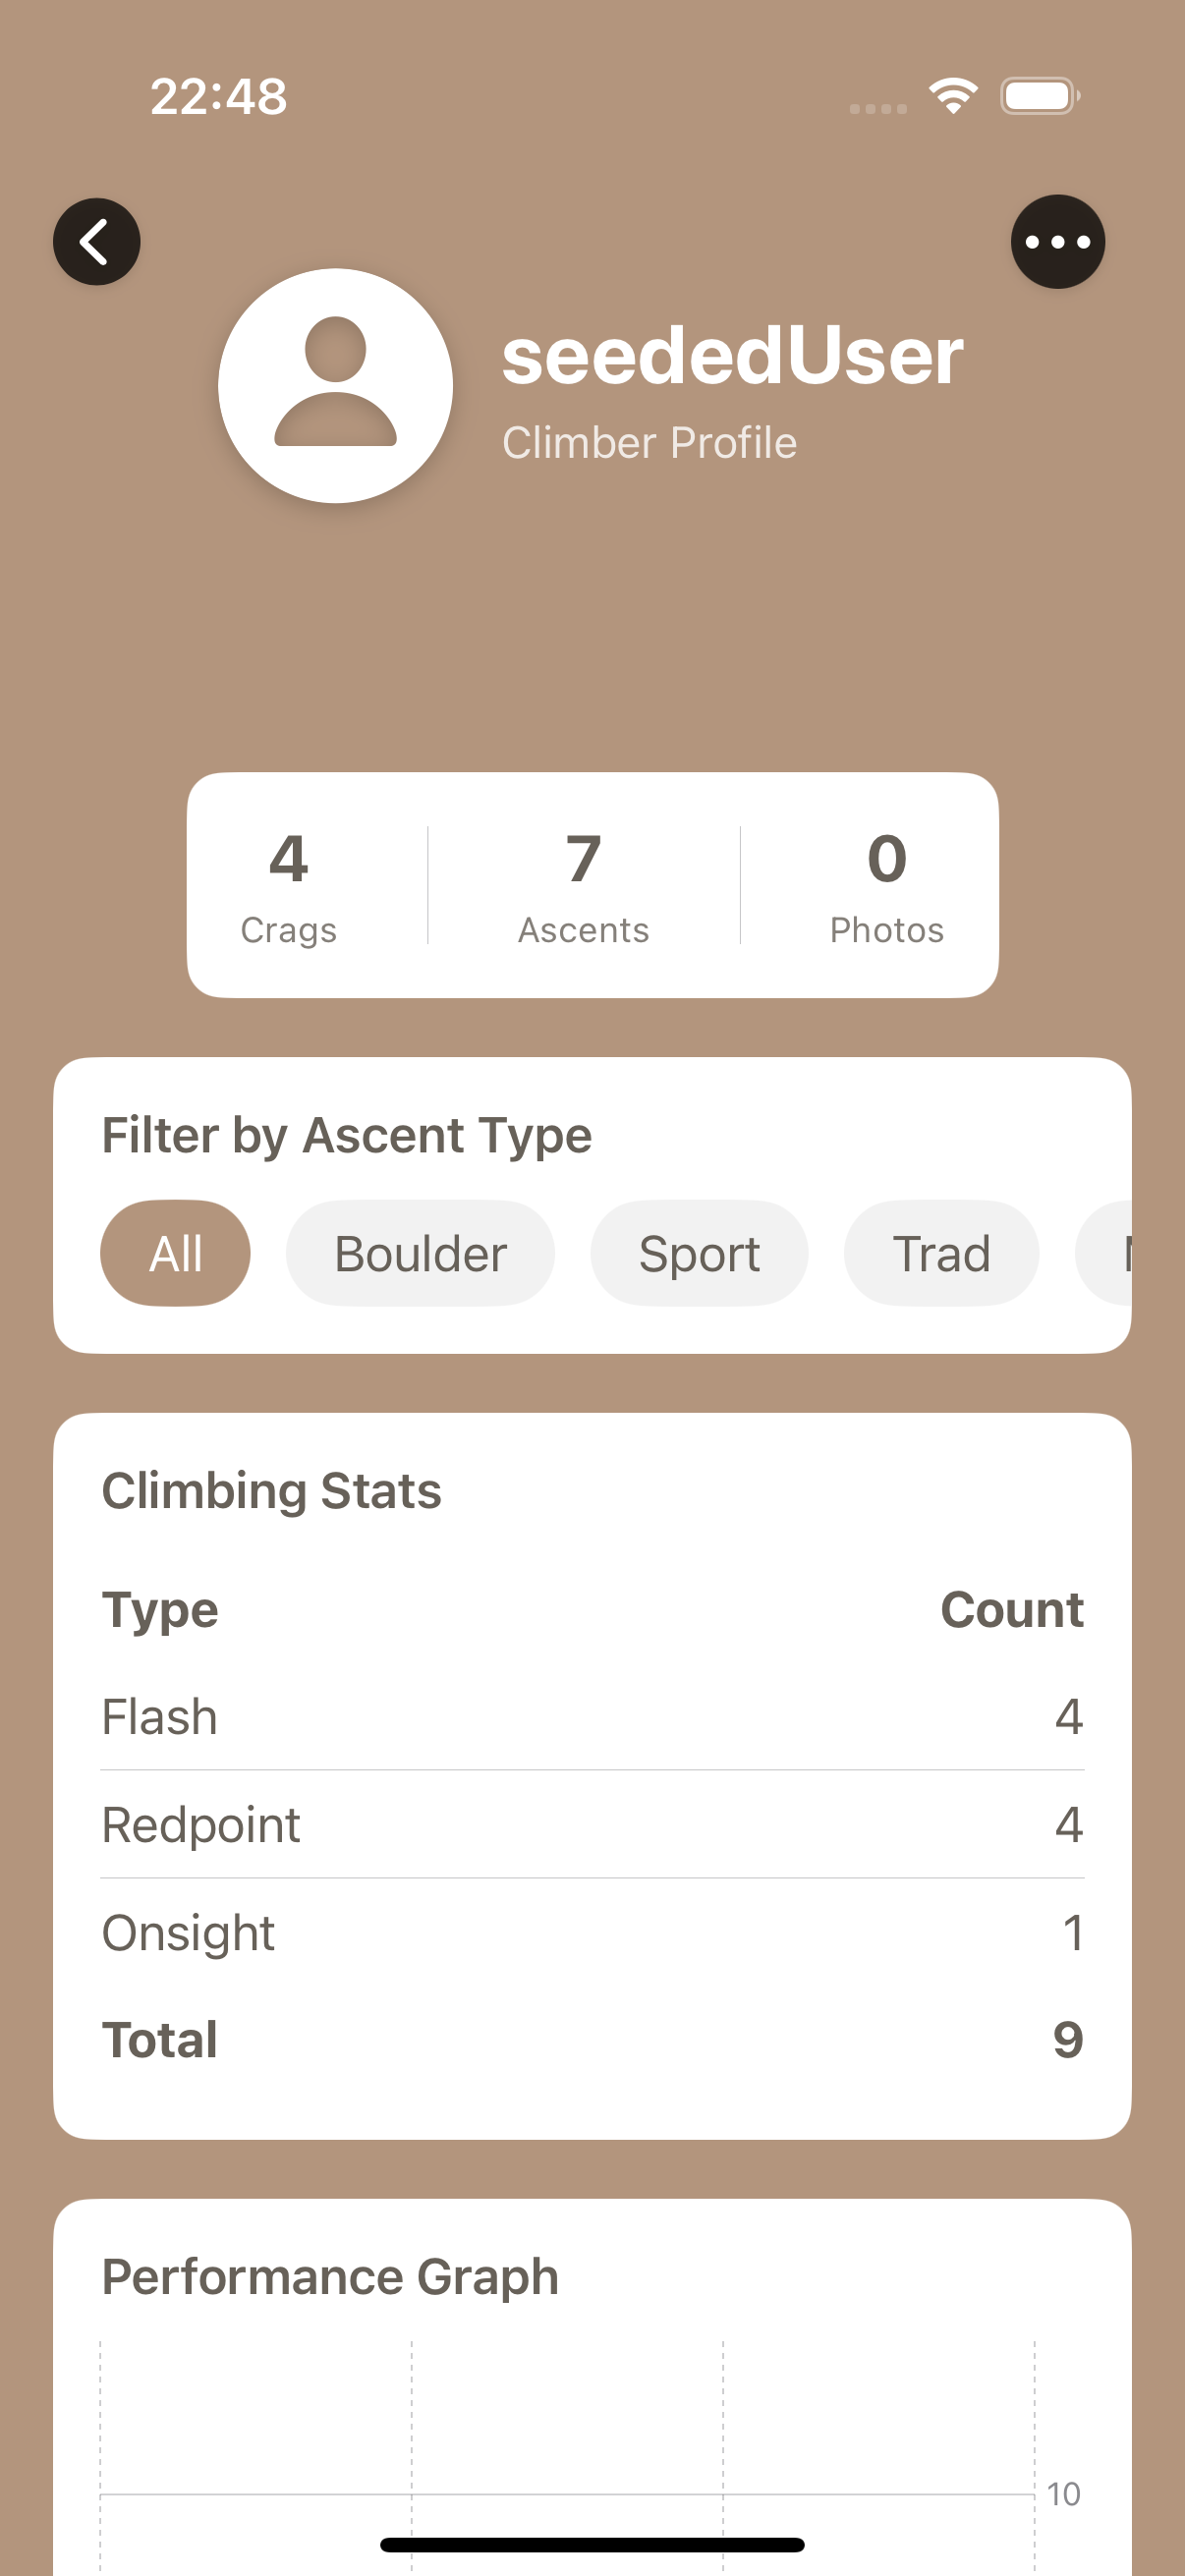
\includegraphics[width=\textwidth]{images/implementacija/user_profile_1.png}
        \caption{Mobilna aplikacija}
        \label{fig:korisnicki_profil_mob}
    \end{subfigure}
    \hfill
    \begin{subfigure}[b]{0.65\textwidth}
        \centering
        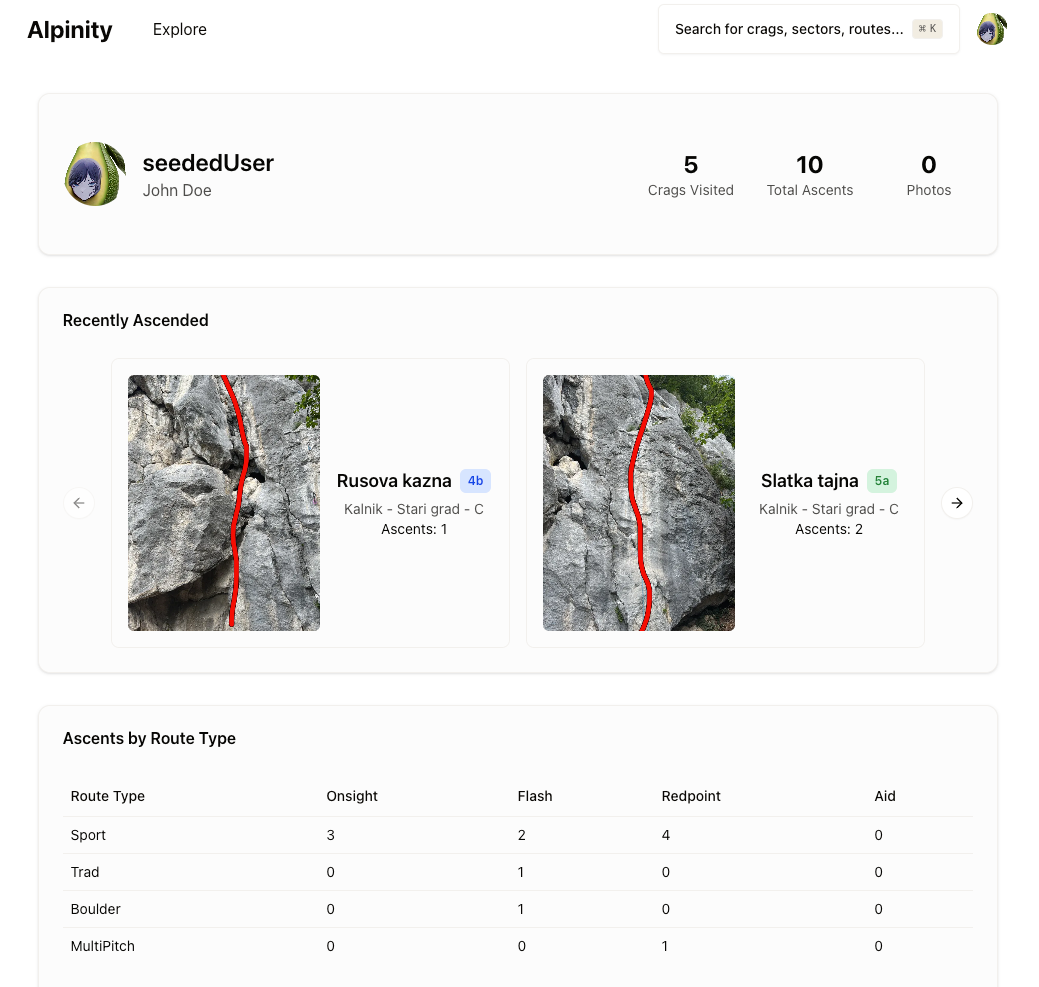
\includegraphics[width=\textwidth]{images/implementacija/web/user-profile-1.png}
        \caption{Web aplikacija}
        \label{fig:korisnicki_profil_web}
    \end{subfigure}
    \caption{Korisnički profil}
    \label{fig:korisnicki_profil}
\end{figure}

Središnji dio profila posvećen je detaljnoj statističkoj analizi (slika~\ref{fig:korisnicki_profil}). Korisnik može filtrirati svoje uspone prema penjačkoj disciplini, poput boulder, sportsko penjanje ili tradicionalno penjanje, kako bi dobio precizniji uvid u svoje aktivnosti. Aplikacija pruža tablični prikaz broja uspona po stilu (Flash, Redpoint, Onsight), omogućujući korisniku da lako vidi koje stilove najčešće prakticira. Dodatno web aplikacija sadrži i nedavno popete penjačke smjerove za korisnika organizirane u horizontalnoj listi sortiranim po datumu uspona od najnovije prema najstarijem.

\begin{figure}[H]
    \centering
    \begin{subfigure}[b]{0.3\textwidth}
        \centering
        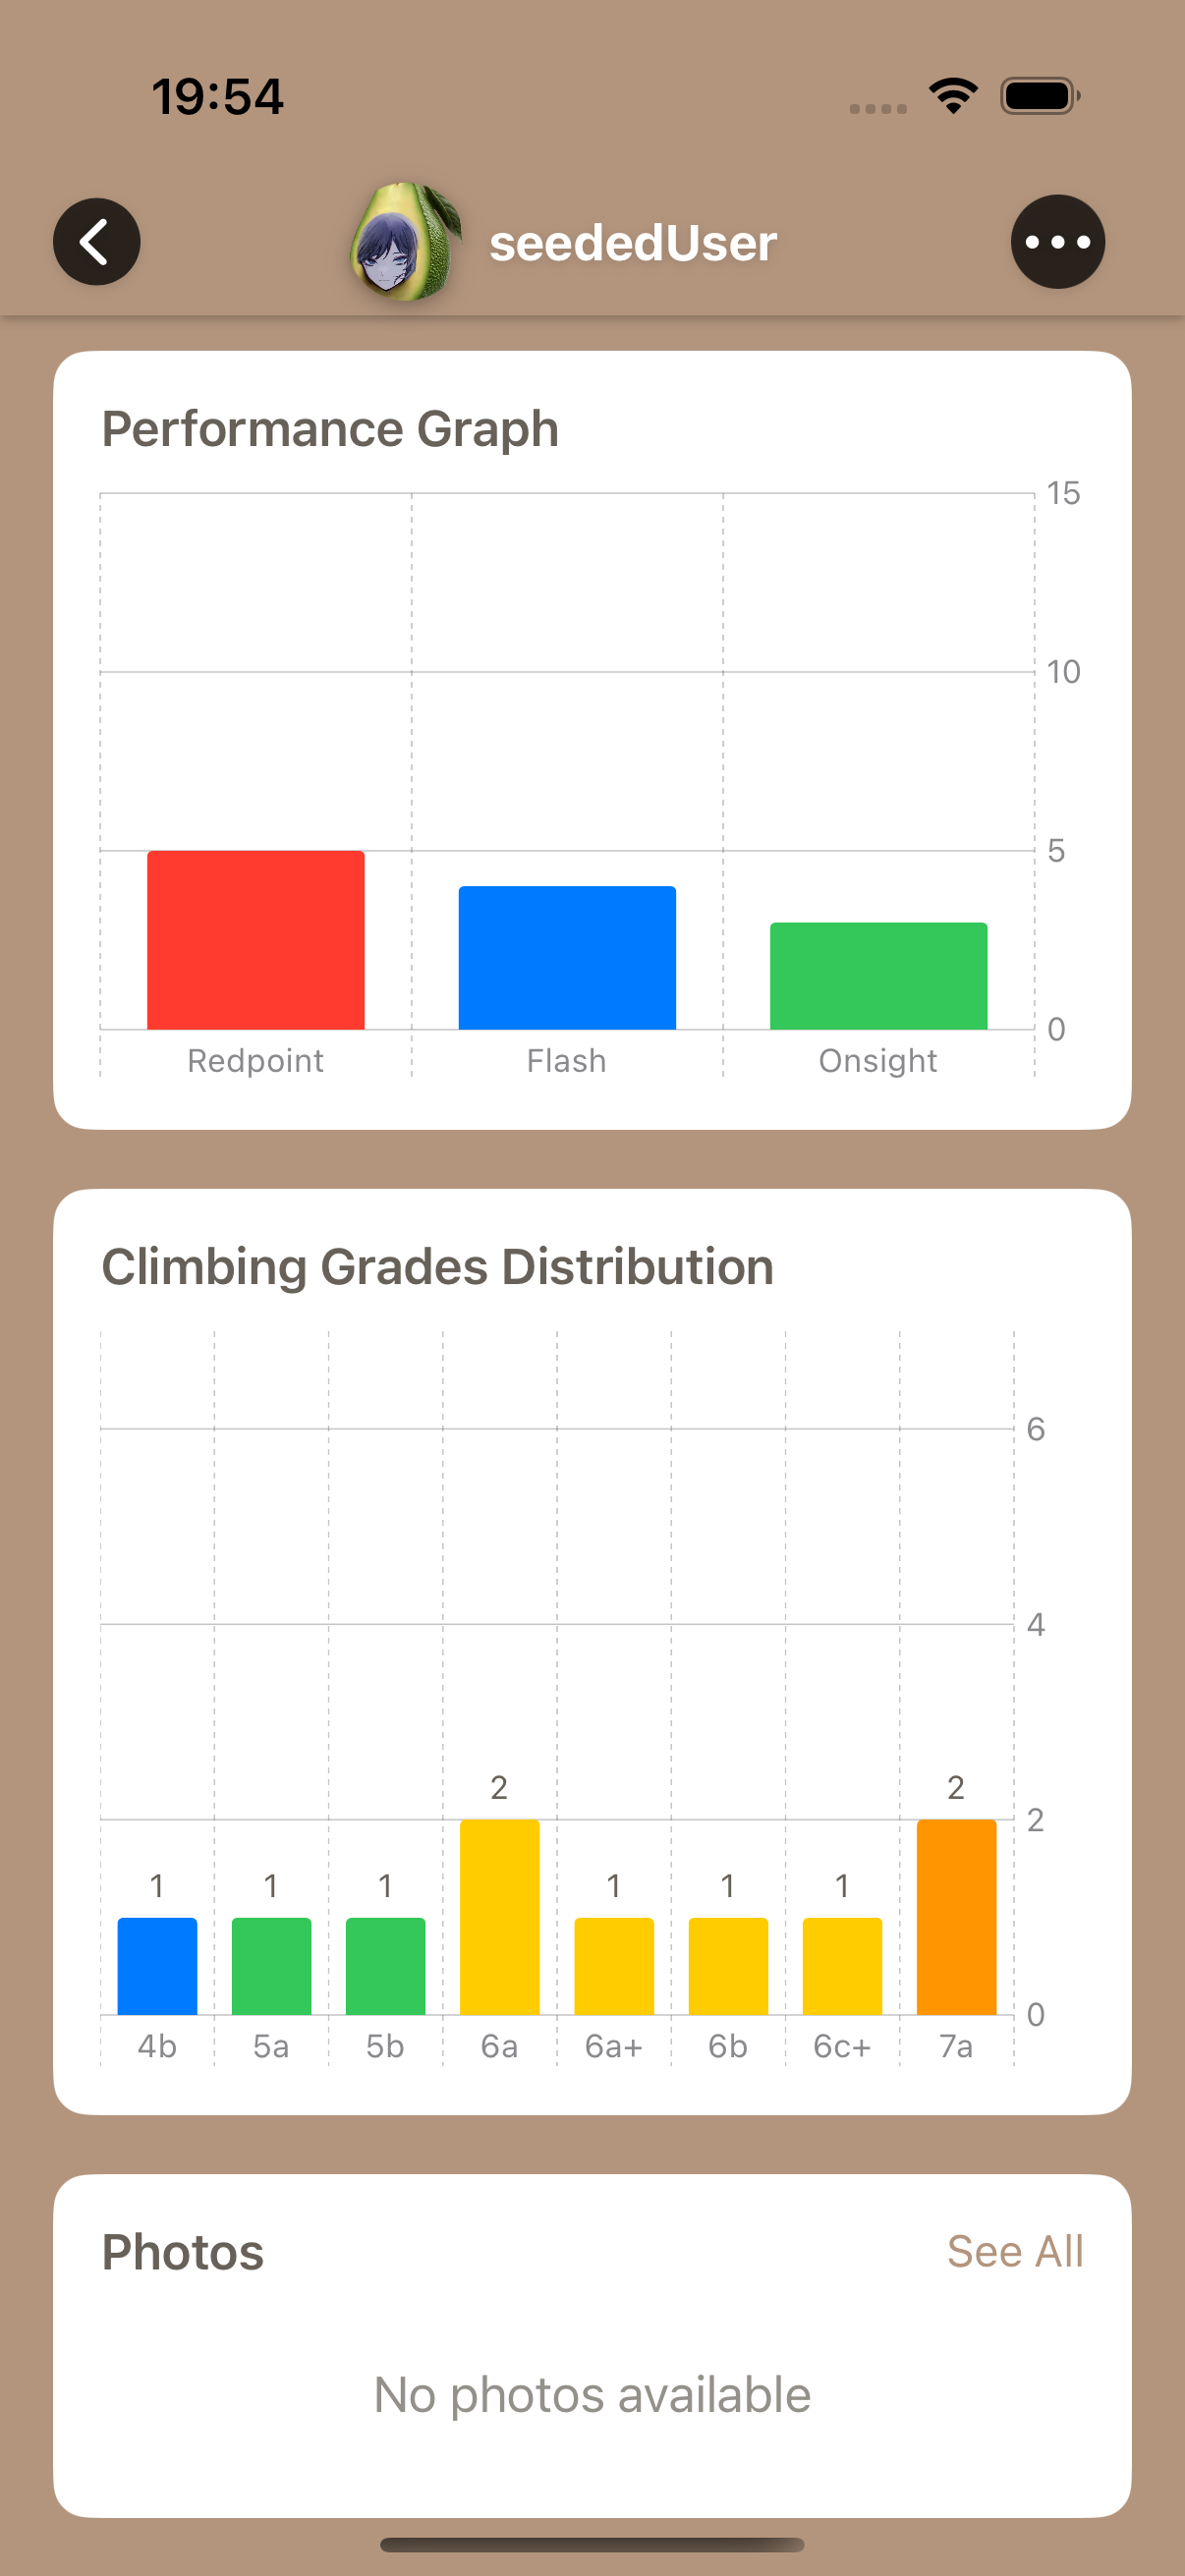
\includegraphics[width=\textwidth]{images/implementacija/user_profile_2.png}
        \caption{Mobilna aplikacija}
        \label{fig:korisnicki_profil_graf_mob}
    \end{subfigure}
    \hfill
    \begin{subfigure}[b]{0.65\textwidth}
        \centering
        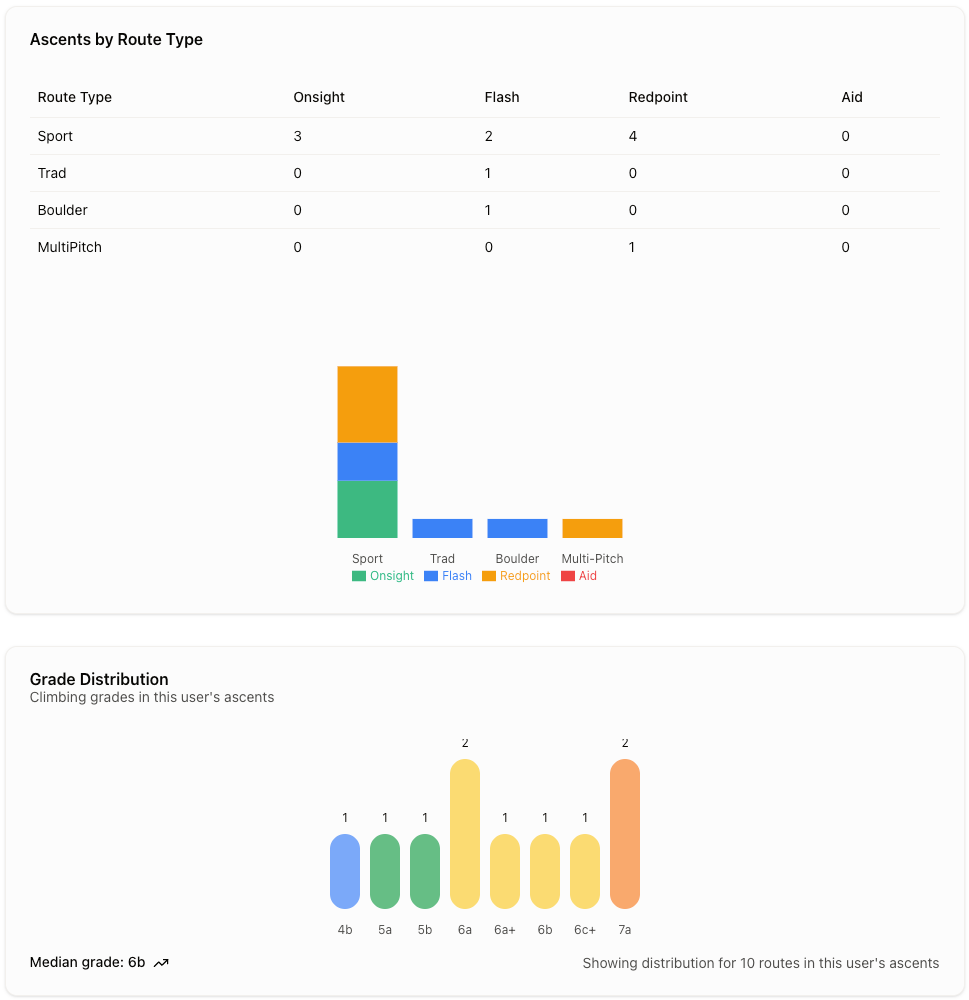
\includegraphics[width=\textwidth]{images/implementacija/web/user-profile-2.png}
        \caption{Web aplikacija}
        \label{fig:korisnicki_profil_graf_web}
    \end{subfigure}
    \caption{Grafovi performansi i distribucije po ocjenama}
    \label{fig:korisnicki_profil_2}
\end{figure}

Za bolju vizualizaciju, podaci su prikazani i u dva ključna grafa (slika~\ref{fig:korisnicki_profil_2}). Graf performansi prikazuje distribuciju uspona po stilu, dok graf distribucije po ocjenama prikazuje stupčastim diagramom, odnosno koliko je penjačkih smjerova određene težine je korisnik uspješno popeo. Ovi grafički prikazi omogućuju procjenu vlastitih sposobnosti i napretka tokom vremena. Finalno na dnu profila nalazi se i lista svih slika kojima korisnik želi istaknuti svoj profil.

\begin{figure}[H]
    \centering
    \begin{subfigure}[b]{0.33\textwidth}
        \centering
        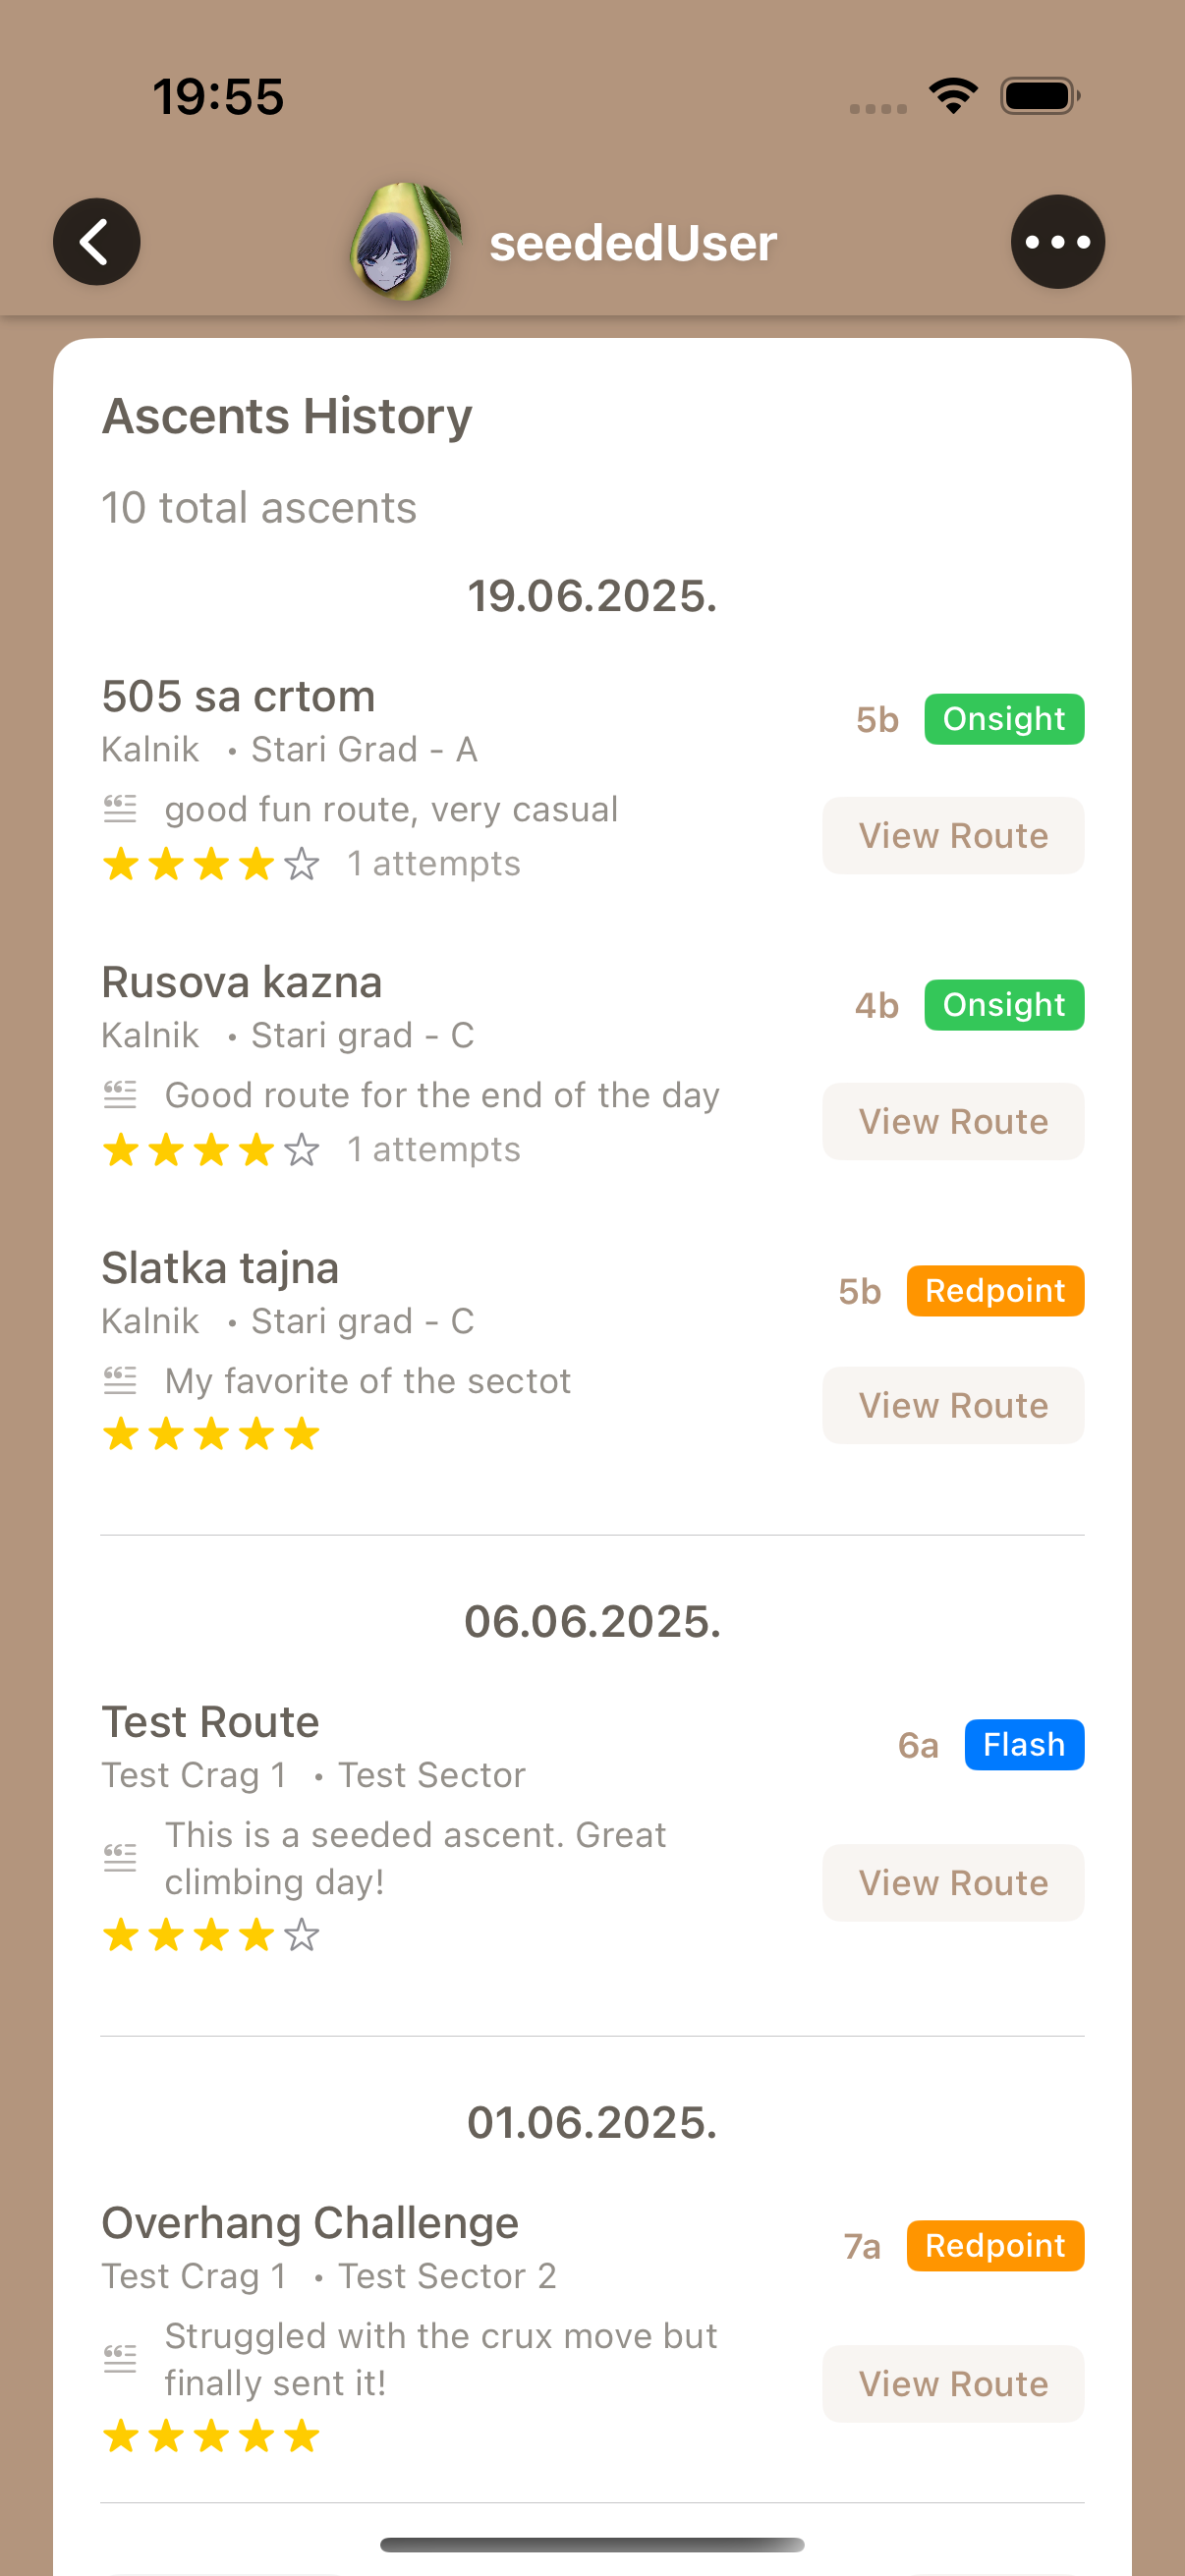
\includegraphics[width=\textwidth]{images/implementacija/user_profile_3.png}
        \caption{Mobilna aplikacija}
        \label{fig:korisnicki_profil_povijest_mob}
    \end{subfigure}
    \hfill
    \begin{subfigure}[b]{0.65\textwidth}
        \centering
        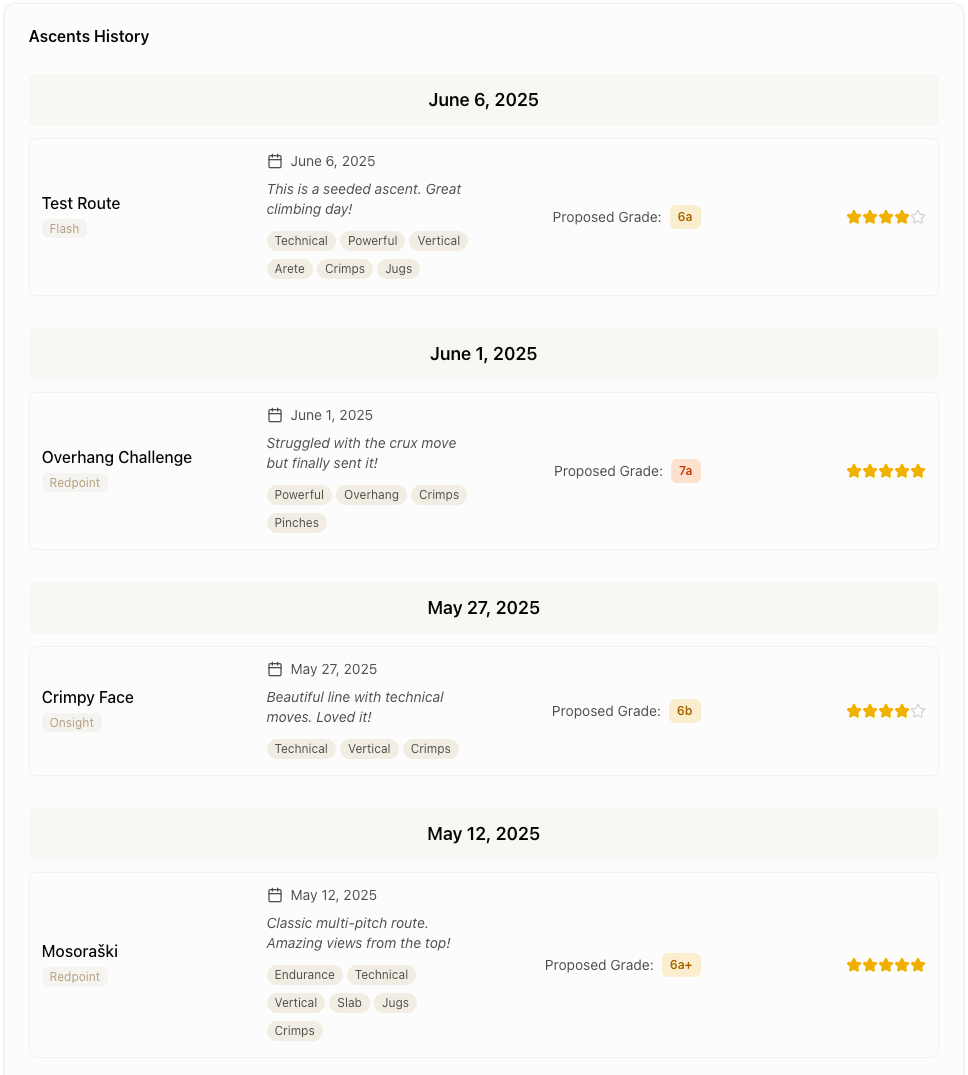
\includegraphics[width=\textwidth]{images/implementacija/web/user-profile-3.png}
        \caption{Web aplikacija}
        \label{fig:korisnicki_profil_povijest_web}
    \end{subfigure}
    \caption{Povijest uspona}
    \label{fig:korisnički_profil_3}
\end{figure}

Osim statistike, profil sadrži i povijest svih uspona, kronološki poredanih od najnovijeg prema najstarijem (slika~\ref{fig:korisnički_profil_3}). Svaki unos u povijest sadrži sve relevantne informacije poput datuma, naziva penjačkog smjera, lokaciju, težinu, stil uspona, osobni komentar i ocjenu smjera te direktnu poveznicu na detaljni pregled samog penjačkog smjera. Ovaj dnevnik služi kao vrijedan alat za prisjećanje na prethodna penjačka iskustva.

\subsection{Korisnički profil drugog korisnika}

Pretraživanjem korisničkog profila drugog korisnika, korisnik može vidjeti statistike, grafove performansi i povijest uspona drugog korisnika na isti način kao i na vlastitom profilu (slika~\ref{fig:korisnički_profil_other}).


\begin{figure}[H]
    \centering
    \begin{subfigure}[b]{0.33\textwidth}
        \centering
        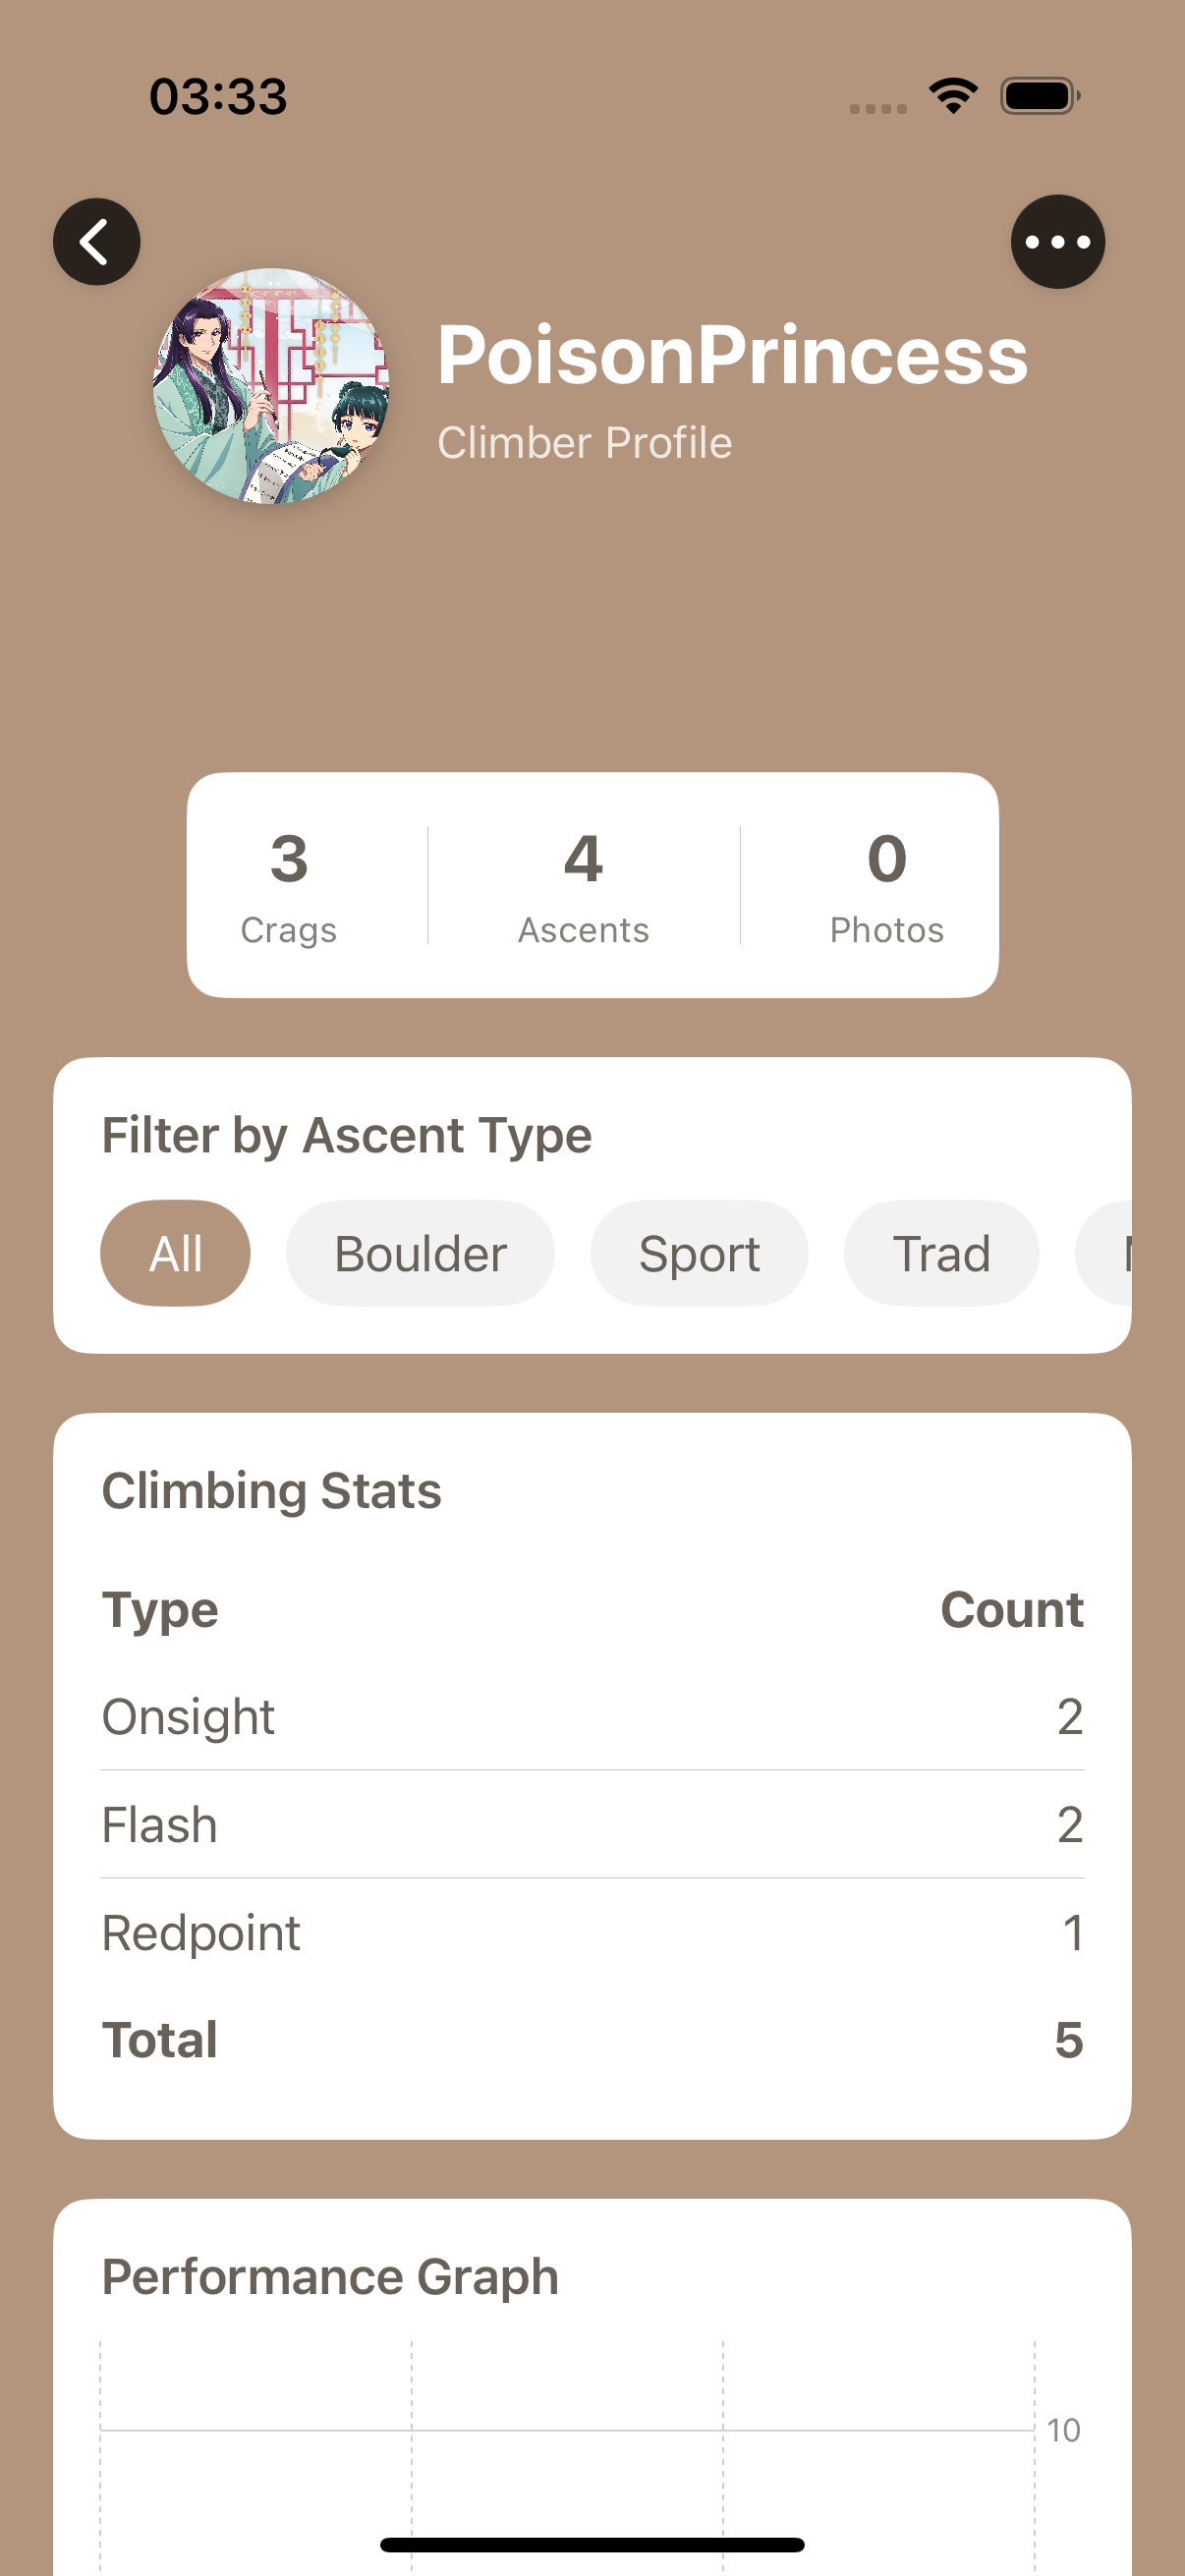
\includegraphics[width=\textwidth]{images/implementacija/user-profile-other.png}
        \caption{Mobilna aplikacija}
        \label{fig:korisnicki_profil_other_mob}
    \end{subfigure}
    \hfill
    \begin{subfigure}[b]{0.65\textwidth}
        \centering
        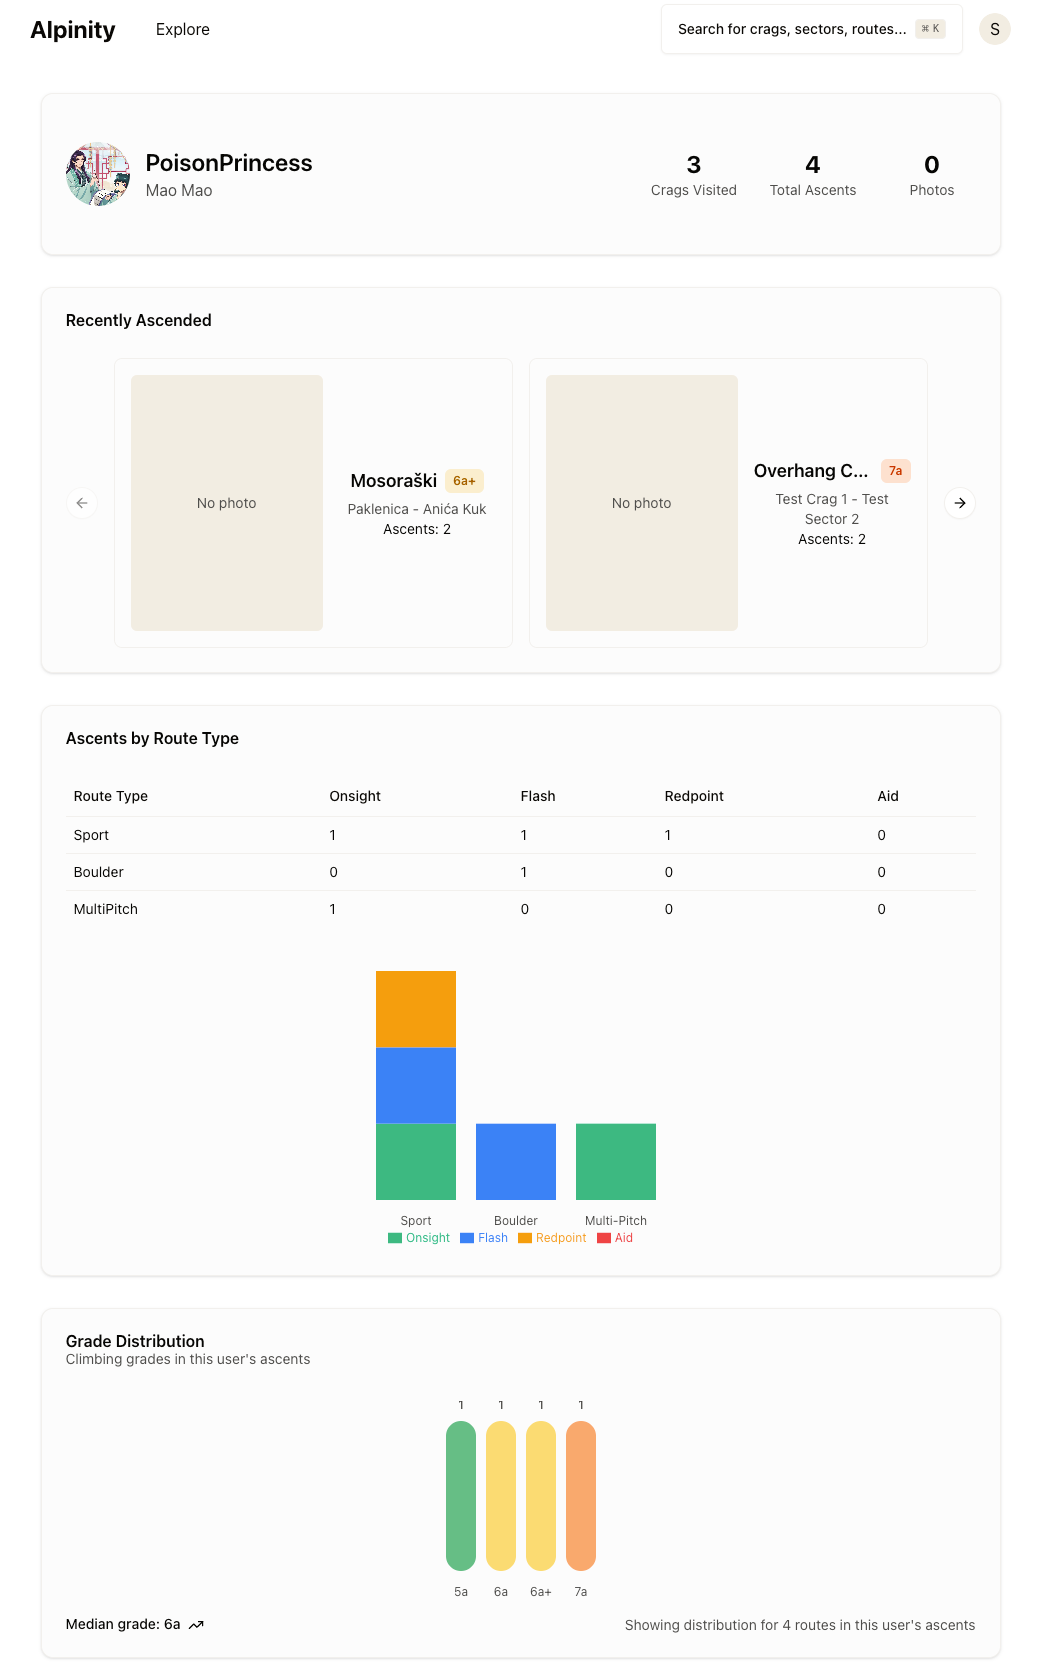
\includegraphics[width=\textwidth]{images/implementacija/web/user-profile-other.png}
        \caption{Web aplikacija}
        \label{fig:korisnicki_profil_other_web}
    \end{subfigure}
    \caption{Korisnički profil drugog korisnika}
    \label{fig:korisnički_profil_other}
\end{figure}

\section{Unos i uređivanje podataka}

Kako bi sustav bio dinamičan i ažuran, aplikacija omogućuje ovlaštenim korisnicima kreiranje i uređivanje svih hijerarhijskih razina podataka, od penjališta do pojedinačnih penjačkih smjerova.

\subsection{Dodavanje, uređivanje i brisanje penjališta}

Na korisničkom profilu omogućeno je kreiranje novog penjališta u izborniku u gornjem desnom kutu korisničkog profila. Na web aplikaciji ta opcija se nalazi u navigacijskoj traci u postavkama korisničkog izbornika. Funkcionalnost kreiranja novog penjališta nije dostupna svim korisnicima, već je ograničena na one s posebnim ovlastima, a to su administratori sustava i verificirani korisnici (eng. \textit{creators}). 

\begin{figure}[H]
    \centering
    \begin{subfigure}[b]{0.31\textwidth}
        \centering
        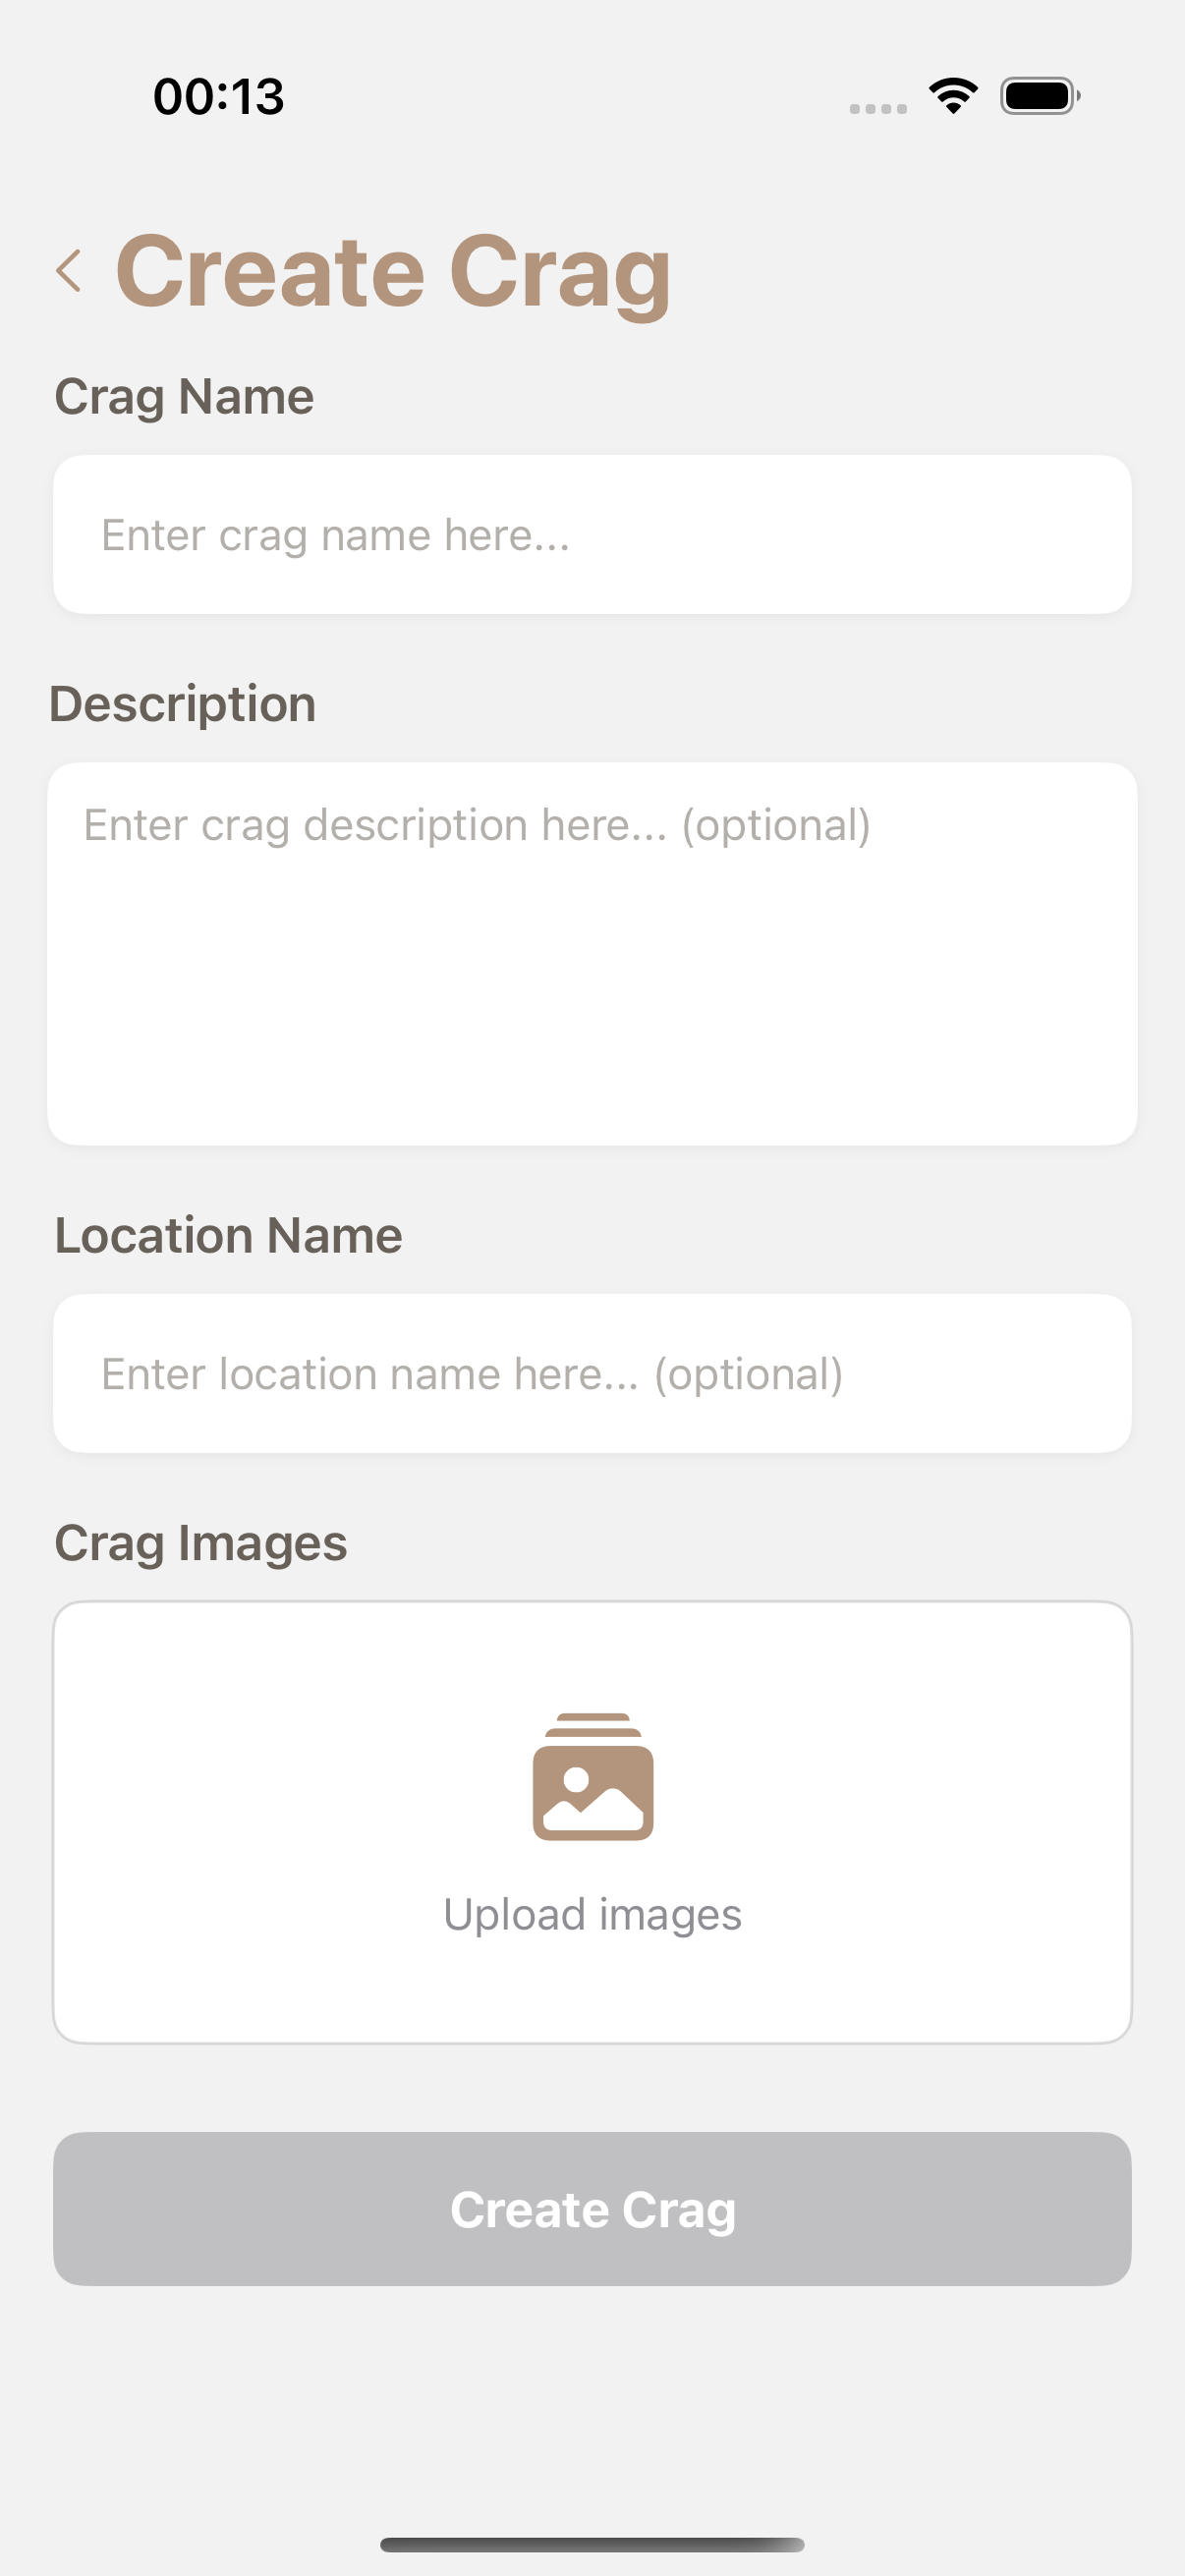
\includegraphics[width=\textwidth]{images/implementacija/editing-options/create_crag.png}
        \caption{Mobilna aplikacija}
        \label{fig:dodavanje_lokacije_mob}
    \end{subfigure}
    \hfill
    \begin{subfigure}[b]{0.6\textwidth}
        \centering
        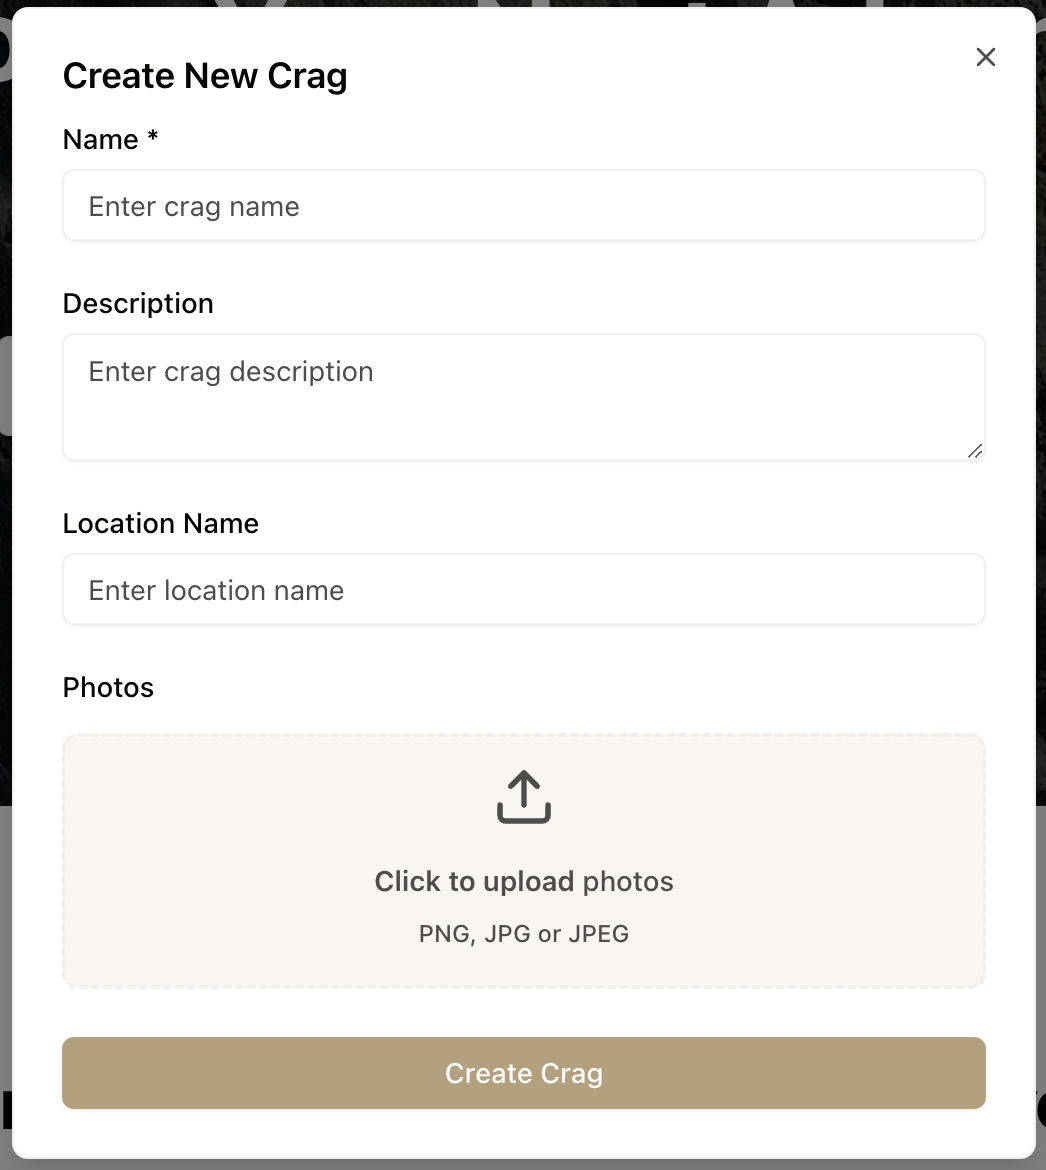
\includegraphics[width=\textwidth]{images/implementacija/web/editing-options/create-crag.png}
        \caption{Web aplikacija}
        \label{fig:dodavanje_lokacije_web}
    \end{subfigure}
    \caption{Dodavanje novog penjališta}
    \label{fig:dodavanje_lokacije}
\end{figure}

Ovlašteni korisnik odabirom ove opcije pristupa formi za unos novog (slika~\ref{fig:dodavanje_lokacije}). Potrebno je unijeti naziv penjališta, opcionalni opis koji može sadržavati informacije o povijesti regije ili slične zanimljivosti, te naziv šire geografske lokacije. Ime geografske lokacije korisnik može samostalno dodati, no ako ne postoji, aplikacija će automatski dodati naziv geografske lokacije na temelju lokacije penjališta. Ključno, korisnik može dodati jednu ili više fotografija koje vizualno predstavljaju penjalište. Nakon unosa svih podataka, novo penjalište se stvara u sustavu i postaje dostupna svim korisnicima.

\begin{figure}[H]
    \centering
    \begin{subfigure}[b]{0.36\textwidth}
        \centering
        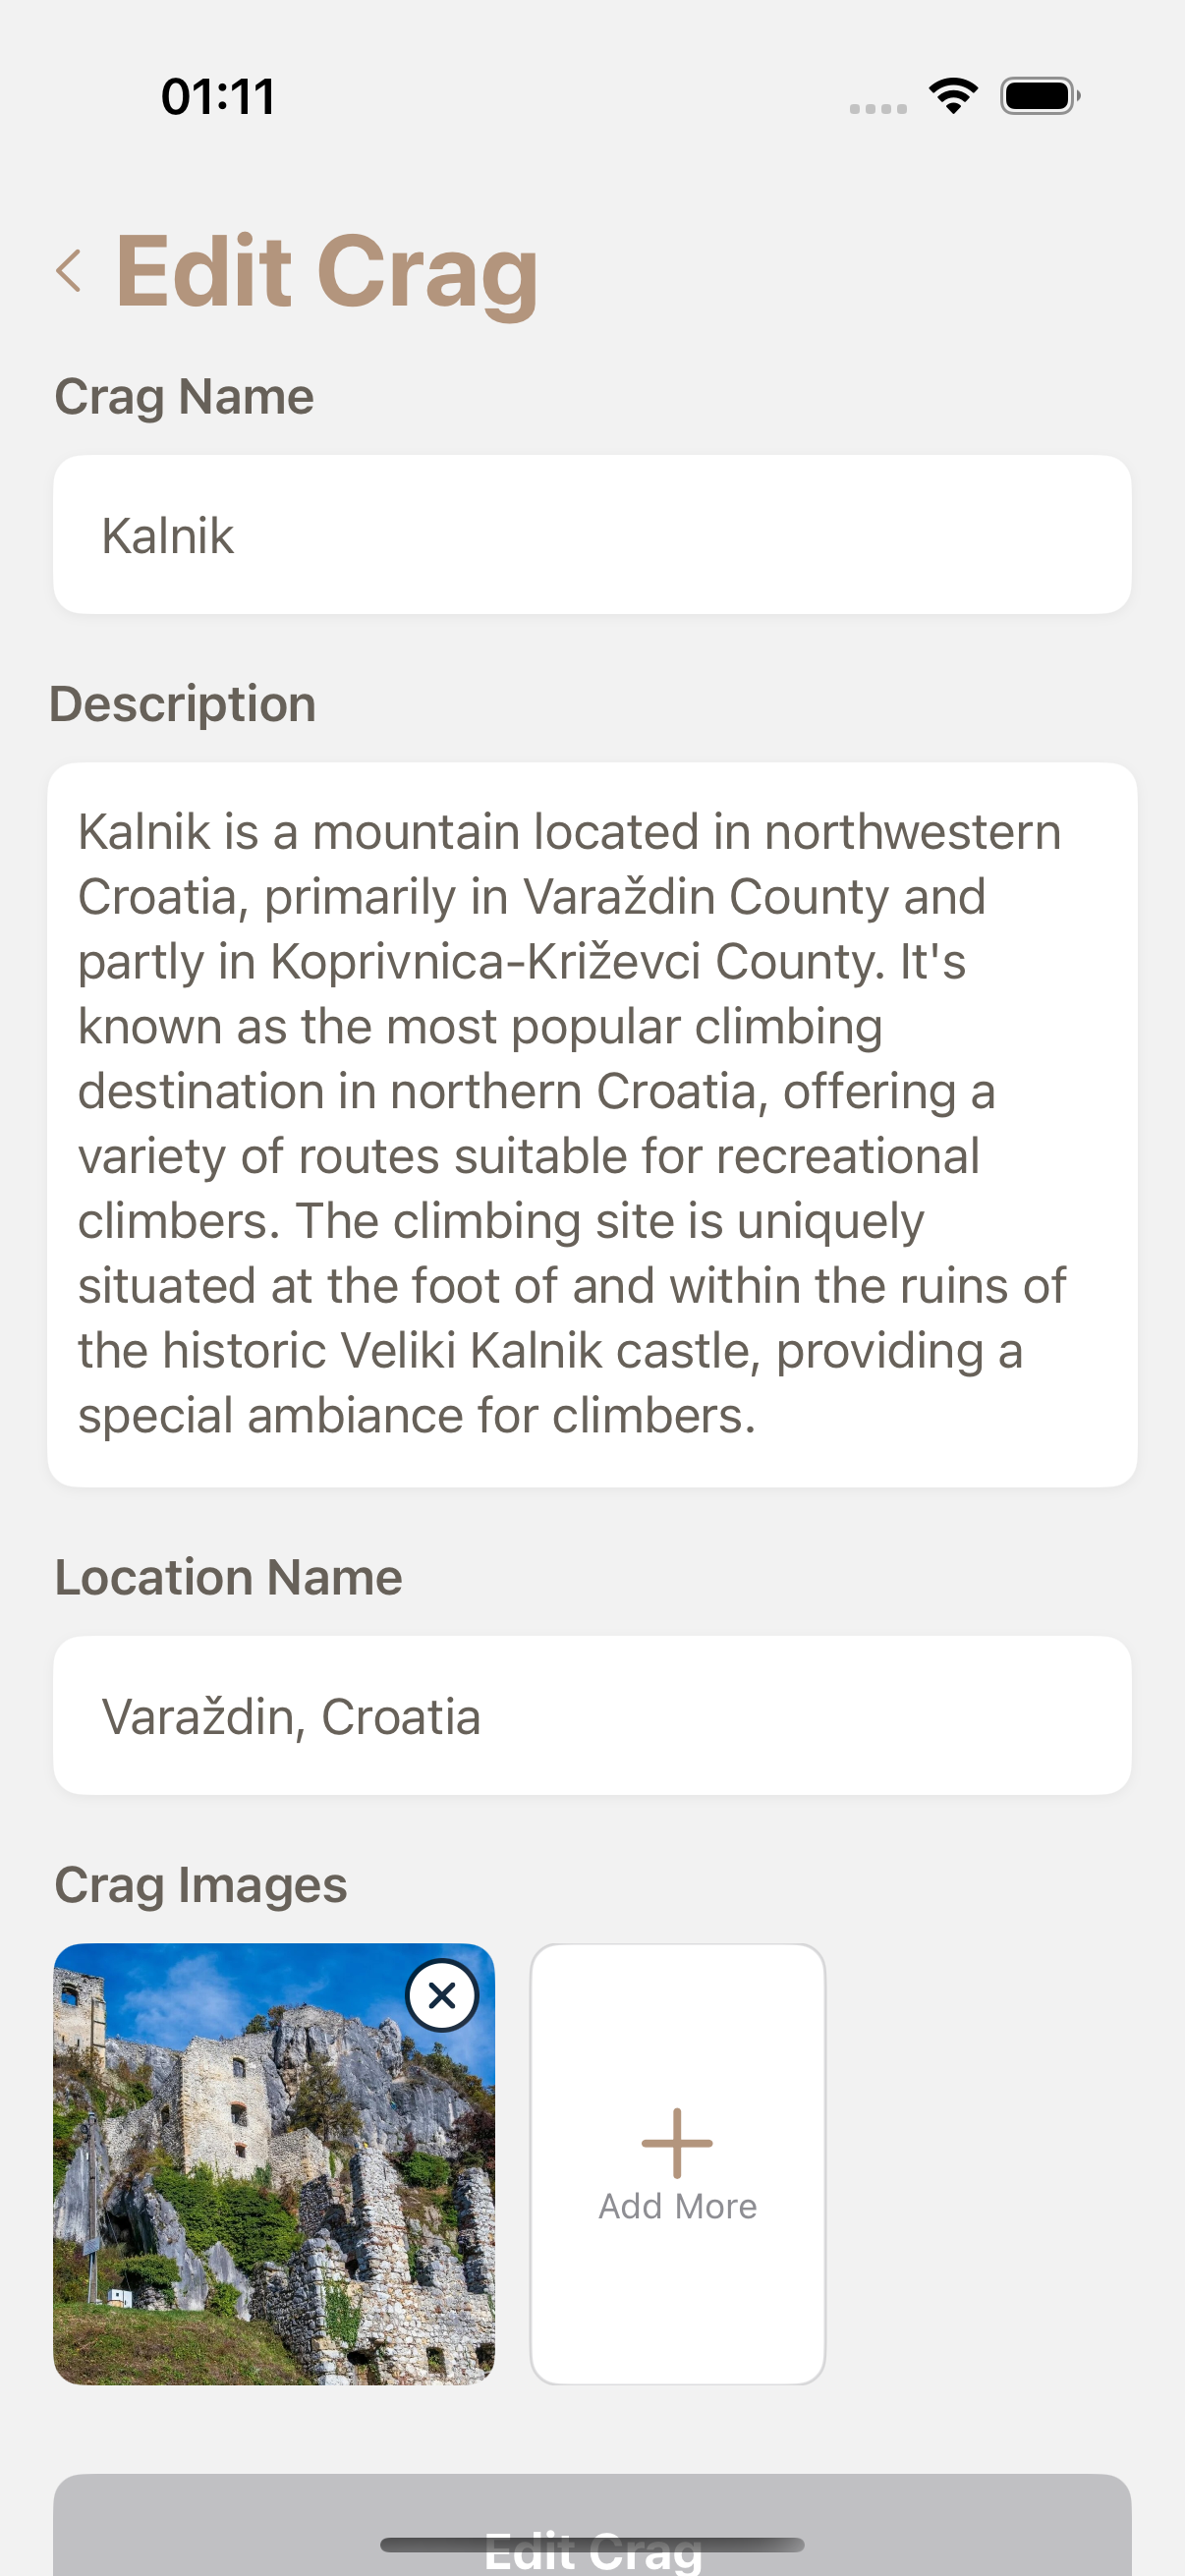
\includegraphics[width=\textwidth]{images/implementacija/editing-options/edit-crag.png}
        \caption{Mobilna aplikacija}
        \label{fig:uredjivanje_lokacije_mob}
    \end{subfigure}
    \hfill
    \begin{subfigure}[b]{0.47\textwidth}
        \centering
        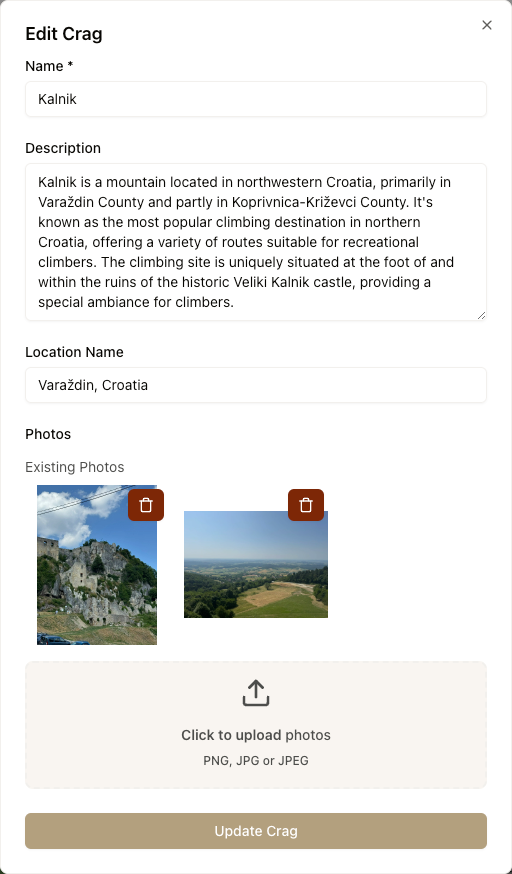
\includegraphics[width=\textwidth]{images/implementacija/web/editing-options/edit-crag.png}
        \caption{Web aplikacija}
        \label{fig:uredjivanje_lokacije_web}
    \end{subfigure}
    \caption{Uređivanje postojećeg penjališta}
    \label{fig:uredjivanje_lokacije}
\end{figure}

Osim kreiranja novih, ovlašteni korisnici imaju mogućnost i uređivanja postojećih penjališta (slika~\ref{fig:uredjivanje_lokacije}). Pristup ovoj funkcionalnosti omogućen je u izborniku na zaslonu s detaljnim pregledom penjališta. 
Sučelje za uređivanje omogućuje promjenu svih prethodno unesenih podataka, uključujući naziv, opis i naziv geografske lokacije. Korisnici također mogu upravljati galerijom fotografija, dodajući nove ili uklanjajući postojeće slike. 

Brisanje penjališta dostupno je u izborniku na zaslonu detaljnog pregleda penjališta. Klikom na opciju "Izbriši penjalište" (eng. \textit{Delete crag}) korisniku se prikazuje prozor s upitom o potvrdi brisanja. Ako korisnik potvrdi brisanje, penjalište se briše iz sustava i postaje nedostupno svim korisnicima.

\subsection{Upravljanje korisničkim ovlastima}

Kako bi se osigurala kontrola nad unosom i uređivanjem podataka, a istovremeno omogućio doprinos više ljudi, sustav implementira mehanizam za upravljanje korisničkim ovlastima na razini pojedine penjališta. Ovoj funkcionalnosti imaju pristup samo vlasnik penjališta i administratori sustava putem izbornika na zaslonu s detaljnim pregledom penjališta. 

\begin{figure}[H]
    \centering
    \begin{subfigure}[b]{0.36\textwidth}
        \centering
        
\includegraphics[width=\textwidth]{images/implementacija/editing-options/manage-users.png}
        \caption{Mobilna aplikacija}
        \label{fig:upravljanje_ovlastima_mob}
    \end{subfigure}
    \hfill
    \begin{subfigure}[b]{0.6\textwidth}
        \centering
        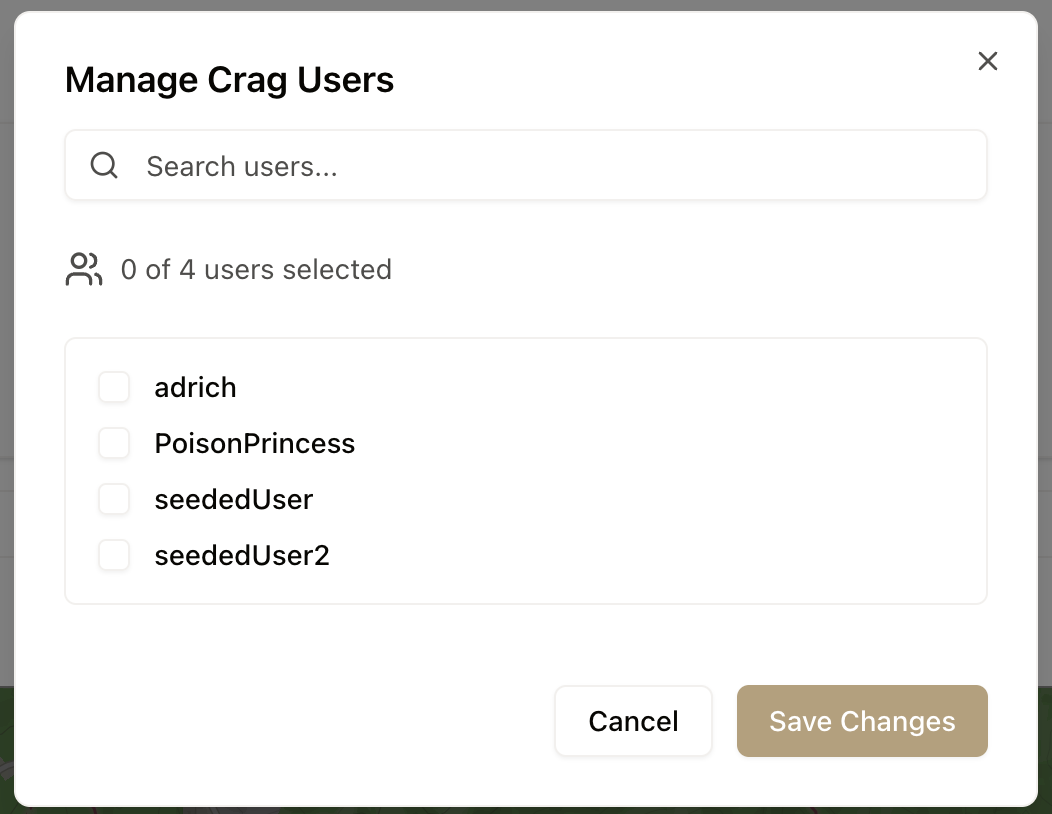
\includegraphics[width=\textwidth]{images/implementacija/web/editing-options/manage-users.png}
        \caption{Web aplikacija}
        \label{fig:upravljanje_ovlastima_web}
    \end{subfigure}
    \caption{Upravljanje korisničkim ovlastima}
    \label{fig:upravljanje_ovlastima}
\end{figure}

Pristupom pregledu za upravljanje ovlastima prikazuje se popis svih korisnika koji trenutno imaju ili mogu dobiti dozvole za uređivanje sadržaja na tom penjalištu (slika~\ref{fig:upravljanje_ovlastima}). Sučelje omogućuje pretragu korisnika po korisničkom imenu te odabir jednog ili više korisnika kojima se žele dodijeliti ili oduzeti ovlasti uređivanja. Time odabrani korisnik dobiva prava uređivanja penjališta bez davanja potpunih administrativnih ili kreator prava.


\subsection{Dodavanje, uređivanje i brisanje sektora}

Unutar svakog penjališta, ovlašteni korisnici mogu dalje strukturirati sadržaj kreiranjem i uređivanjem sektora. Pristup opciji za dodavanje nalazi se u izborniku na zaslonu s detaljnim pregledom penjališta. 

\begin{figure}[H]
    \centering
    \begin{subfigure}[b]{0.36\textwidth}
        \centering
        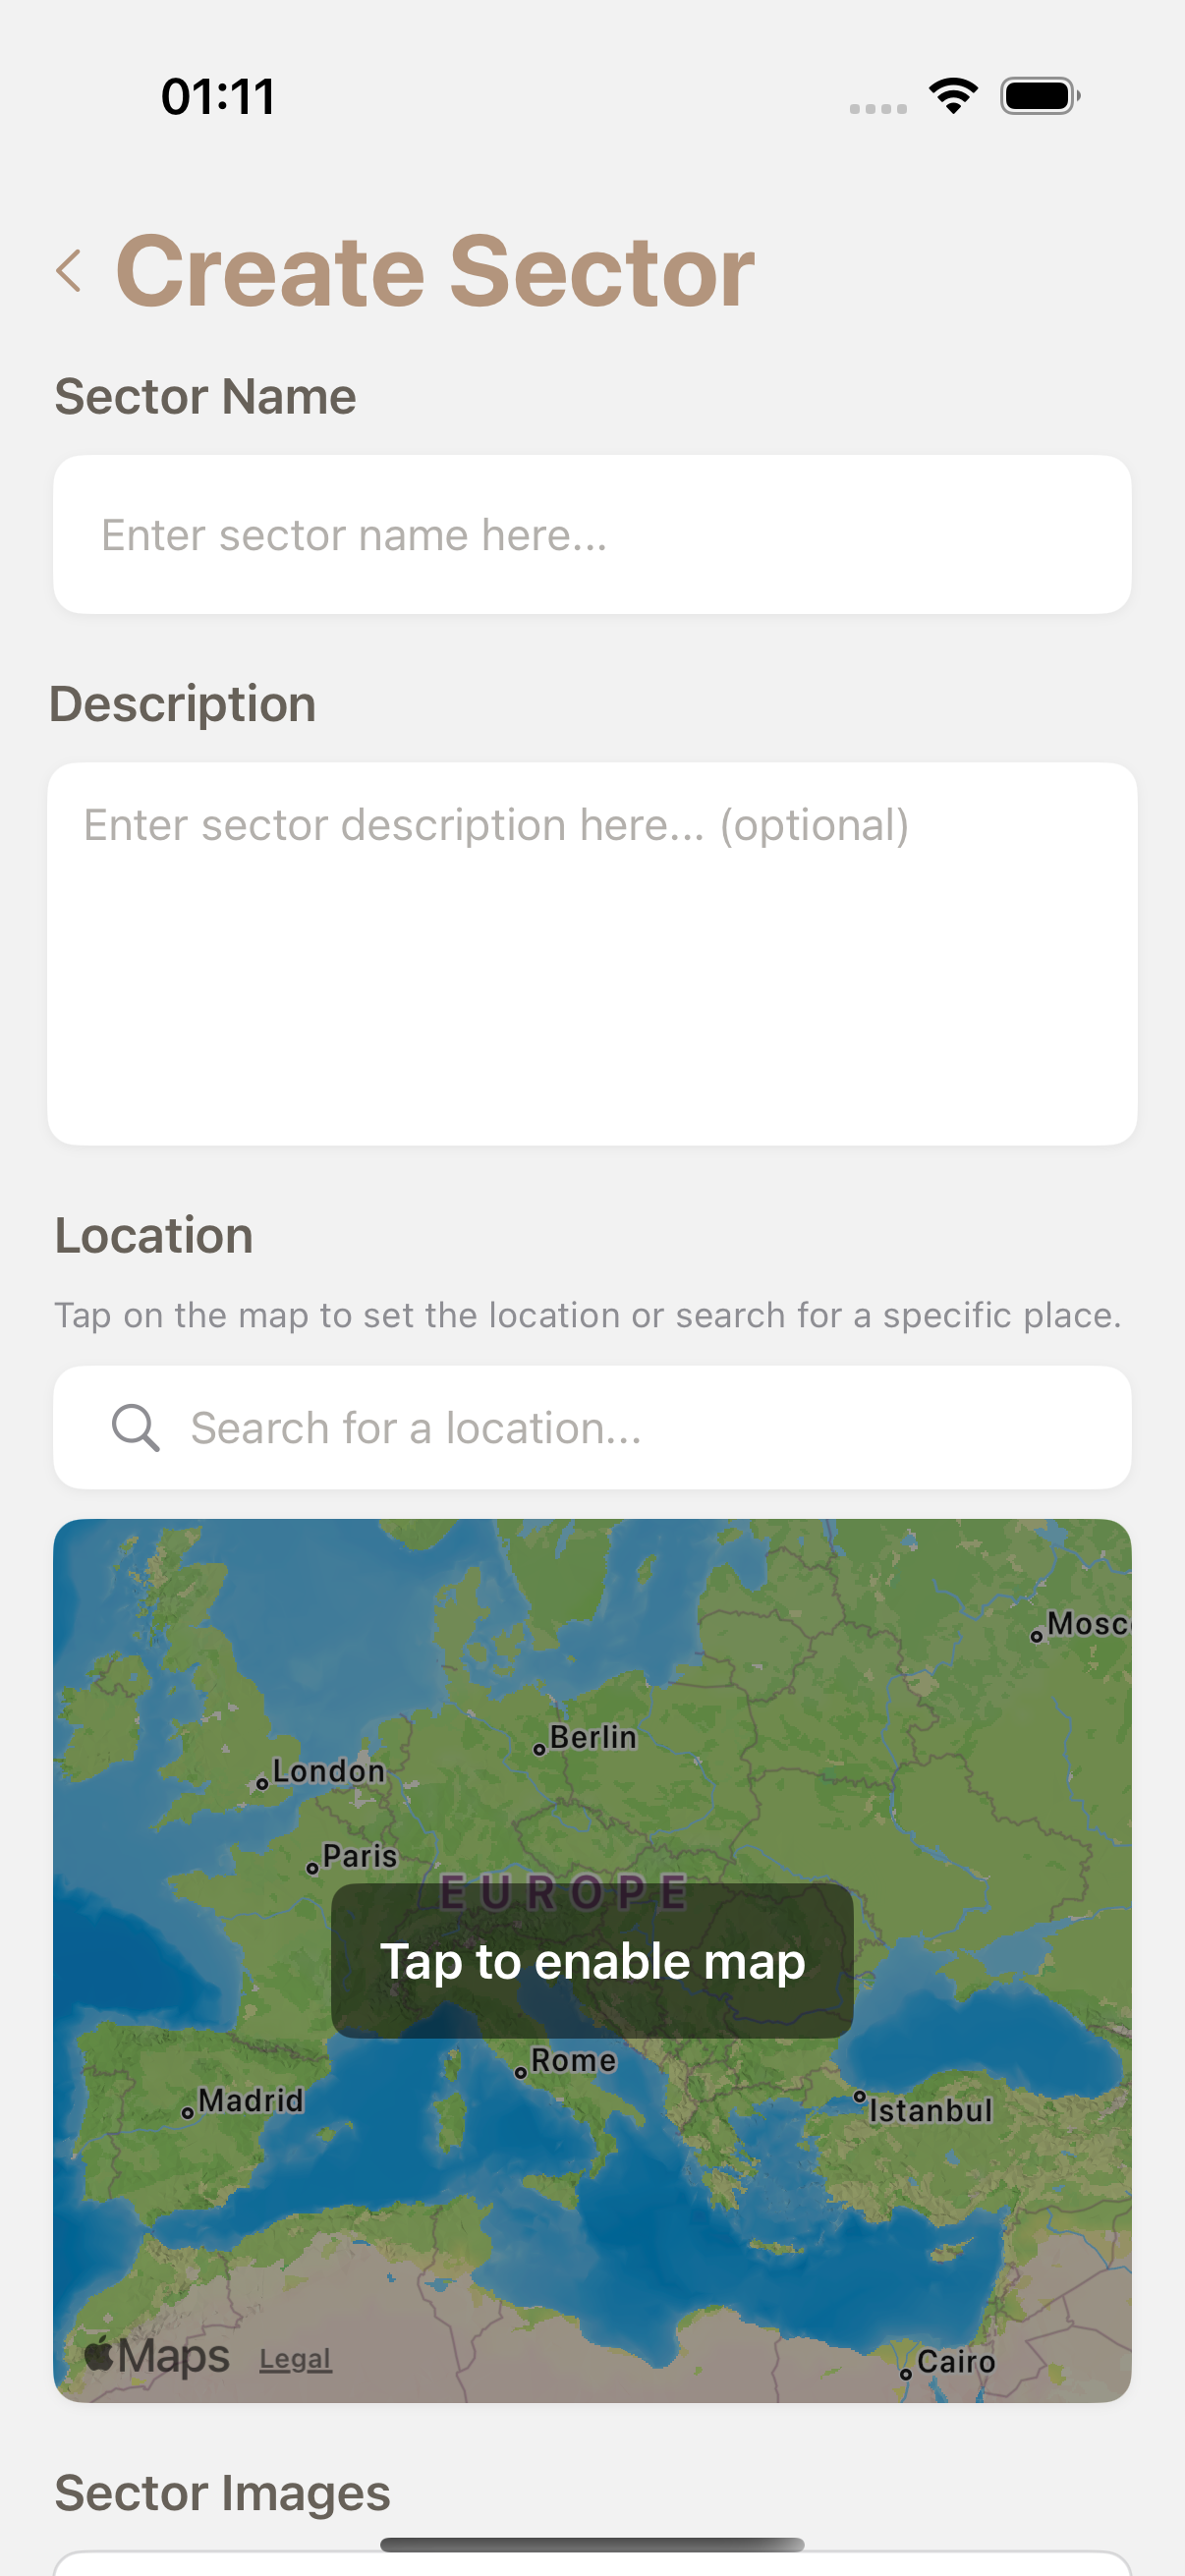
\includegraphics[width=\textwidth]{images/implementacija/editing-options/create-sector.png}
        \caption{Mobilna aplikacija}
        \label{fig:dodavanje_sektora_mob}
    \end{subfigure}
    \hfill
    \begin{subfigure}[b]{0.45\textwidth}
        \centering
        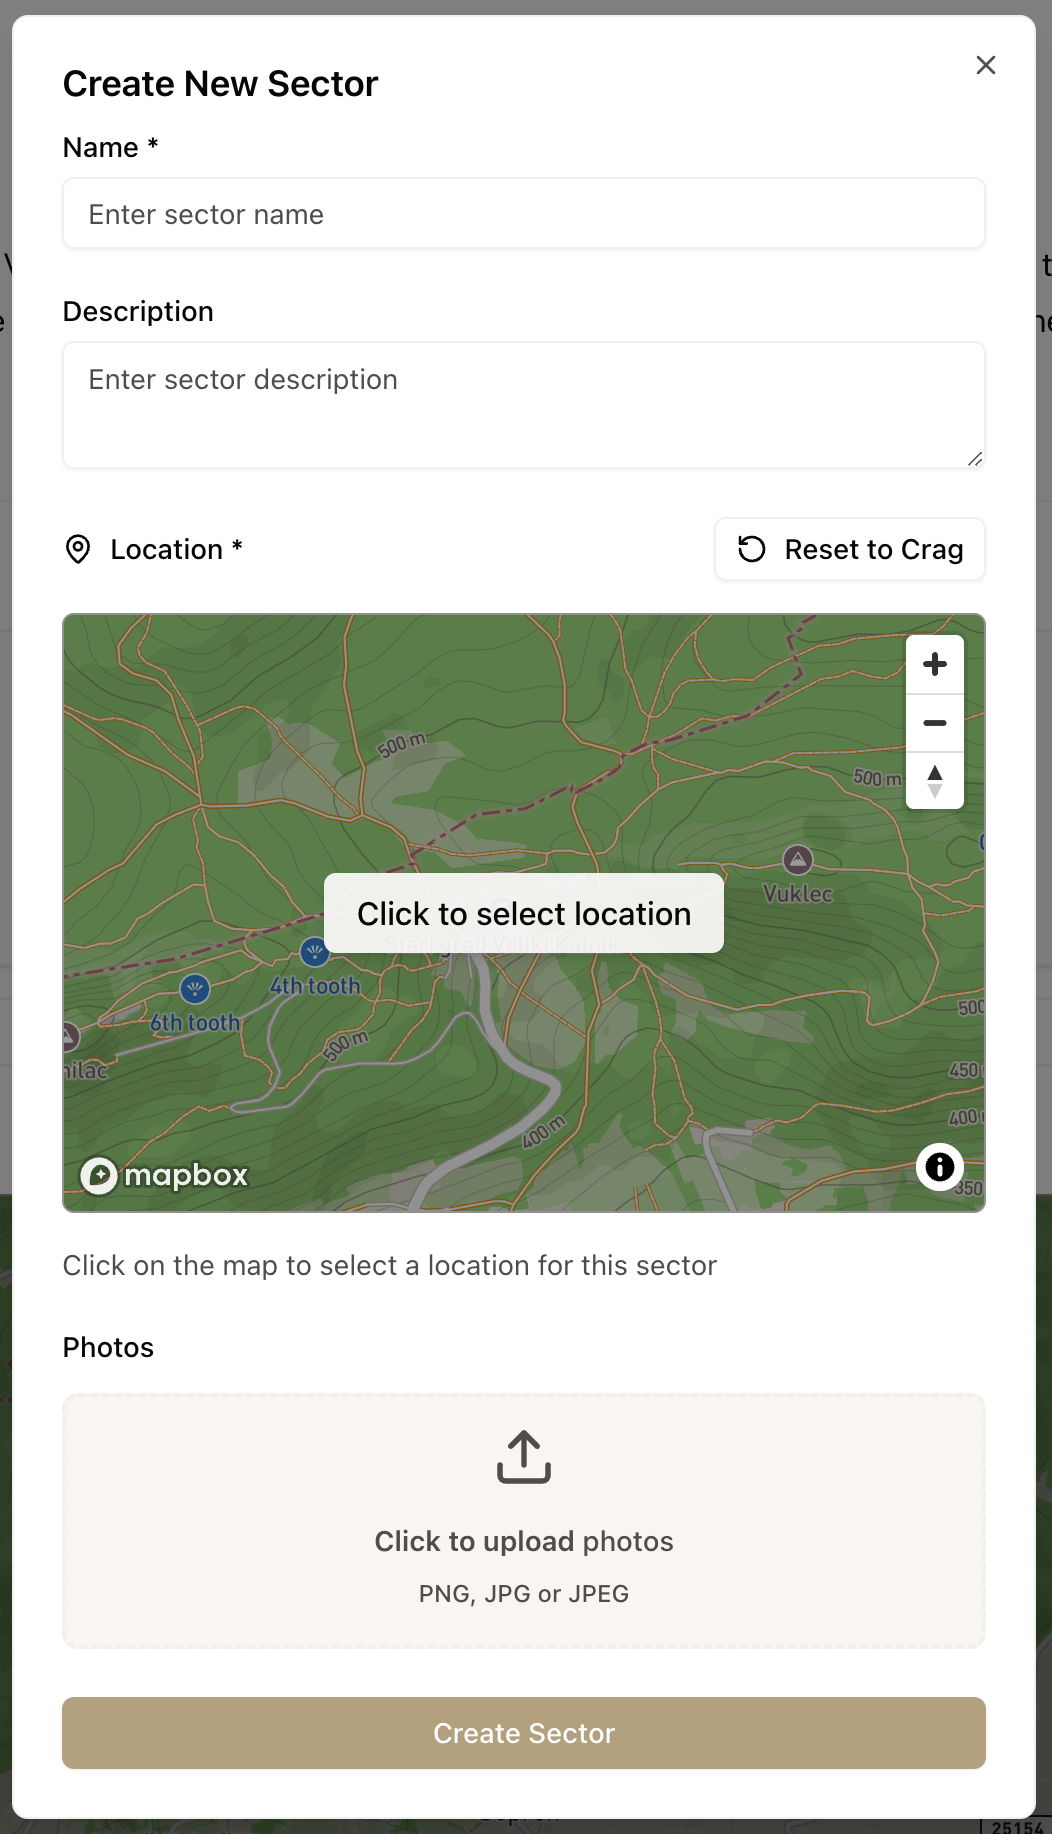
\includegraphics[width=\textwidth]{images/implementacija/web/editing-options/create-sector.png}
        \caption{Web aplikacija}
        \label{fig:dodavanje_sektora_web}
    \end{subfigure}
    \caption{Dodavanje novog sektora}
    \label{fig:dodavanje_sektora}
\end{figure}

Forma za unos novog sektora zahtijeva od korisnika unos naziva sektora i opcionalnog opisa, koji može sadržavati specifične informacije koje su specifične za sektore te ostale relevantne informacije (slika~\ref{fig:dodavanje_sektora}). Osim naziva zahtjeva se i upis lokacije u obliku koordinata. Pregledi taj proces olakšavaju uporabom geografske karte, koja omogućuje korisniku da odabere lokaciju sektora na karti ili pretraživanjem po nazivu lokacije. Kao i kod penjališta, moguće je dodati jednu ili više fotografija koje vizualno predstavljaju sektor.

Postojeći sektori mogu se uređivati na sličan način. Odabirom određenog sektora, korisniku se prikaže izbornik u kojem se nalazi opcija za uređivanje sektora. Forma omogućuje uređivanje  naziva, opisa, lokaciju i galeriju fotografija. (slika~\ref{fig:uredjivanje_sektora})

\begin{figure}[H]
    \centering
    \begin{subfigure}[b]{0.38\textwidth}
        \centering
        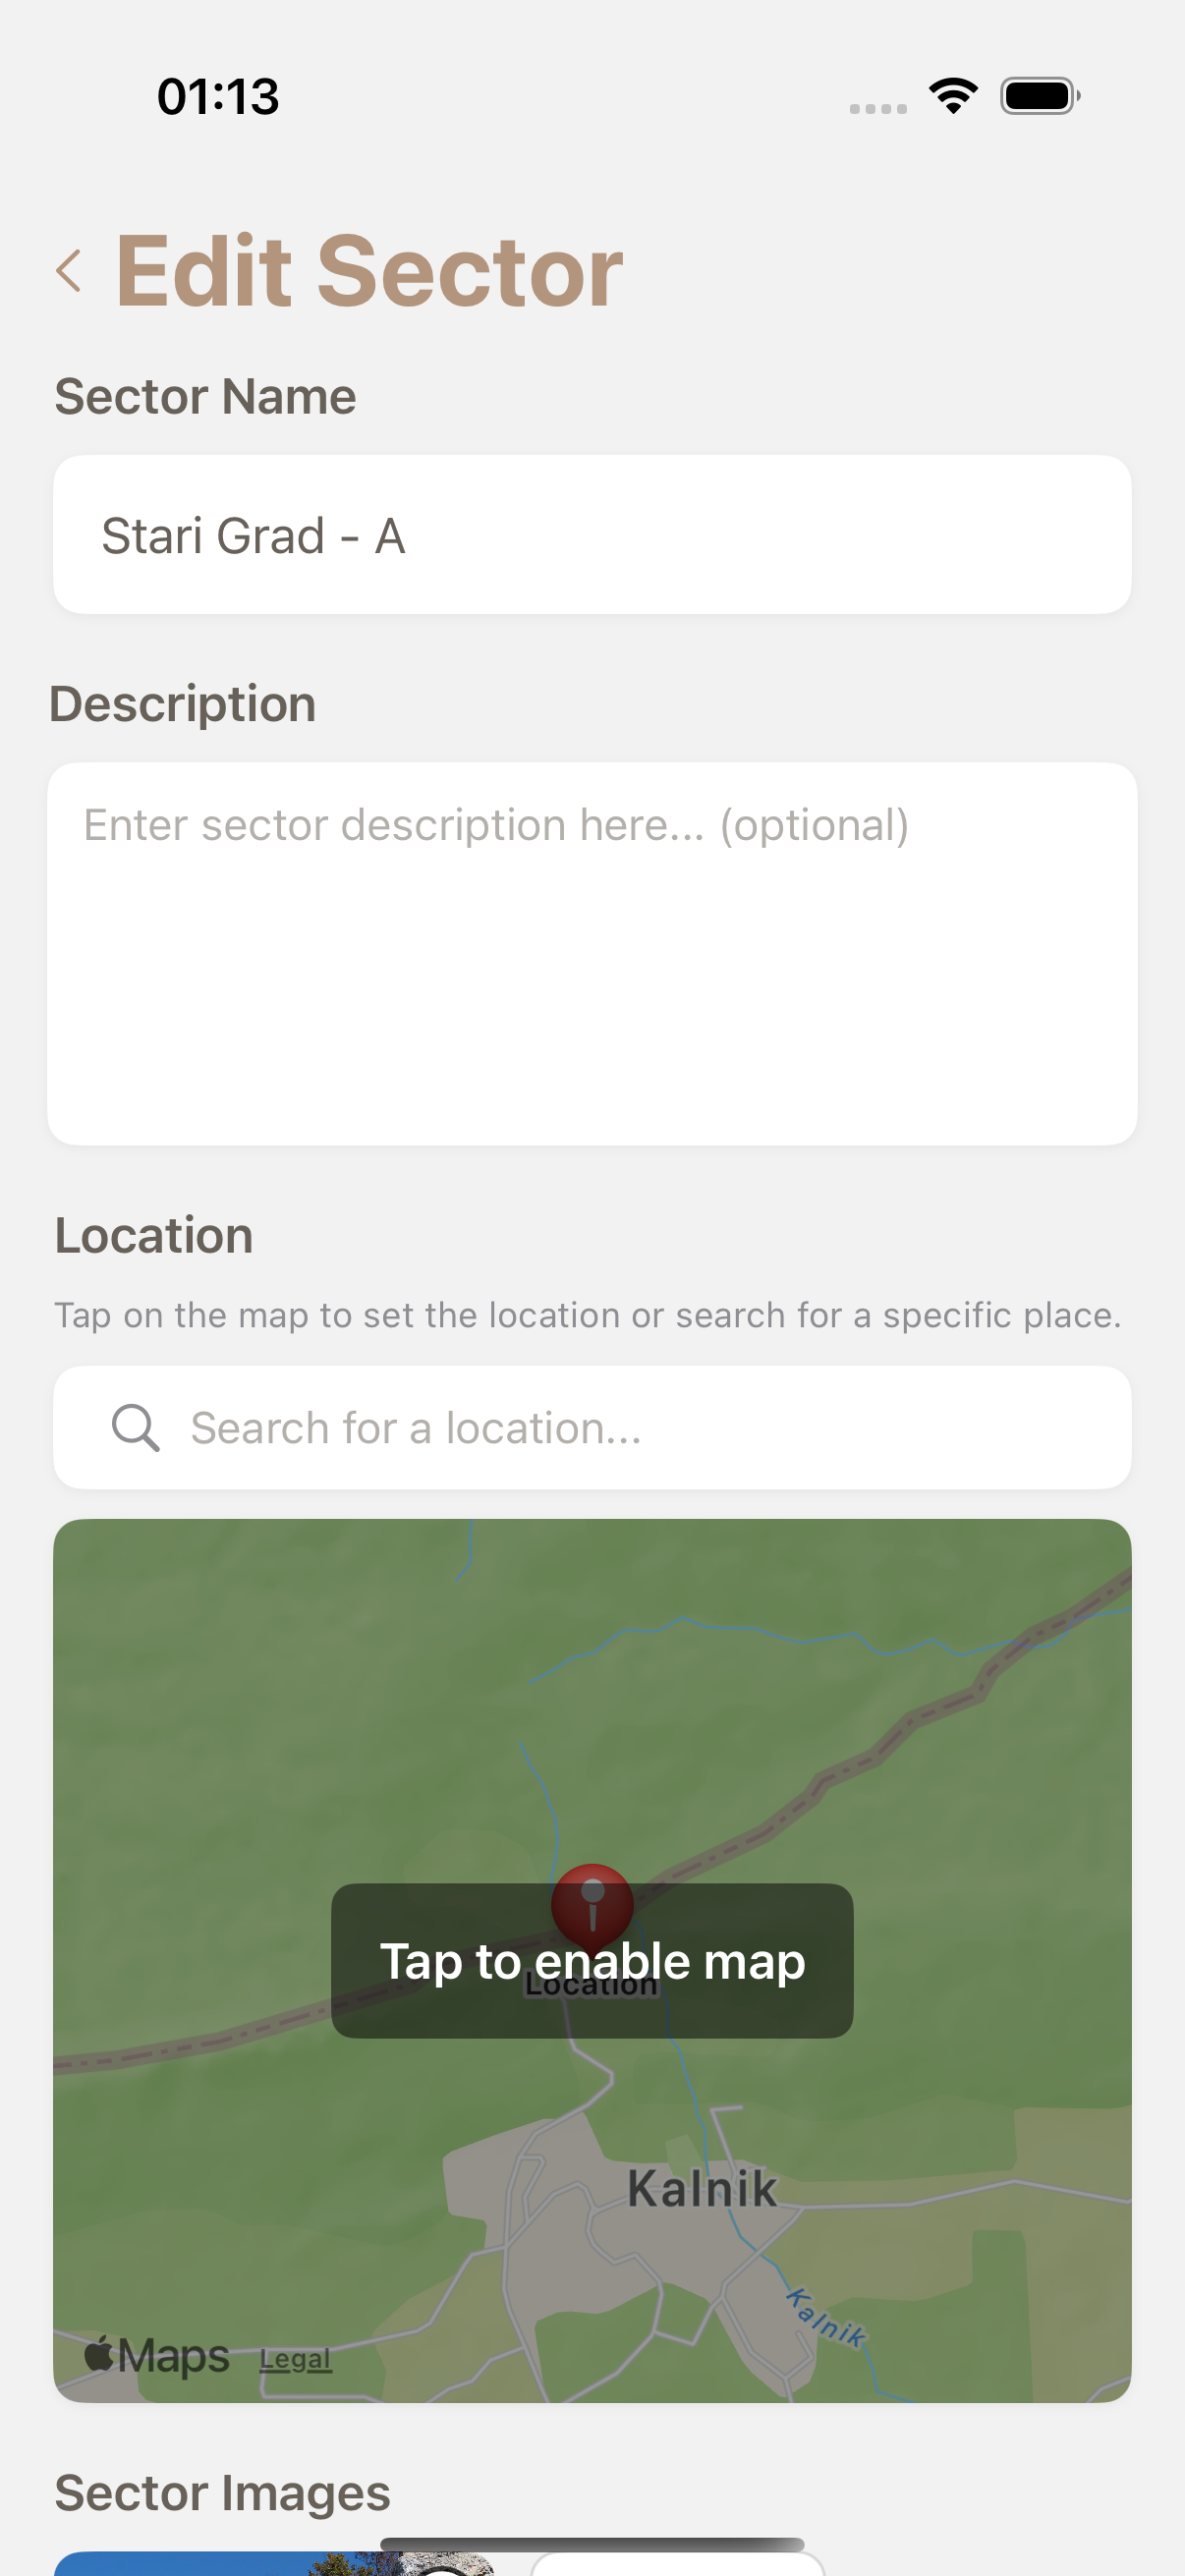
\includegraphics[width=\textwidth]{images/implementacija/editing-options/edit-sector.png}
        \caption{Mobilna aplikacija}
        \label{fig:uredjivanje_sektora_mob}
    \end{subfigure}
    \hfill
    \begin{subfigure}[b]{0.43\textwidth}
        \centering
        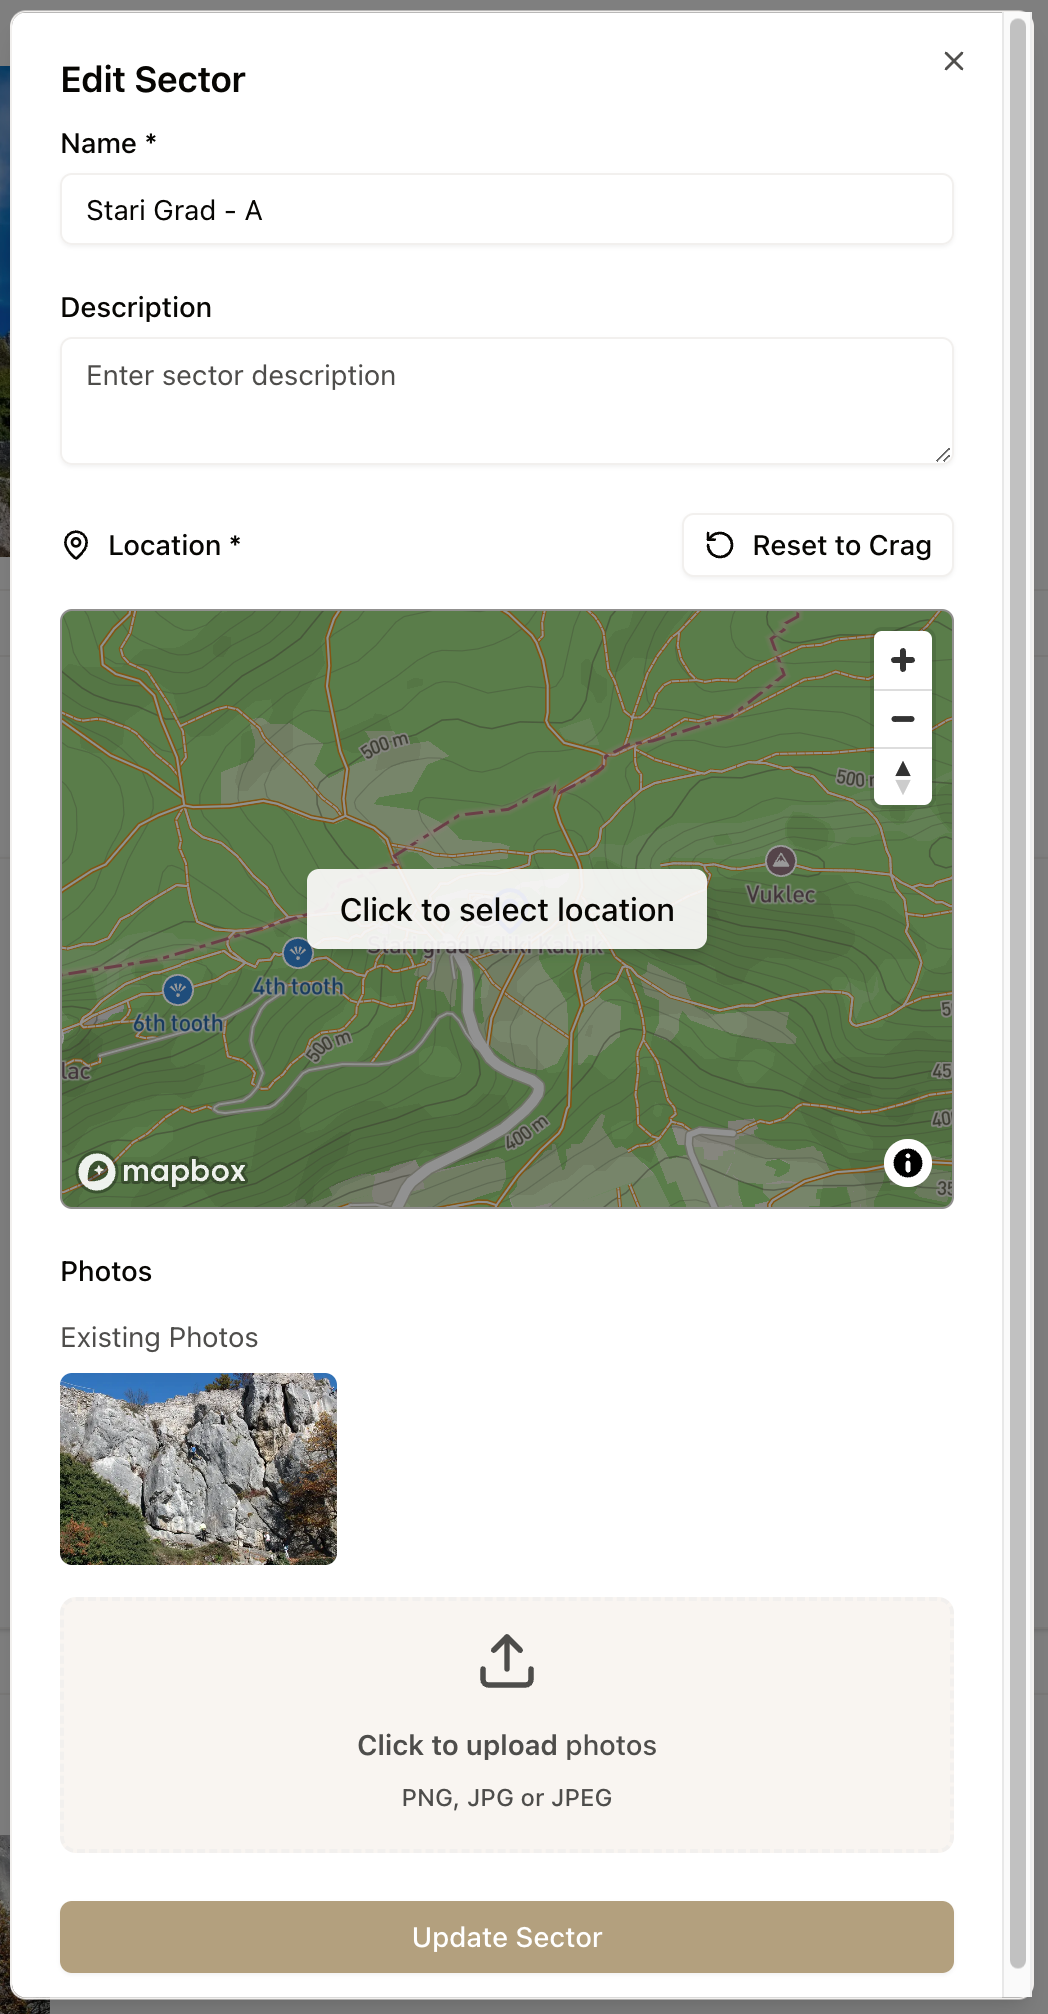
\includegraphics[width=\textwidth]{images/implementacija/web/editing-options/edit-sector.png}
        \caption{Web aplikacija}
        \label{fig:uredjivanje_sektora_web}
    \end{subfigure}
    \caption{Uređivanje postojećeg sektora}
    \label{fig:uredjivanje_sektora}
\end{figure}

Brisanje sektora dostupno je izborniku na zaslonu s detaljnim pregledom penjališta kada je označen penjački smjer. Klikom na opciju "Izbriši sektor" (eng. \textit{Delete sector}) korisniku se prikazuje prozor s upitom o potvrdi brisanja. Ako korisnik potvrdi brisanje, sektor se briše iz sustava i postaje nedostupno svim korisnicima.


\subsection{Dodavanje, uređivanje i brisanje penjačkih smjerova}

Na najnižoj hijerarhijskoj razini nalazi se unos i uređivanje pojedinačnih penjačkih smjerova. Ovlašteni korisnici mogu dodavati nove penjačke smjerove unutar određenog sektora. Pristup ovoj funkcionalnosti omogućen je u izborniku na zaslonu s detaljnim pregledom penjališta sa označenim sektorom. 

\begin{figure}[H]
    \centering
    \begin{subfigure}[b]{0.38\textwidth}
        \centering
        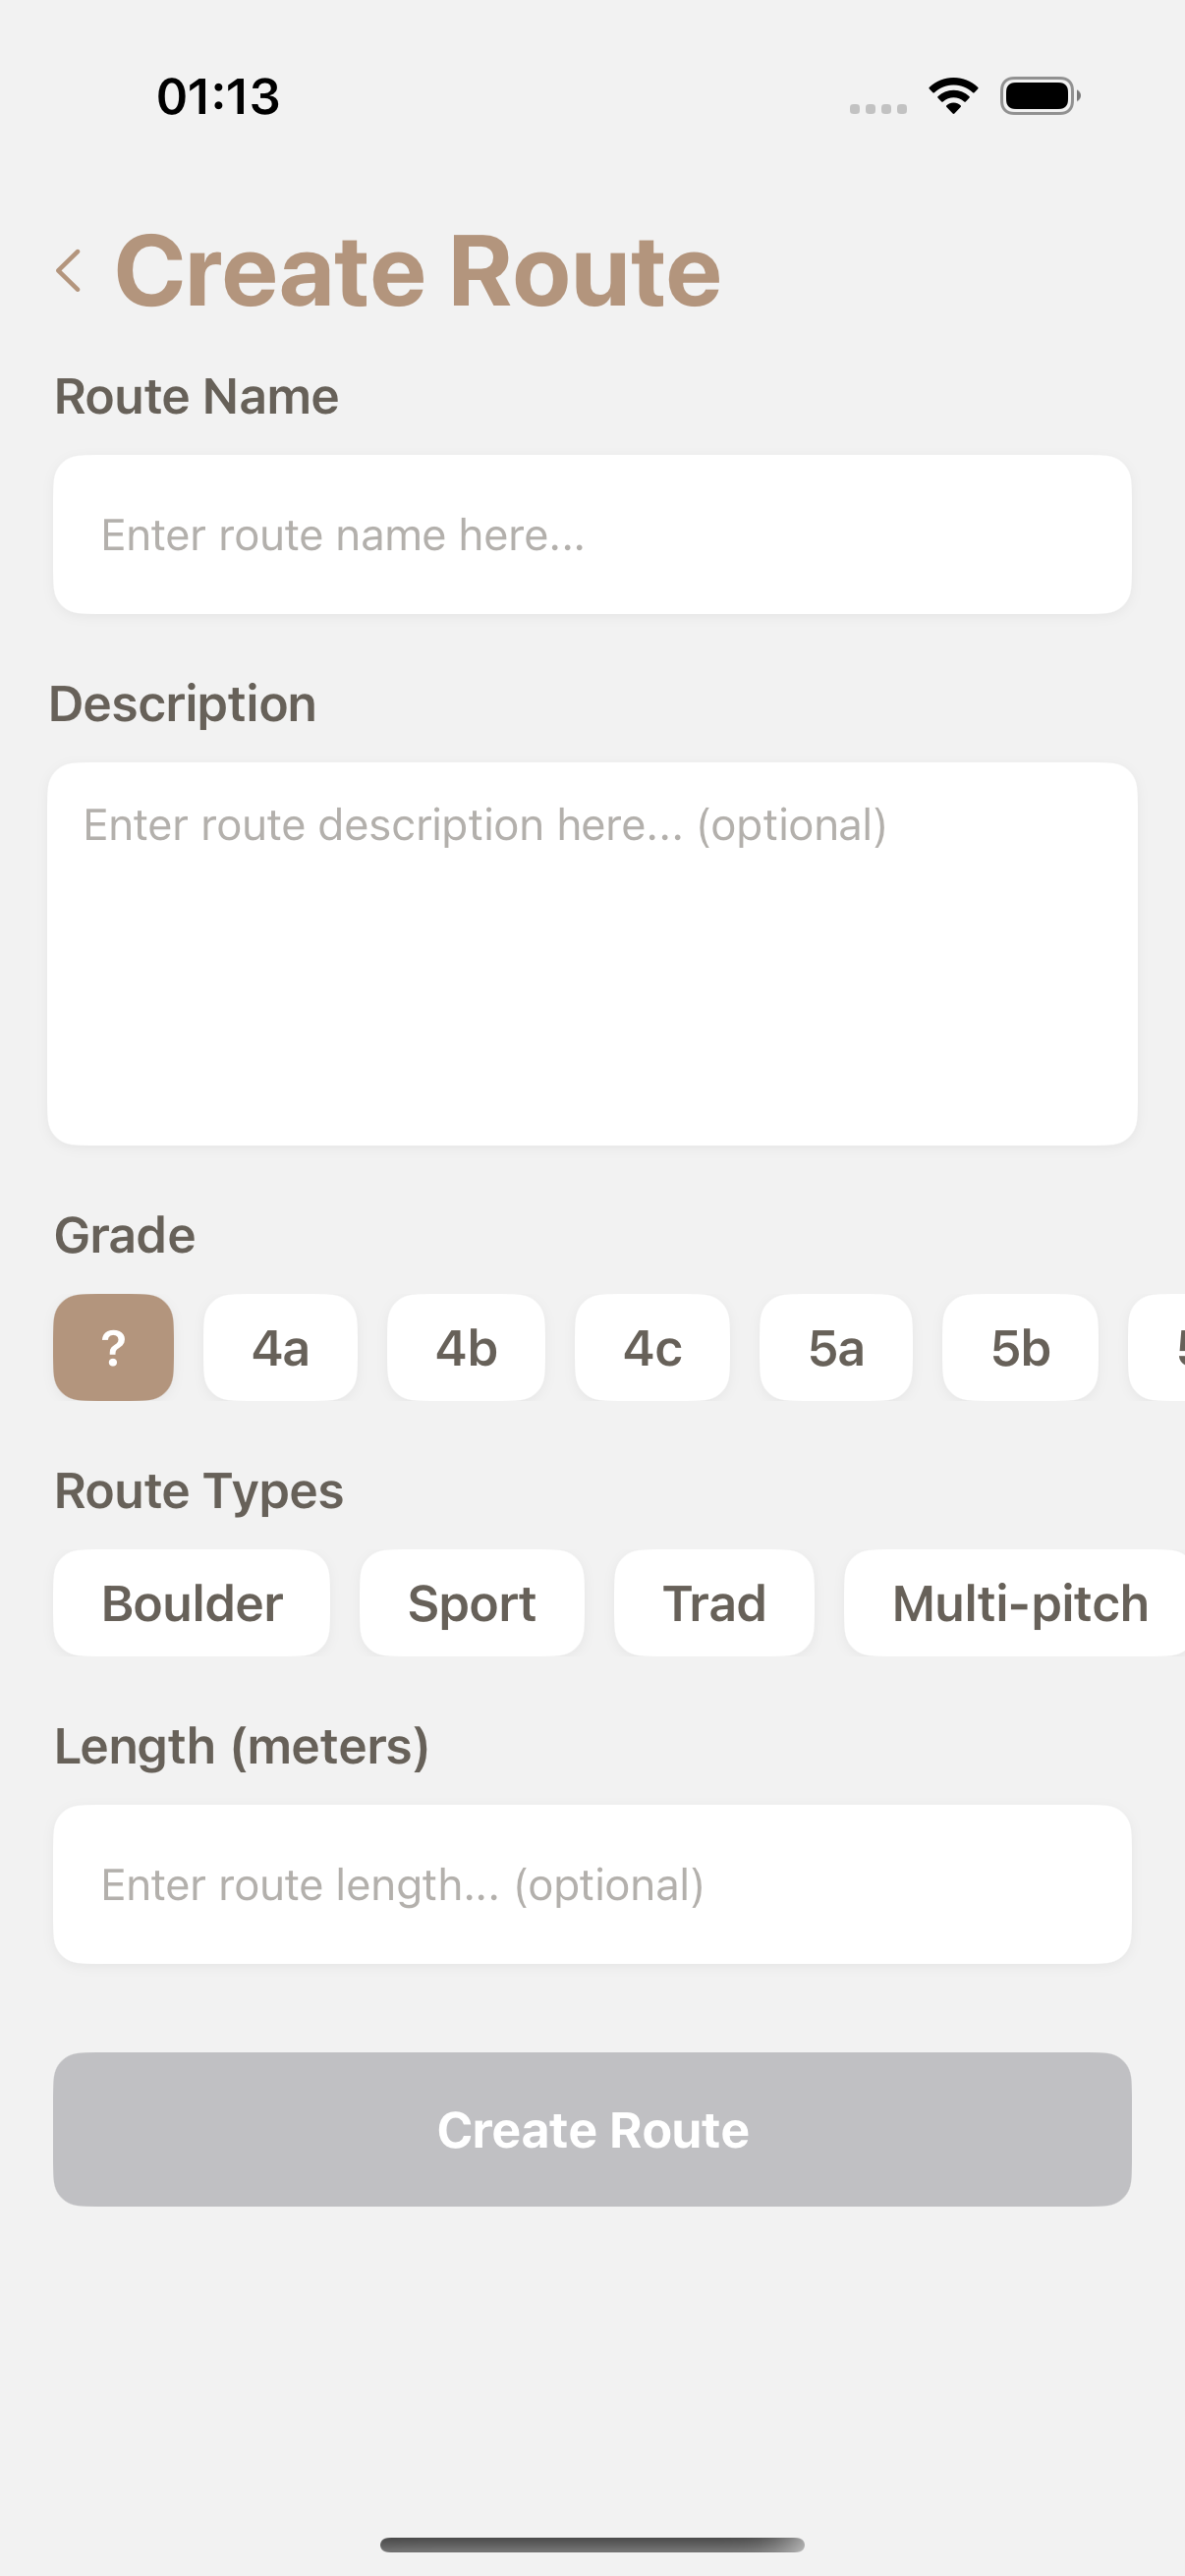
\includegraphics[width=\textwidth]{images/implementacija/editing-options/create-route.png}
        \caption{Mobilna aplikacija}
        \label{fig:dodavanje_smjera_mob}
    \end{subfigure}
    \hfill
    \begin{subfigure}[b]{0.55\textwidth}
        \centering
        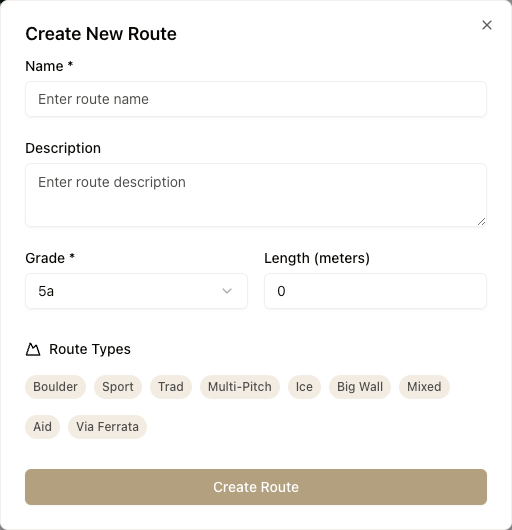
\includegraphics[width=\textwidth]{images/implementacija/web/editing-options/create-route.png}
        \caption{Web aplikacija}
        \label{fig:dodavanje_smjera_web}
    \end{subfigure}
    \caption{Dodavanje novog penjačkog smjera}
    \label{fig:dodavanje_smjera}
\end{figure}

Forma za kreiranje novog penjačkog smjera uključuje polja poput naziva, opisa, težine, tipa penjačkog smjera i dužine (slika~\ref{fig:dodavanje_smjera}). Opcije za tip penjačkog smjera uključuju boulder, sportski, tradicionalni ili smjer s više penjačkih smjerova. 
Važno je primjetiti kako opcija dodavanja slike penjačkog smjera nije dostupna u formi za dodavanje novog penjačkog smjera. Dodavanje fotografije je moguće nakon kreiranja penjačkog smjera u pregledu detalja penjačkog smjera i dostupno je samo na mobilnoj aplikaciji. Klikom na izbornik u gornjem desnom kutu pregleda detalja penjačkog smjera, korisniku se prikazuje izbornik u kojem se nalazi opcija za dodavanje fotografije. Prvi korak u procesu dodavanja fotografije je slikanje penjačkog smjera pomoću kamere mobilnog uređaja. Nakon slikanja, korisniku se prikazuje slika na koju se može ručno ucrtati linija penjačkog smjera. Time je korisnik kreirao referentnu sliku penjačkog smjera koja se može koristiti za prepoznavanje penjačkog smjera (slika~\ref{fig:dodavanje_fotografije_smjera}).

\begin{figure}[H]
    \centering
    \includegraphics[width=0.3\textwidth]{images/implementacija/editing-options/add-route-photo.png}
    \caption{Dodavanje fotografije penjačkog smjera}
    \label{fig:dodavanje_fotografije_smjera}
\end{figure}

Uređivanje postojećeg penjačkog smjera dostupno je u izborniku na zaslonu s detaljnim pregledom tog penjačkog smjera. Na web aplikaciji izbornik se nalazi na izborniku u tablici kada je označen pregled svih sektora ili u listi kada je označen neki sektor. 

\begin{figure}[H]
    \centering
    \begin{subfigure}[b]{0.38\textwidth}
        \centering
        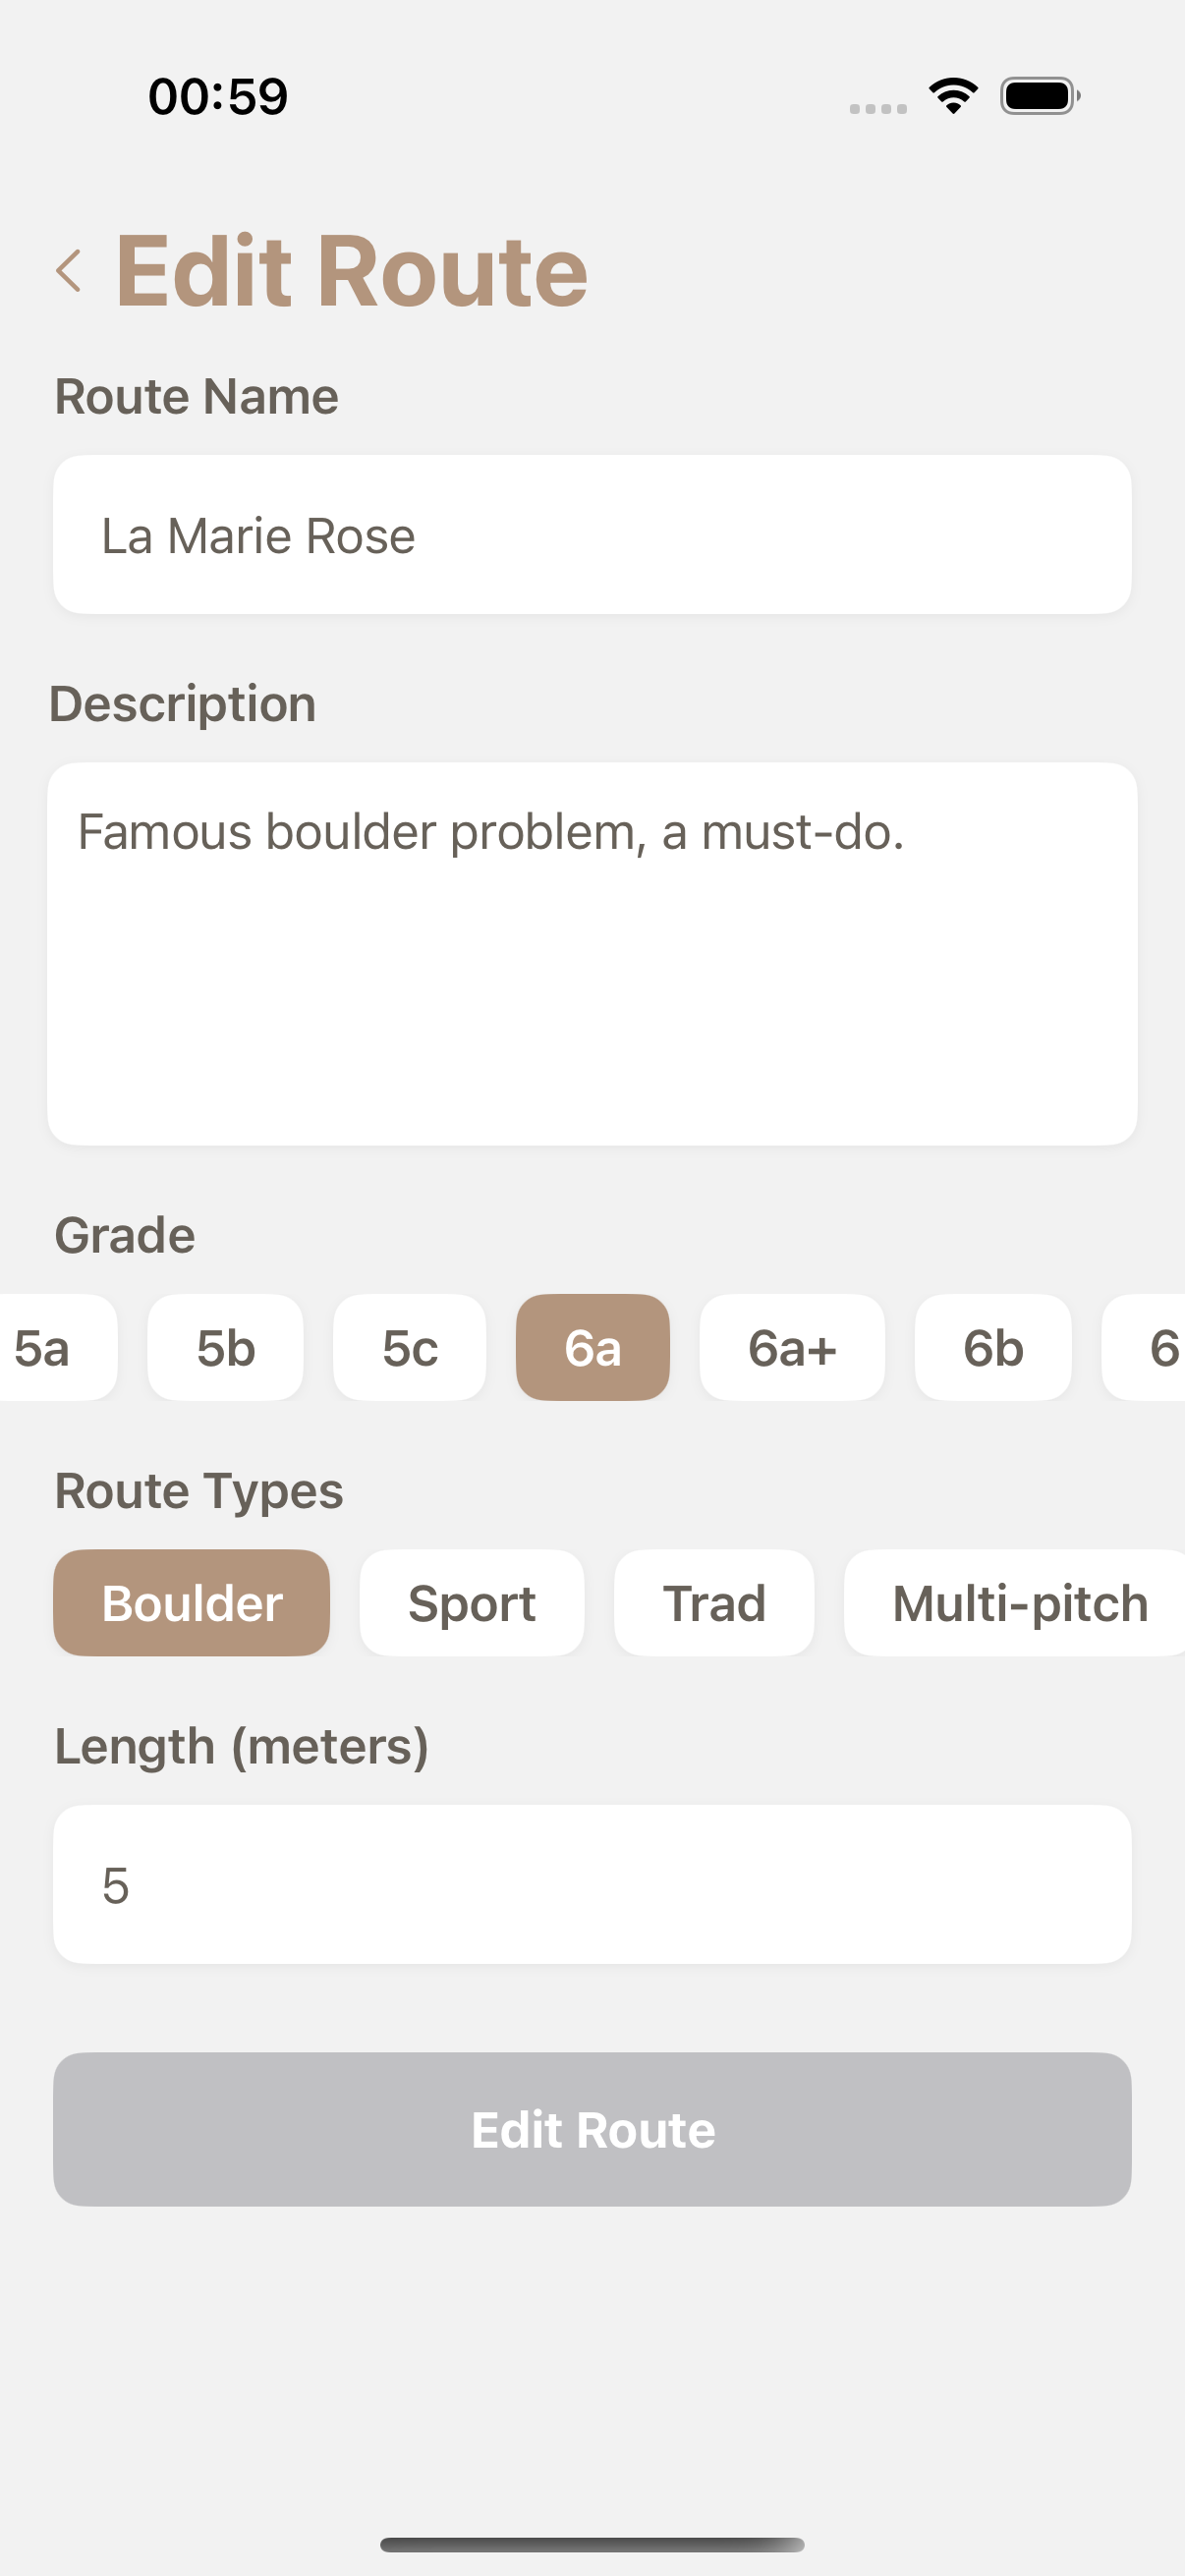
\includegraphics[width=\textwidth]{images/implementacija/editing-options/edit-route.png}
        \caption{Mobilna aplikacija}
        \label{fig:uredjivanje_smjera_mob}
    \end{subfigure}
    \hfill
    \begin{subfigure}[b]{0.55\textwidth}
        \centering
        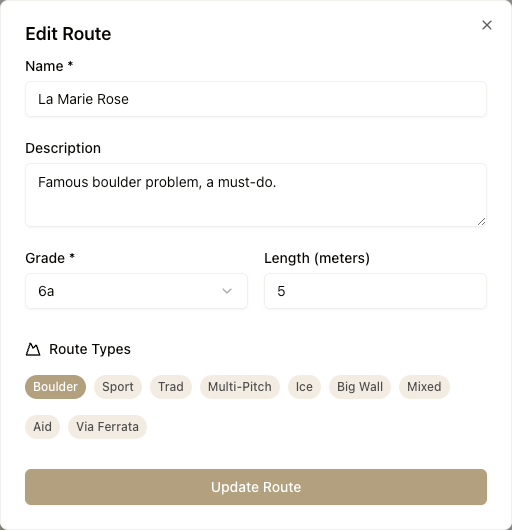
\includegraphics[width=\textwidth]{images/implementacija/web/editing-options/edit-route.png}
        \caption{Web aplikacija}
        \label{fig:uredjivanje_smjera_web}
    \end{subfigure}
    \caption{Uređivanje postojećeg penjačkog smjera}
    \label{fig:uredjivanje_smjera}
\end{figure}

Forma omogućuje uređivanje svih podataka o penjačkom smjeru, uključujući naziv, opis, težinu, tip penjačkog smjera i dužinu, no također je omogućuje brisanje fotografija penjačkog smjera (slika~\ref{fig:uredjivanje_smjera}).


Brisanje penjačkog smjera dostupno je u izborniku na zaslonu s detaljnim pregledom penjačkog smjera. Klikom na opciju "Izbriši smjer" (eng. \textit{Delete route}) korisniku se prikazuje prozor s upitom o potvrdi brisanja. Ako korisnik potvrdi brisanje, penjački smjer se briše iz sustava i postaje nedostupno svim korisnicima.


\subsection{Uređivanje korisničkog profila}

Unutar korisničkog profila, u gornjem desnom kutu, nalazi se izbornik koji sadrži dodatne opcije za upravljanje računom i, ovisno o korisnikovim ovlastima, za doprinos sadržaju aplikacije. Odabirom opcije "Uredi profil" (eng. \textit{Edit profile}) korisnik odlazi na stranicu za uređivanje svojih podataka. Moguće je promijeniti ime, prezime, korisničko ime i datum rođenja. Aplikacija također omogućuje promjenu profilne fotografije te ažuriranje lozinke (slika~\ref{fig:uredjivanje_profila}).

\begin{figure}[H]
    \centering
    \begin{subfigure}[b]{0.35\textwidth}
        \centering
        \includegraphics[width=\textwidth]{images/implementacija/editing-options/edit_profile.png}
        \caption{Mobilna aplikacija}
        \label{fig:uredjivanje_profila_mob}
    \end{subfigure}
    \hfill
    \begin{subfigure}[b]{0.55\textwidth}
        \centering
        \includegraphics[width=\textwidth]{images/implementacija/web/editing-options/edit-user.png}
        \caption{Web aplikacija}
        \label{fig:uredjivanje_profila_web}
    \end{subfigure}
    \caption{Uređivanje korisničkog profila}
    \label{fig:uredjivanje_profila}
\end{figure}
\section{Izvanmrežni način rada}

Penjališta se često nalaze na udaljenim lokacijama s ograničenim ili nepostojećim internetskim signalom. Zbog toga aplikacija implementira izvanmrežni način rada kako bi omogućila korisnicima korištenje aplikacije i situacijama slabog internetskog signala. Ova mogućnost je dostupna samo na mobilnoj aplikaciji. Korisnik može preuzeti podatke za bilo koje penjalište ili penjački smjer unutar detaljnog pregleda penjališta ili penjačkog smjera klikom na "Preuzmi penjalište" (eng. \textit{Download crag}) ili "Preuzmi penjački smjer" (eng. \textit{Download route}). Aplikacija tada pohranjuje sve podatke na lokalni uređaj, uključujući informacije o sektorima i penjačkim smjerovima, galerije forografija te najvažnije, referentne slike penjačkh smjerova potrebne za rad funkcionalnosti prepoznavanja penjačkih smjerova.

\begin{figure}[H]
    \centering
    \begin{subfigure}[b]{0.4\textwidth}
        \centering
        \includegraphics[width=0.7\textwidth]{images/implementacija/offline-mode/crag-tab.png}
        \caption{Popis preuzetih penjališta}
        \label{fig:offline_crag_tab}
    \end{subfigure}
    \hspace{0.08\textwidth}
    \begin{subfigure}[b]{0.4\textwidth}
        \centering
        \includegraphics[width=0.7\textwidth]{images/implementacija/offline-mode/routes-tab.png}
        \caption{Popis preuzetih penjačkih smjerova}
        \label{fig:offline_routes_tab}
    \end{subfigure}
    \caption{Izvanmrežni način rada - pregled preuzetih penjališta i smjerova}
    \label{fig:izvanmrezni_nacin_rada}
\end{figure}

Pristupom izvanmrežnom načinu rada, korisniku se prikazuje sučelje (slika~\ref{fig:izvanmrezni_nacin_rada}) s popisom svih penjališta i pojedinačnih penjačkih smjerova koje je prethodno preuzeo. Unutar ovog načina, korisnik može pregledavati sve preuzete podatke na gotovo identičan način kao i kada je spojen na internet. Detaljni pregled penjališta i smjerova zadržava sve ključne informacije i komponente, s iznimkom onih koje ovise o vanjskim servisima, poput vremenske prognoze i uređivanje podataka.
Najvažnije, funkcionalnost prepoznavanja penjačkih smjerova pomoću proširene stvarnosti je dostupna u izvanmrežnom načinu rada. Budući da su sve referentne slike pohranjene lokalno, proces detekcije i vizualizacije može se izvršavati neovisno o internetskoj vezi. Time se osigurava da ta funkcionalnost je dostupna penjačima upravo gdje je najpotrebnija - ispred same stijene.

